\documentclass[12pt,a4paper]{article}

% --- Preamble ---
\usepackage[utf8]{inputenc} % Allows UTF-8 input
\usepackage[T1]{fontenc}    % Recommended font encoding
\usepackage[english]{babel} % Language settings

% Maths and symbols
\usepackage{amsmath}
\usepackage{amssymb}
\usepackage{amsfonts}

\usepackage{tikz}
\usetikzlibrary{shapes.geometric, arrows, positioning, fit, backgrounds}

% Graphics
\usepackage{graphicx} 
\graphicspath{{./images/}} 

% Tables
\usepackage{booktabs} 
\usepackage{multirow} 

% Commenting
\usepackage{comment}

% Math and QC
\usepackage{mathtools}
\DeclarePairedDelimiter\bra{\langle}{\rvert}
\DeclarePairedDelimiter\ket{\lvert}{\rangle}
\DeclarePairedDelimiterX\braket[2]{\langle}{\rangle}{#1\,\delimsize\vert\,\mathopen{}#2}

% Multicols
\usepackage{multicol}

\usepackage{quantikz}

% Subfigures
\usepackage{subcaption}

% Float for [H] placement
\usepackage{float}

% Code highlighting configuration
\usepackage{listings}
\definecolor{codegreen}{rgb}{0,0.6,0}
\definecolor{codegray}{rgb}{0.5,0.5,0.5}
\definecolor{codepurple}{rgb}{0.58,0,0.82}
\definecolor{backcolour}{rgb}{0.96,0.96,0.94}

\lstset{
	backgroundcolor=\color{backcolour},
	commentstyle=\color{codegreen},
	keywordstyle=\color{magenta},
	numberstyle=\tiny\color{codegray},
	stringstyle=\color{codepurple},
	basicstyle=\ttfamily\footnotesize,
	breaklines=true,
	captionpos=b,
	keepspaces=true,
	numbers=left,
	showspaces=false,
	showstringspaces=false,
	language=Python
}

% Bibliography
\usepackage{cite} 

% Hyperlinks
\usepackage{hyperref} 
\hypersetup{
	colorlinks=true,
	linkcolor=blue,
	filecolor=magenta,
	urlcolor=cyan,
}

% Customization
\usepackage{geometry} 
\geometry{
	a4paper,
	top=2.5cm,
	bottom=2.5cm,
	left=3cm,
	right=2.5cm,
	heightrounded,
	footskip=1cm,
}

% Color and highlighting for tracking changes
\usepackage{xcolor}
\usepackage{soul}
\usepackage[normalem]{ulem}

% Revision commands
\newcommand{\add}[1]{\textcolor{green!50!black}{#1}}
\newcommand{\del}[1]{\textcolor{red}{\sout{#1}}}
\newcommand{\rephrase}[1]{\textcolor{orange}{#1}}

% Title page details
\title{Upgrade Progress Report}
\author{Faiez Altamimi
	\\ \textit{Supervised by Prof. Mohammad Mousavi}
	\\ \textit{\& Supervised by Dr. Gunel Jahangirova}
}

\date{Feb 2026}

% Appendices
\usepackage[toc,page]{appendix} 

% --- Main Document ---
\begin{document}
	
	\maketitle 
	
	\begin{abstract}
		This report provides a summary of the research progress achieved during the PhD study of Faiez Altamimi from October 1st, 2024 to Feb 10th, 2026. It outlines the research, what has been completed, key findings, challenges encountered, and plans for the next reporting period.
	\end{abstract}
	
	\tableofcontents 
	\newpage 
	
	\section{Introduction}
	\label{sec:introduction}
	
	Quantum Computing (QC) harnesses its distinctive properties—such as superposition and entanglement—to solve numerous complex problems. Yet, QC applications remain uncommon, mainly due to the challenges in its software development. Many classical software developers lack the required knowledge to develop quantum circuits. To bridge this gap, many software engineering techniques, tools and methods are being adapted to QC to facilitate the development experience. One of the mandatory areas of software engineering, essential for robust QC development, is software testing.
	
	The primary challenge in quantum software testing is the oracle problem, i.e., the lack of software specification \cite{9036058}. The other challenges in QC software testing are: scarcity of QC programs, QC probabilistic nature, destructive measurement \cite{wang2023qucatcombinatorialtestingtool} and that QC development involves the usage of low-level circuits and gates. In order to address the difficulties in testing QC programs \cite{garousi2020software}, different classical testing techniques were adopted for QC e.g., mutation testing \cite{9844849}, fuzz testing \cite{wang2018quanfuzzfuzztestingquantum}, metamorphic testing \cite{10.1145/3528230.352918}, and differential testing. One of the prominent testing techniques is metamorphic testing (MT). It is a property-based testing method, which treats the system under test (SUT) as a black box. 
	
	Moreover, QC is considered a good fit for Artificial Intelligence (AI) and specifically for machine learning (ML) algorithms, which indicates that the field of quantum machine learning (QML) is a promising field. Similarly to QC, ML programs also can be treated as black boxes in software testing, and therefore QML algorithms are particularly suitable to be tested as black boxes. The goal of Quantum Machine Learning is not only to accelerate algorithms i.e., make them faster, but also to leverage the fundamental principles of quantum mechanics to develop novel processing methods. We will be exploring most of the notable QML algorithms during the next couple of years e.g., Quantum Neural Networks (QNNs) and Quantum Convolutional Neural Networks (QCNNs) algorithms.
	
	In general, one of the most common ML algorithms for QC is support vector machines (SVM). There are different types of machine learning algorithms e.g., supervised learning, unsupervised learning and reinforcement learning. SVM is a supervised learning algorithm that is used for data classification and regression. SVM implements a kernel that calculates the data similarity using an inner product while avoiding the intensive computation, without ever explicitly mapping the data into that space. This allows the algorithm to find complex patterns by operating as if it were working in a higher dimension, but with the computational cost of the original dimension. One of the ways to utilize QC with SVM is to implement a quantum counterpart of the kernel with SVM, which is known as QSVM. The quantum kernel will expedite the learning process in QSVM compared to the classical SVM \cite{Rebentrost_2014} \cite{Gentinetta_2024}. In this work, we will use metamorphic testing (MT) to test QSVM as a black box system along with mutation analysis and statistical testing. 
	
	Section \ref{sec:preliminaries} goes through the preliminaries about QC and software testing.  Section \ref{sec:LiteratureReview} will review the literature and relatively recent research around software testing with quantum programs and machine learning algorithms. Section \ref{sec:LiteratureReview} will go through the literature review. Section \ref{sec:evaluation} elaborates the challenges faced, the subsequent solutions, and the advanced experimentation. Section 4 explains the metamorphic relations for the QSVM. Section 5 evaluates the effectiveness of these metamorphic relations, provides the results, and discuss them. Section \ref{sec:conclusion} Draws a conclusion to this work and shows the work plan for the next period.
	
	
	\section {Preliminaries}
	\label{sec:preliminaries}
	
	\subsection{Quantum Computing}
	
	Quantum Computers use qubits to represent information and apply quantum gates  on the qubits to transform their states. Below, the states for $0$ and $1$ are represented using kets, where a ket is a vector:
	
	\begin{multicols}{2}
		\begin{equation*}
			\ket{0} = \begin{bmatrix}
				1 \\ 0
			\end{bmatrix}\\
		\end{equation*}
		
		\begin{equation*}
			\ket{1} = \begin{bmatrix}
				0 \\ 1
			\end{bmatrix}
		\end{equation*}
	\end{multicols}
	
	In Quantum Computing qubits can be in a superposition state until measured. Superposition is a property that indicates that the qubit is in a linear combination of different states at once. The general formula of a superposition is as follows:
	
	\begin{align*}
		\ket{\Psi} &= \alpha\ket{0} + \beta\ket{1} 
	\end{align*}
	
	where $\alpha$ and $\beta$ are probability amplitudes that should satisfy the following constraint:
	
	\begin{align*}
		|\alpha|^2 + |\beta|^2 &= 1
	\end{align*}
	
	To visualize the state of any single qubit, the Bloch sphere is used, and it shows the state in a three dimensional space. There are multiple quantum gates for one or more qubits. One of the quantum gates is the CNOT gate, which takes two qubits as inputs and gives two qubits as outputs, which is shown in Figure \ref{fig:1} and Table \ref{table:1} is the truth table for the CNOT gate.
	
	\begin{figure}[H]
		\centering
		\begin{quantikz}[row sep={9mm,between origins}]
			\lstick{$\ket{X}$} & \ctrl{1} & \ket{X} \\
			\lstick{$\ket{Y}$} & \targ{} & \ket{X} \oplus \ket{Y}
		\end{quantikz}
		\caption{Quantum CNOT gate}
		\label{fig:1}
	\end{figure}
	
	\begin{table}[H]
		\centering
		\begin{tabular}{|c c c c|} 
			\hline
			\multicolumn{4}{|c|}{CNOT gate} \\ [0.5ex]
			\hline
			\multicolumn{2}{|c|}{Input} & \multicolumn{2}{c|}{output} \\ [0.5ex] 
			\hline
			\multicolumn{1}{|c|}{X} & \multicolumn{1}{|c|}{Y} & \multicolumn{1}{|c|}{X} & \multicolumn{1}{|c|}{X $\oplus$ Y} \\ [0.5ex] 
			\hline
			\multicolumn{1}{|c}{ $\ket{0}$} & \multicolumn{1}{|c|}{ $\ket{0}$} & \multicolumn{1}{|c|}{ $\ket{0}$} & \multicolumn{1}{c|}{ $\ket{0}$} \\ 
			\hline
			\multicolumn{1}{|c}{ $\ket{0}$} & \multicolumn{1}{|c|}{ $\ket{1}$} & \multicolumn{1}{|c|}{ $\ket{0}$} & \multicolumn{1}{c|}{$\ket{1}$} \\ 
			\hline
			\multicolumn{1}{|c}{$\ket{1}$} & \multicolumn{1}{|c|}{ $\ket{0}$} & \multicolumn{1}{|c|}{$\ket{1}$} & \multicolumn{1}{c|}{$\ket{1}$} \\ 
			\hline
			\multicolumn{1}{|c}{$\ket{1}$} & \multicolumn{1}{|c|}{$\ket{1}$} & \multicolumn{1}{|c|}{$\ket{1}$} & \multicolumn{1}{c|}{ $\ket{0}$} \\ 
			\hline
		\end{tabular}
		\caption{CNOT Gate Truth Table}
		\label{table:1}
	\end{table}
	
	From the truth table above, the value of the target qubit $Y$ is inverted or not based on the value of the control qubit $X$. For example, if we have $X \otimes Y =$ $ (\frac{1}{\sqrt2}\ket{0} + \frac{1}{\sqrt2}\ket{1}) \otimes \ket{1} =  \frac{1}{\sqrt2}\ket{01} + \frac{1}{\sqrt2}\ket{11}$.  The part of $\frac{1}{\sqrt2}\ket{11}$ will change to $\frac{1}{\sqrt2}\ket{10}$ since the control qubit (first qubit) is $1$ which will change the other qubit from $1$ to $0$. Then the result of the CNOT gate according to the CNOT gate truth table \ref{table:1} will be $ \frac{1}{\sqrt2}\ket{01} + \frac{1}{\sqrt2}\ket{10}$. The result is known as one of the Bell states, and these states are two qubits states that are maximally entangled.
	
	Another quantum gate is the Hadamard gate. It takes a state of $\ket{0}$ or $\ket{1}$ and turns that state into a superposition of $\ket{0}$ and $\ket{1}$, which is represented as a matrix as shown below:
	
	\begin{equation}
		\label{eqn:equation1}
		\frac{1}{\sqrt{2}} \begin{bmatrix*}
			1 & 1\\ 1 & -1
		\end{bmatrix*}\\
	\end{equation}
	
	Hadamard can be used to put any qubit in a superposition. If it takes $\ket{0}$, then the output will be 
	$\frac{1}{\sqrt{2}} (\ket{0} +\ket{1})$. And if the input is $\ket{1}$, then the output will be $\frac{1}{\sqrt{2}} (\ket{0} -\ket{1})$. And if combined with a CNOT gate, an entanglement between two qubits can be generated. Both superposition and entanglement phenomena are the reasons why quantum computers can execute algorithms much faster than classical computers \cite{9357505}.
	
	Other quantum gates are as follows:
	\begin{itemize}
		\item Pauli-X: is an inverter gate
		\item Pauli-Z: is a phase flipping gate around Z-axis
		\item Pauli-Y: is a gate that causes rotation around the Y-axis by $\pi$ radians
	\end{itemize}
	The five aforementioned gates can be used to approximately create any quantum circuit. 
	
	Furthermore, Quantum Fourier Transform (QFT) is one of the building blocks in quantum computers and many advanced algorithms are based on it, but it needs quantum computers that are immune to noise. QFT is represented for any basis state $J$ as:
	
	\begin{equation}
		\label{eqn:equation2}
		QFT\ket{j} =  \frac{1}{\sqrt{2}} \sum_{k=0}^{2^n-1} e^\frac{2\pi ijk}{2n} \ket{k}
	\end{equation}
	
	Quantum Phase Estimation (QPE) is based on QFT and it allows us to find the eigenvalue of an eigenvector for a given matrix. There are many other advanced quantum algorithms. However due to the limitations of NISQ devices, many algorithms are being developed as NISQ algorithms to be implemented in the near term e.g., Quantum Approximate Optimization Algorithm (QAOA), and Variational Quantum Eigensolver (VQE). 
	
	\subsection{Quantum Machine Learning (QML) \& Quantum Support Vector Machines (QSVM) }
	
	Some of the Machine Learning (ML) algorithms can utilize QC capabilities to enhance their efficiency, specifically on complex datasets \cite{electronics12112379} \cite{maouaki2024quantumsupportvectormachine}. Like any QC program/algorithm, QML algorithms can vary based on the implementation complexity. Some can be realized with a hybrid system using quantum along with classical computers and by using NISQ devices, and some others might need Fault-Tolerant quantum computers (FTQC). One of the promising QML algorithms is Quantum Support Vector Machines (QSVM), since it is using a kernel that instead of needing an intensive classical computational power, it can utilize a suitable quantum kernel. Next we will elaborate on how Support Vector Machine (SVM) works and accordingly how QSVM works.
	
	For a binary classification problem, we have a dataset of $N$ points $(\vec{x}_i, y_i)$, where $\vec{x}_i$ is a feature vector and the class label is $y_i \in \{-1, +1\}$.
	
	SVM tries to find a hyperplane to separate the data, i.e., classify them. A hyperplane is defined by the equation:
	\[
	\vec{w} \cdot \vec{x} - b = 0
	\]
	Here, $\vec{w}$ is the weight vector, which is perpendicular to the hyperplane, and $b$ is the bias term, which shifts the hyperplane.
	
	The decision rule for a new point $\vec{x}_{\text{new}}$ is:
	\[
	\text{classify}(\vec{x}_{\text{new}}) = \text{sign}(\vec{w} \cdot \vec{x}_{\text{new}} - b)
	\]
	The margin $M$ is the distance between the hyperplane and the closest data points from all classes. It can be shown to be $M = \frac{2}{\|\vec{w}\|}$. To maximize the margin, we must minimize $\|\vec{w}\|$. It's convenient mathematically to minimize the equivalent expression $\frac{1}{2}\|\vec{w}\|^2$.
	
	And for The Optimization Problem of a hard margin, for a dataset that is perfectly linearly separable, we can find the optimal hyperplane by solving a constrained optimization problem.
	
	\textbf{Minimize:}
	\[
	\frac{1}{2} \|\vec{w}\|^2
	\]
	\textbf{Subject to:}
	\[
	y_i(\vec{w} \cdot \vec{x}_i - b) \ge 1 \quad \text{for all } i=1, \dots, N
	\]
	This constraint ensures all points are correctly classified and lie outside the margin. The points for which the equality $y_i(\vec{w} \cdot \vec{x}_i - b) = 1$ holds are the critical support vectors.
	
	We also need to deal with Non-Separable Data (Soft Margin) because real-world data is often not perfectly separable. To handle this, we introduce a slack variable $\xi_i \ge 0$ for each data point, which allows some points to be within the margin or misclassified, but at a cost.
	
	The optimization problem becomes:
	\textbf{Minimize:}
	\[
	\frac{1}{2} \|\vec{w}\|^2 + C \sum_{i=1}^{N} \xi_i
	\]
	\textbf{Subject to:}
	\[
	y_i(\vec{w} \cdot \vec{x}_i - b) \ge 1 - \xi_i \quad \text{and} \quad \xi_i \ge 0 \quad \text{for all } i=1, \dots, N
	\]
	The hyperparameter $C$ is a regularization term that controls the trade-off between maximizing the margin and minimizing the classification errors.
	
	Moreover, SVM uses the Kernel Trick for Non-Linear Data. When a linear boundary is not enough, SVMs use the kernel trick to create complex, non-linear decision boundaries. The idea is to map the data to a much higher-dimensional feature space using a function $\phi(\vec{x})$, where the data becomes linearly separable.
	
	Instead of performing this computationally expensive mapping explicitly, we use a kernel function $K(\vec{x}_i, \vec{x}_j)$ that calculates the dot product in the high-dimensional space directly from the original vectors.
	\[
	K(\vec{x}_i, \vec{x}_j) = \phi(\vec{x}_i) \cdot \phi(\vec{x}_j)
	\]
	
	Some popular SVM kernel functions, as shown in \cite{Dwarakanath2018}, include:
	\begin{itemize}
		\item Linear Kernel
		\[
		K(\vec{x}_i, \vec{x}_j) = x_i^t x_j
		\]
		\item Radial Basis Function (RBF) (non-linear) Kernel
		\[
		K(\vec{x}_i, \vec{x}_j) = \exp(-\gamma \|\vec{x}_i - \vec{x}_j\|^2)
		\]
	\end{itemize}
	
	In QSVM, the quantum kernel is used, where more elaboration is shown in section \ref{System_coponents}. First data is mapped to qubits state and then the quantum kernel will apply inner product between the quantum states, since these states are vectors.
	
	\subsection{Software Testing (Metamorphic Testing, mutation analysis and statistical testing)}
	
	Prior to any software development, first the requirements are gathered and then translated to specifications i.e., how those requirements will be met. After that, the quality of the software is assessed through verification and validation methods. Software verification is the procedure of checking if the software is matching the specification. Software validation is the procedure of checking if the specifications reflect the requirements. Moreover, software testing is categorized into functional testing and non-functional testing.
	
	On one hand software functional testing involves unit testing that tests isolated parts of the software, integration testing that tests the parts together and system testing. On the other hand, software non-functional testing includes performance testing, load testing, security testing.
	
	When it comes to Machine Learning (ML) testing, a new type of testing is introduced, namely fairness testing. In ML testing, along with fairness testing, there are other important aspects to be tested such as performance testing, robustness testing, and accuracy testing. These four important tests are all classified as non-functional tests. Fairness testing is focused on revealing any bias that might exist in the ML program. Performance testing is about checking the stability and speed of the program. Accuracy testing is the evaluation between the measured outputs and the actual output i.e., the data in real life. Robustness testing is testing the program's ability to deal with expected inputs. Metamorphic Relations can be used to assess these categories based on the relation used. For example, transformation relations can be used for the system's stability against small changes for robustness testing, or for performance testing to check if the system scales as expected.
	
	Software testing is important to ensure the quality of a program, and that there are no errors that might arise in the production environments. The field of quantum software testing is relatively new \cite{paltenghi2024surveytestinganalysisquantum} \cite{10.1145/3712002} and even more niche for QML algorithms \cite{zaman2025surveyquantummachinelearning} \cite{2021APS..MARS32013L}. Hence, the focus of the research is applying software testing methods on QML like QSVM. 
	
	One of the predominant software testing methods is Metamorphic Testing (MT). In essence, MT is a convenient method to test complicated systems as black boxes. MT relies on metamorphic relations (MRs). These MRs are created to relate two inputs in a way such that we can reason about the relation between their corresponding outputs. If the relation between two outputs does not hold then we can conclude that there is a bug in the SUT. For mutation analysis, mutations are created from the original program by presenting errors, based on mutation operators, in the original source code. Below is Table \ref{tab:mutation_analysis} showing the possible results for each mutant after testing:
	
	\begin{table}[h!]
		\centering
		\caption{Mutation Analysis Results Type}
		\label{tab:mutation_analysis}
		\begin{tabular}{|l|l|}
			\hline
			\textbf{Name} & \textbf{Definition} \\
			\hline
			1. Killed &  It got detected by the used test \\
			2.  Survived & It did not get detected by the used test\\
			3. Equivalent & It got the same results as the original code despite being syntactically different \\
			4. Crashed & It got a run time error that prevented the program from completing normally \\
			\hline
		\end{tabular}
	\end{table}
	
	And, statistical testing is used to determine if there are any statistically significant differences between the data used in testing or due to a random chance, based on p-value. The test is structured around two competing claims regarding a population parameter (e.g., the mean, $\mu$):
	
	\begin{itemize}
		\item[$\bullet$] \textbf{The Null Hypothesis ($\mathbf{H_0}$):} The statement of \textbf{no effect, no difference, or no relationship}. This is assumed to be true until strong evidence proves otherwise.
		\item[$\bullet$] \textbf{The Alternative Hypothesis ($\mathbf{H_1}$):} The claim you are trying to find evidence \textbf{for}. It contradicts the null hypothesis.
	\end{itemize}
	
	The $\boldsymbol{p}$\textbf{-value} (probability value) is the core metric of the test.
	
	\begin{quote}
		The $p$-value is the probability of observing a test statistic result \textbf{as extreme as, or more extreme than}, the one you observed in your sample, \textit{assuming the null hypothesis ($\mathbf{H_0}$) is true}.
	\end{quote}
	
	A decision is made by comparing the $p$-value to the predetermined \textbf{significance level ($\boldsymbol{\alpha}$)}, typically set at $0.05$. If p-value is smaller than $\boldsymbol{\alpha}$ then there is a statistical difference between the data used and the null hypothesis is rejected while the alternative hypothesis is supported by this result. Otherwise, the null hypothesis is not rejected which means there is no statistical difference between the data used or there is not enough evidence to support the alternative hypothesis.
	
	\section{Literature Review}
	\label{sec:LiteratureReview}
	Software testing is an essential pillar of software engineering, and is used to confirm that programs behave as expected. In this literature review, we analyze relevant research on Metamorphic Testing (MT) in general, on Quantum Computing and on Machine Learning.
	
	\subsection{Metamorphic Testing}
	
	Software testing relies on test oracles to test the correctness of programs. The test oracle problem refers to the lack of program specifications, i.e., the expected output for each input, as the "ground truth" to verify the results. There are programs that can suffer from the test oracle problem, i.e., lack of program specifications. In these programs the exact expected output is hard to determine and therefore we need methods to address the test oracle problem. 
	
	Metamorphic testing (MT) is a property-based testing method introduced by Chen \cite{mt1998}. Metamorphic testing has gained popularity in testing complex systems, e.g., machine learning. Metamorphic testing relies on using metamorphic relations that define how the output will change if the input changes, instead of requiring explicit output values \cite{xu2024mrscoutautomatedsynthesismetamorphic}.
	
	A practical example is the work of Mao et al. \cite{cmao2024}, where the authors assessed the use of metamorphic relations in recommender systems by empirical evaluation on open-source libraries with effective outcomes. However, the Metamorphic Relations (MRs) used in the work of Mao et al. \cite{cmao2024} are designed specifically for recommender systems. Therefore, while these MRs give a good example of MRs but would not be relevant to our work.
	
	\subsection{Metamorphic Testing on Quantum Computing}
	
	When it comes to Quantum computing (QC), its applications are stochastic because of the inherent noise in its hardware. Moreover, the oracle problem is more prominent due to the probabilistic nature of quantum measurements. In this context, metamorphic testing overcomes the measurement problem, as a viable solution \cite{rabreu2022}. The paper confirms the accuracy of metamorphic testing in identifying bugs in quantum computing programs.  
	
	Building on this, \cite{Paltenghi2023}  MorphQ is a framework for testing the Qiskit platform. MorphQ shows a significant advancement in quantum computing testing and introduces metamorphic testing as a powerful tool for quantum computing validation. 
	
	Additionally, García Gil’s thesis \cite{gracia2024}, proposes QCRMut as an automated test case generation tool, and uses metamorphic relations on three quantum computing algorithms which are Deutsch-Jozsa, Bernstein-Vazirani, and Simon’s algorithms. In García Gil’s thesis \cite{gracia2024}, it was demonstrated that metamorphic testing is capable of finding bugs in quantum computing algorithms as a lightweight method.
	
	Some of the metamorphic relations explained in this section are related only to quantum computers and are related to the quantum circuits  \cite{rabreu2022} \cite{gracia2024}. But, the work of MorphQ  \cite{Paltenghi2023} inspired our work to use 5 distinctive MRs for the QC part in our metamorphic testing. However, their implementation is not finished because Pennylane is more abstract as a library and we will need to modify it and create a different local version to manipulate the circuits.
	
	\subsection{Metamorphic Testing for Machine Learning}
	
	In the domain of machine learning (ML), there are many works that adopt Metamorphic Testing as a promising testing method. 
	
	To begin with, Rehman and Srinivasan's \cite{frehman2023} paper highlights the usage of metamorphic testing with machine learning, and the challenges that need to be addressed in the literature. The work includes supervised and unsupervised algorithms, and the authors discuss nine limitations with metamorphic testing, which are:
	
	\begin{table}[h!]
		\centering
		\caption{Challenges in Testing Machine Learning Programs}
		\label{tab:my_items_two_col}
		\begin{tabular}{ll}
			\toprule
			1) Requirements Specification Document & 6) Oracle Problem \\
			2) Strong Cohesiveness & 7) Non-Deterministic Results \\
			3) Large Input Space & 8) Black-box Nature \\
			4) Decision Logic & 9) Misleading Performance Metrics \\
			5) Testing Multiple Components & \\
			\bottomrule
		\end{tabular}
	\end{table}
	
	Moreover, they suggest doing more research on automating MRs generation and statistical MR testing. This paper gave a proper introduction to the challenges with applying metamorphic testing on machine learning algorithms in general and that helped us to start working on QSVM. 
	
	Expanding on this, Kang \cite{dkang2022} explores a combined approach by incorporating fuzz testing i.e., using random invalid inputs to find bugs, with metamorphic testing along with automated test case generation. The paper proposes a formal model along with discussing issues affecting metamorphic testing such as noise. This work provided a foundational context for mutation creation.
	
	Moving forward, Xiao et al. \cite{dciao2022}, present two novel metamorphic relations designed for deep learning compilers, and prove that metamorphic testing-based oracles, in comparison to differential testing, is better at testing deep learning algorithms. The work has conducted four empirical evaluations and uncovered multiple errors, failures, and compiler bugs. In our work the focus for now is not on the compilation level but this paper shows that there are different layers, like the compilation layer, to use metamorphic relations for testing.  
	
	Furthermore, Santos et al. \cite{ssantos2020} focus on using metamorphic testing with machine learning applications in healthcare applications specifically on k-nearest neighbors on breast cancer Wisconsin (diagnostic) dataset. Out of the eleven metamorphic relations, nine metamorphic relations supported that the model is consistent in its behavior. The usage of statistical testing was inspired initially from this paper.
	
	Turning to the autonomous driving domain, Deng et al. \cite{ydeng2023} introduce using rule-based metamorphic testing framework to test autonomous driving systems, and how this approach outperforms existing tools like DeepTest and DeepRoad in finding abnormal behaviors in the model, in compound scenarios.	 Deng et al. \cite{ydeng2023} apply testing on the system as a pipeline by relying on end-to-end transformation effect, which motivated us to do the same.
	
	In another approach, Dwarakanath et al. \cite{Dwarakanath2018}, apply metamorphic testing by injecting bugs by using a framework named MutPy, on two systems which are support vector machines and ResNet classifier (neural networks based classifier). The work shows adequate results and concludes that metamorphic testing can be used as a pre-evaluation tool before moving to costly tools. We applied mutation analysis which is based on the idea of injecting bugs, as provided in  Dwarakanath et al. \cite{Dwarakanath2018} paper.
	
	Moreover, Jia et al. \cite{mjia2020} focus on combining metamorphic relations in a compositional way to enhance bug detection. This work provides results of compositional metamorphic relations having accuracy of 100\% in detecting bugs compared to the rate of one-dimensional (solo) metamorphic relation being 86\%. The compositional approach is applicable to our work and can be considered in future.
	
	Rehman and Srinivasan \cite{frehman2023} give an overview of using MRs with machine learning and elaborated on the challenges without much focus on testing supervised algorithms, which as a result is not linked directly to our work. Moreover, Kang's work \cite{dkang2022} focuses on joining fuzz testing and metamorphic testing with two MRs definitions. While this can be considered an option in future, but the current work is initially to just apply metamorphic testing. Furthermore, Xiao et al. \cite{dciao2022} target deep learning compilers and not QSVM particularly, which is the system under test in our work. Deng et al.'s \cite{ydeng2023} work is focused on MRs for autonomous driving and this is irrelevant to the test in our work. Jia et al. \cite{mjia2020} is combining MRs in a compositional manner, which inspired our work to be able to use more than one MR at once.
	
	Santos et al. \cite{ssantos2020} and Dwarakanath et al.'s \cite{Dwarakanath2018} works were very influential to our work, and particularly the latter. The five SVM MRs used in this work were inspired by Dwarakanath et al. work \cite{Dwarakanath2018}.
	
	\subsection{Testing Quantum Machine Learning}
	
	To the best of our knowledge, the field of testing quantum machine learning algorithms is still unexplored. And, this field can be traversed by starting with testing quantum support vector machines, and potentially later on a quantum neural networks algorithm, as an advanced step. In general, quantum machine learning algorithms face the aforementioned problems when it comes to testing due to their non-deterministic and probabilistic behavior. It was shown that metamorphic testing is very effective in testing such systems as a black box and therefore this is a good research area to be addressed.
	
	
	\section{Metamorphic Relations for Quantum Support Vector Machine}
	\label{sec:mrs}
	
	\subsection{Methodology}
	
	\subsubsection{Finding Metamorphic Relations}
	
	Our initial endeavor focused on finding System-Level Metamorphic Relations, which we subsequently advanced to the kernel level. For system-level MRs to be used, we have two categories of MRs, which are for SVM in general and for QC. The initial SVM MRs are inspired by the work of Dwarakanath et al. \cite{Dwarakanath2018}. The initial QC MRs have been inspired by the work of Paltenghi et al. \cite{Paltenghi2023} with our addition of applying statistical testing. The kernel-level Metamorphic Relations  were inspired by different papers, as mentioned in section \ref{sec:sys_mrs}.
	
	These system-level metamorphic relations all assess the output accuracy. There are other patterns like Metamorphic Relation Input Pattern (MRIP) and Metamorphic Relation Output Pattern (MROP) \cite{8785455}. MROP can be considered for future to create some more metamorphic relations for this work. 
	
	\subsubsection{Validating Metamorphic relations}
	
To ensure the validity of the MRs, specifically the kernel-level MRs. We implemented a differential testing strategy \cite{mckeeman1998} known as the Golden Matrix approach. We verify the intermediate Kernel Matrix \cite{wang2021} on the data to identify which mutants are changing the kernel function drastically, and these caught mutants will be used to measure our Quantum Kernel Metamorphic Relations efficiency, as shown in Figure \ref{fig:golden_matrix_flow}.
	
	
	
	\begin{figure}[ht!]
		\centering
		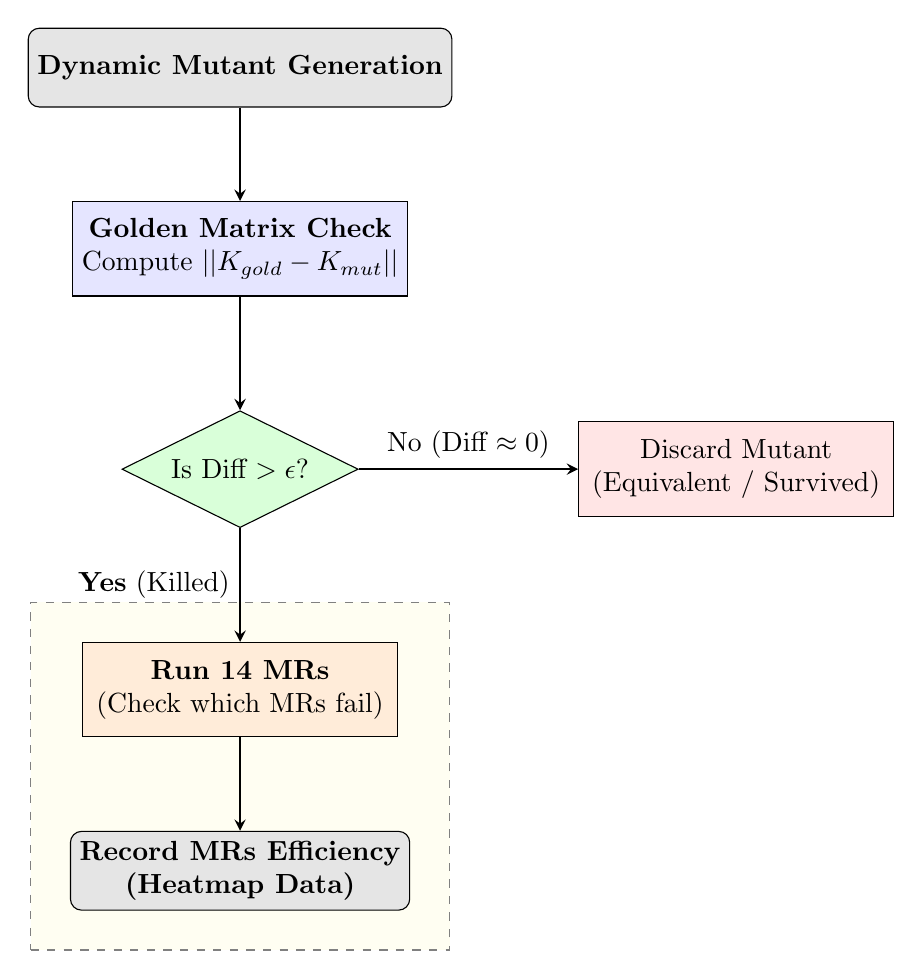
\begin{tikzpicture}[node distance=1.8cm]
			
			% --- STYLES ---
			\tikzstyle{startstop} = [rectangle, rounded corners, minimum width=3.5cm, minimum height=1cm, align=center, draw=black, fill=gray!20, font=\bfseries]
			\tikzstyle{process} = [rectangle, minimum width=4cm, minimum height=1.2cm, align=center, draw=black, fill=blue!10]
			\tikzstyle{decision} = [diamond, aspect=2, minimum width=3cm, minimum height=1cm, align=center, draw=black, fill=green!15]
			\tikzstyle{arrow} = [thick,->,>=stealth]
			\tikzstyle{line} = [draw, -latex']
			
			% --- NODES ---
			
			% 1. Start
			\node (gen) [startstop] {Dynamic Mutant Generation};
			
			% 2. Golden Matrix Step
			\node (golden) [process, below of=gen, yshift=-0.5cm] {
				\textbf{Golden Matrix Check}\\
				Compute $||K_{gold} - K_{mut}||$
			};
			
			% 3. Decision
			\node (decide) [decision, below of=golden, yshift=-1.0cm] {Is Diff $> \epsilon$?};
			
			% 4. Branch: Survived (Equivalent)
			\node (discard) [process, right of=decide, xshift=4.5cm, fill=red!10] {
				Discard Mutant\\
				(Equivalent / Survived)
			};
			
			% 5. Branch: Killed (Valid Bug) -> Evaluation
			\node (mr_suite) [process, below of=decide, yshift=-1.0cm, fill=orange!15] {
				\textbf{Run 14 MRs}\\
				(Check which MRs fail)
			};
			
			% 6. Final Result
			\node (output) [startstop, below of=mr_suite, yshift=-0.5cm] {
				Record MRs Efficiency\\
				(Heatmap Data)
			};
			
			% --- ARROWS ---
			\draw [arrow] (gen) -- (golden);
			\draw [arrow] (golden) -- (decide);
			
			% Yes Path (Vertical)
			\draw [arrow] (decide) -- node[anchor=east] {\textbf{Yes} (Killed)} (mr_suite);
			
			% No Path (Horizontal)
			\draw [arrow] (decide) -- node[anchor=south] {No (Diff $\approx 0$)} (discard);
			
			% Final
			\draw [arrow] (mr_suite) -- (output);
			
			% --- GROUPING BOX (Corrected Syntax) ---
			\begin{pgfonlayer}{background}
				\node[draw=black!50, dashed, fill=yellow!5, inner sep=0.5cm, fit=(mr_suite) (output), label={[text=gray!70, anchor=north west, xshift=1cm, yshift=-0.2cm]north west:\textit{}}] {};
			\end{pgfonlayer}
			
		\end{tikzpicture}
		\caption{Workflow for Measuring Metamorphic Relation Efficiency using the Golden Matrix Oracle}
		\label{fig:golden_matrix_flow}
	\end{figure}
	
	\subsection{Metamorphic Relations}
	
	\subsubsection{System-level Metamorphic Relations}
	\label{sec:sys_mrs}
	
	We defined five system-level metamorphic relations mathematically to assess the overall machine learning classification robustness. These relations are categorized in two groups as below:

		\begin{enumerate}
			\item \textbf{Scaling (MR\#1):} Multiplying all feature inputs by a constant scalar $c$
			\item \textbf{Rotation (MR\#2):} Rotating all features uniformly by a constant angle
			\item \textbf{Feature Permutation (MR\#3):} Swapping the index order of features uniformly across the entire dataset
			\item \textbf{Inverting Labels (MR\#4):} $y \to -y$. Reversing the classification labels in the data
			\item \textbf{Duplicating Data Inputs (MR\#5):} Adding identical rows to the dataset to test weighting stability
		\end{enumerate}
	
	In Figure \ref{fig:SVM_MRs}, we have the SVM related system-level metamorphic relations, which consists of four sub-figures. In Figure \ref{fig:sub-1-0}, QSVM classification is shown. With the first MR\#1 of scaling inputs, it is shown in Figure \ref{fig:sub-1-1} that the classification are not affected. Similarly with MR\#2, rotating all the inputs by the same angle will not affect the classification as. Furthermore, from MR\#3 to MR\#5, they are outlined in Figure \ref{fig:sub-1-2 }.
	
	
	\begin{figure}[H]
		\centering
		
		% --- FIRST ROW ---
		\begin{subfigure}{0.48\textwidth}
			\centering
			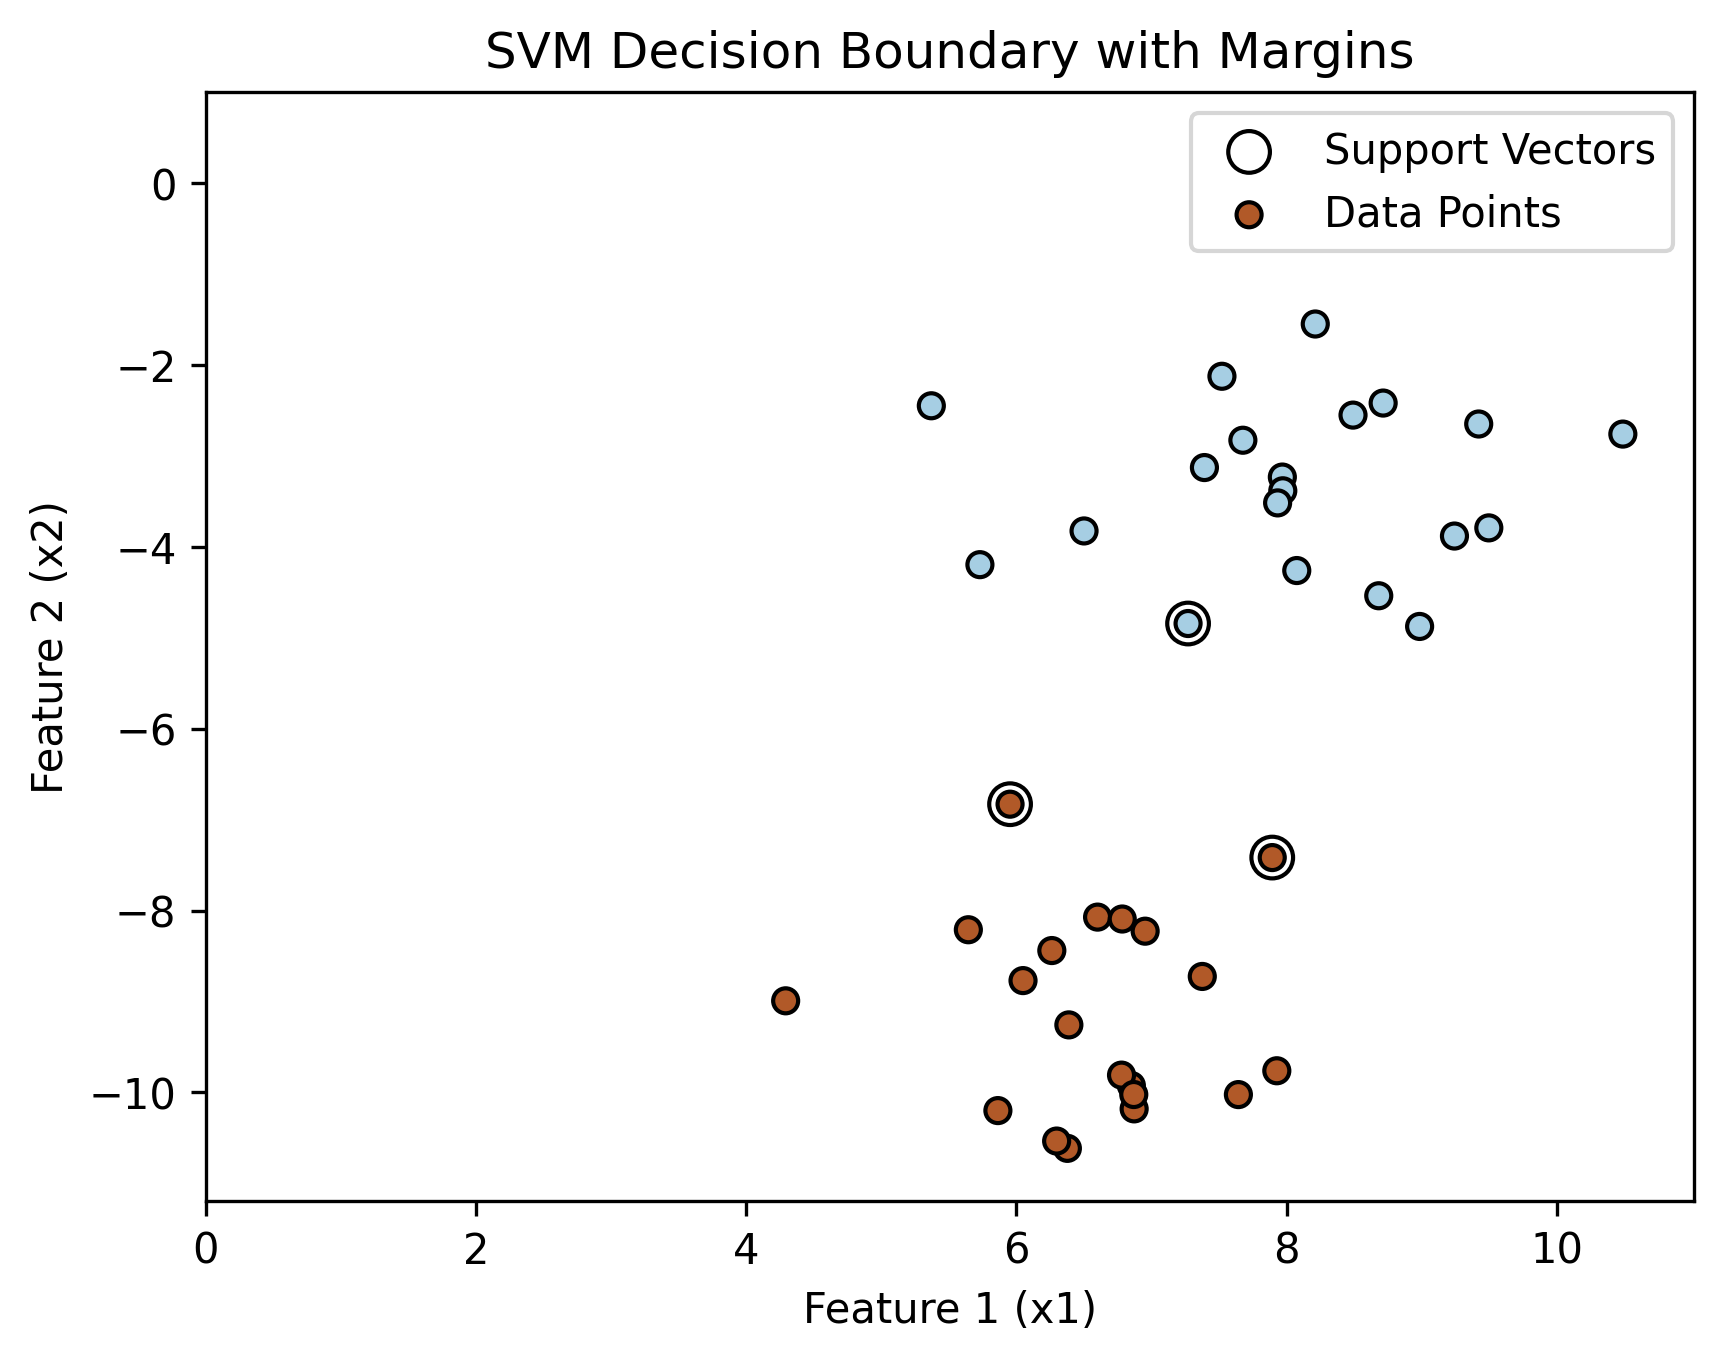
\includegraphics[width=\linewidth]{figures/original_plot.png}
			\caption{Original QSVM Classification}
			\label{fig:sub-1-0}
		\end{subfigure}%
		\hfill
		\begin{subfigure}{0.48\textwidth}
			\centering
			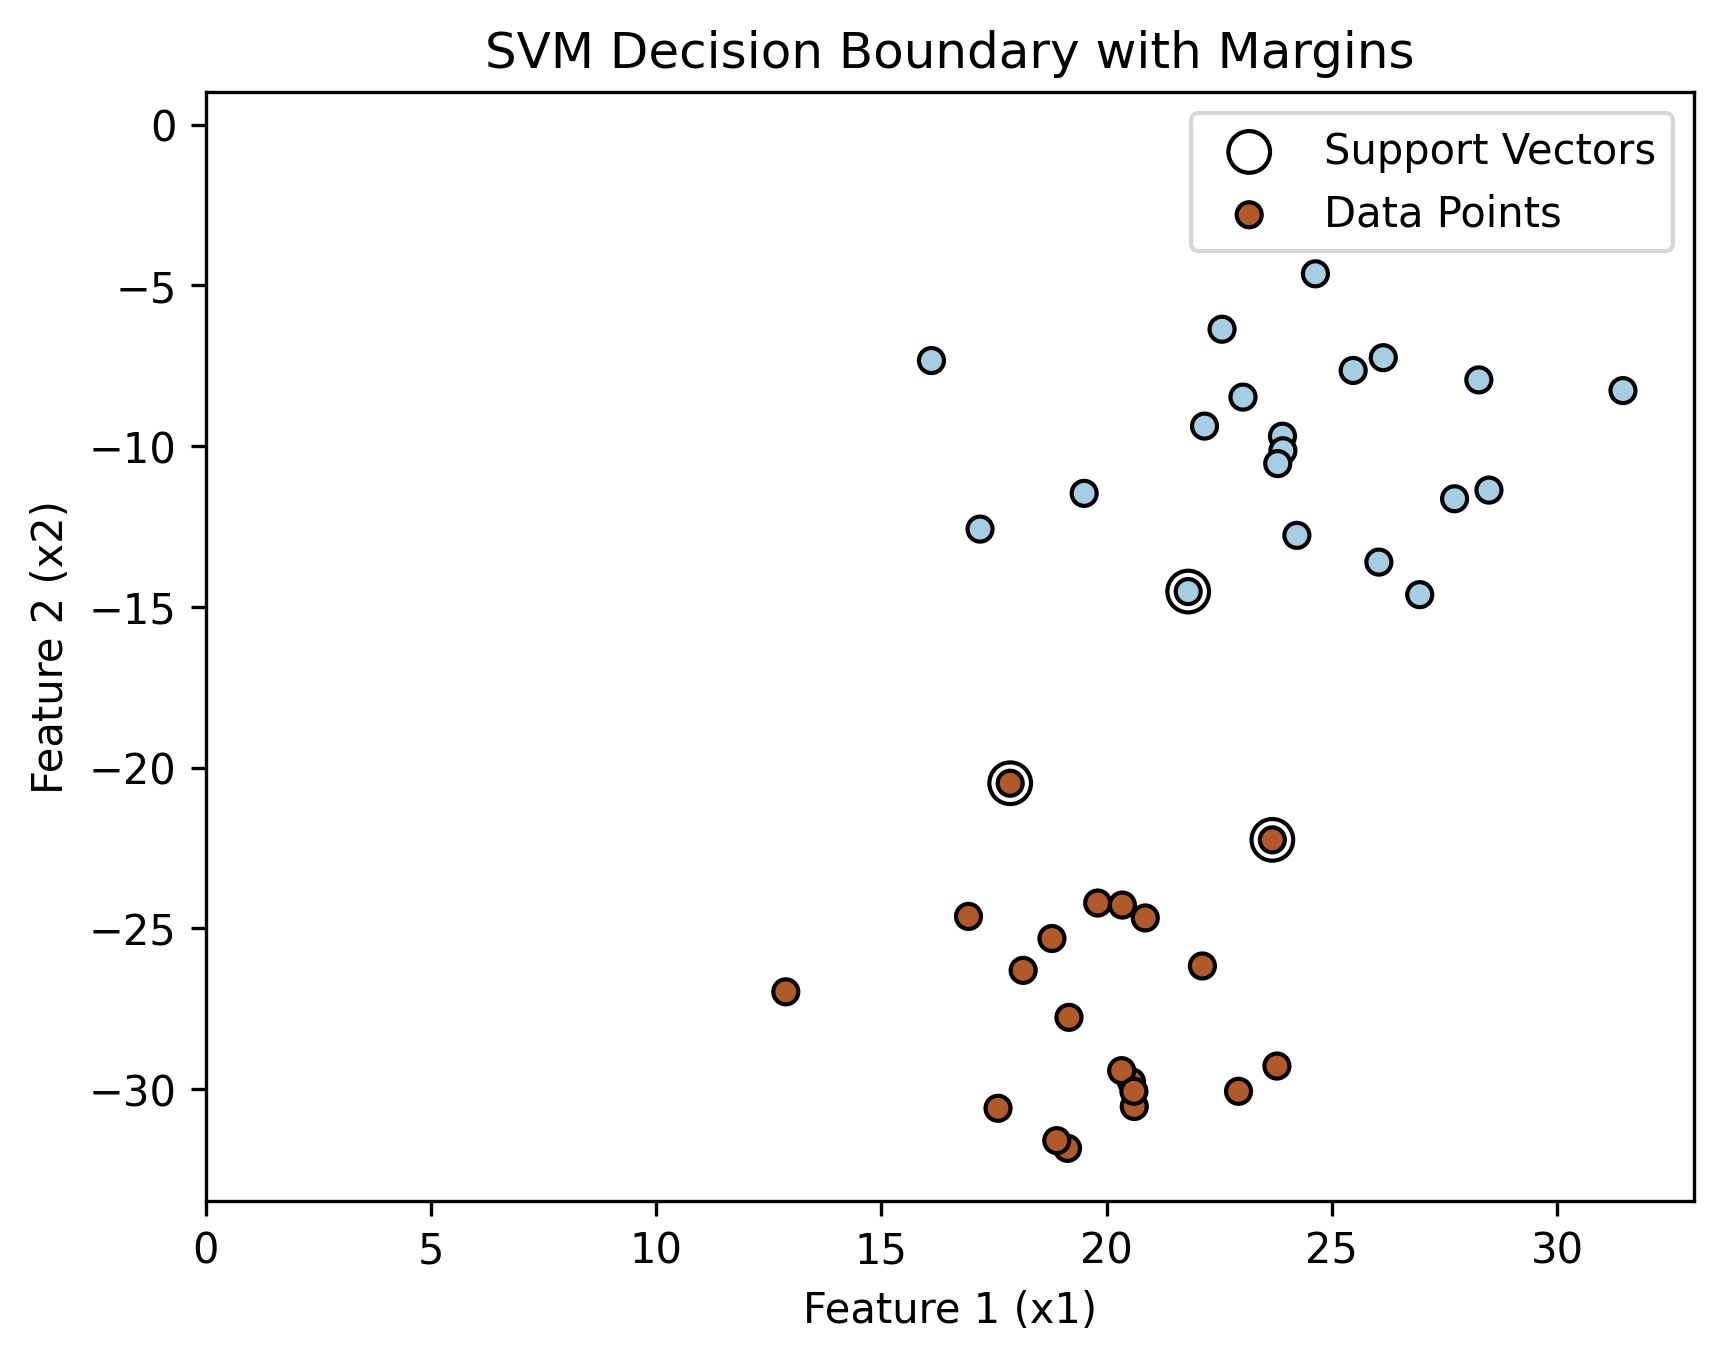
\includegraphics[width=\linewidth]{figures/mr_1_plot.png}
			\caption{QSVM Classification with MR\#1}
			\label{fig:sub-1-1}
		\end{subfigure}
		
		\vspace{1em} 
		
		% --- SECOND ROW ---
		\begin{subfigure}{0.48\textwidth}
			\centering
			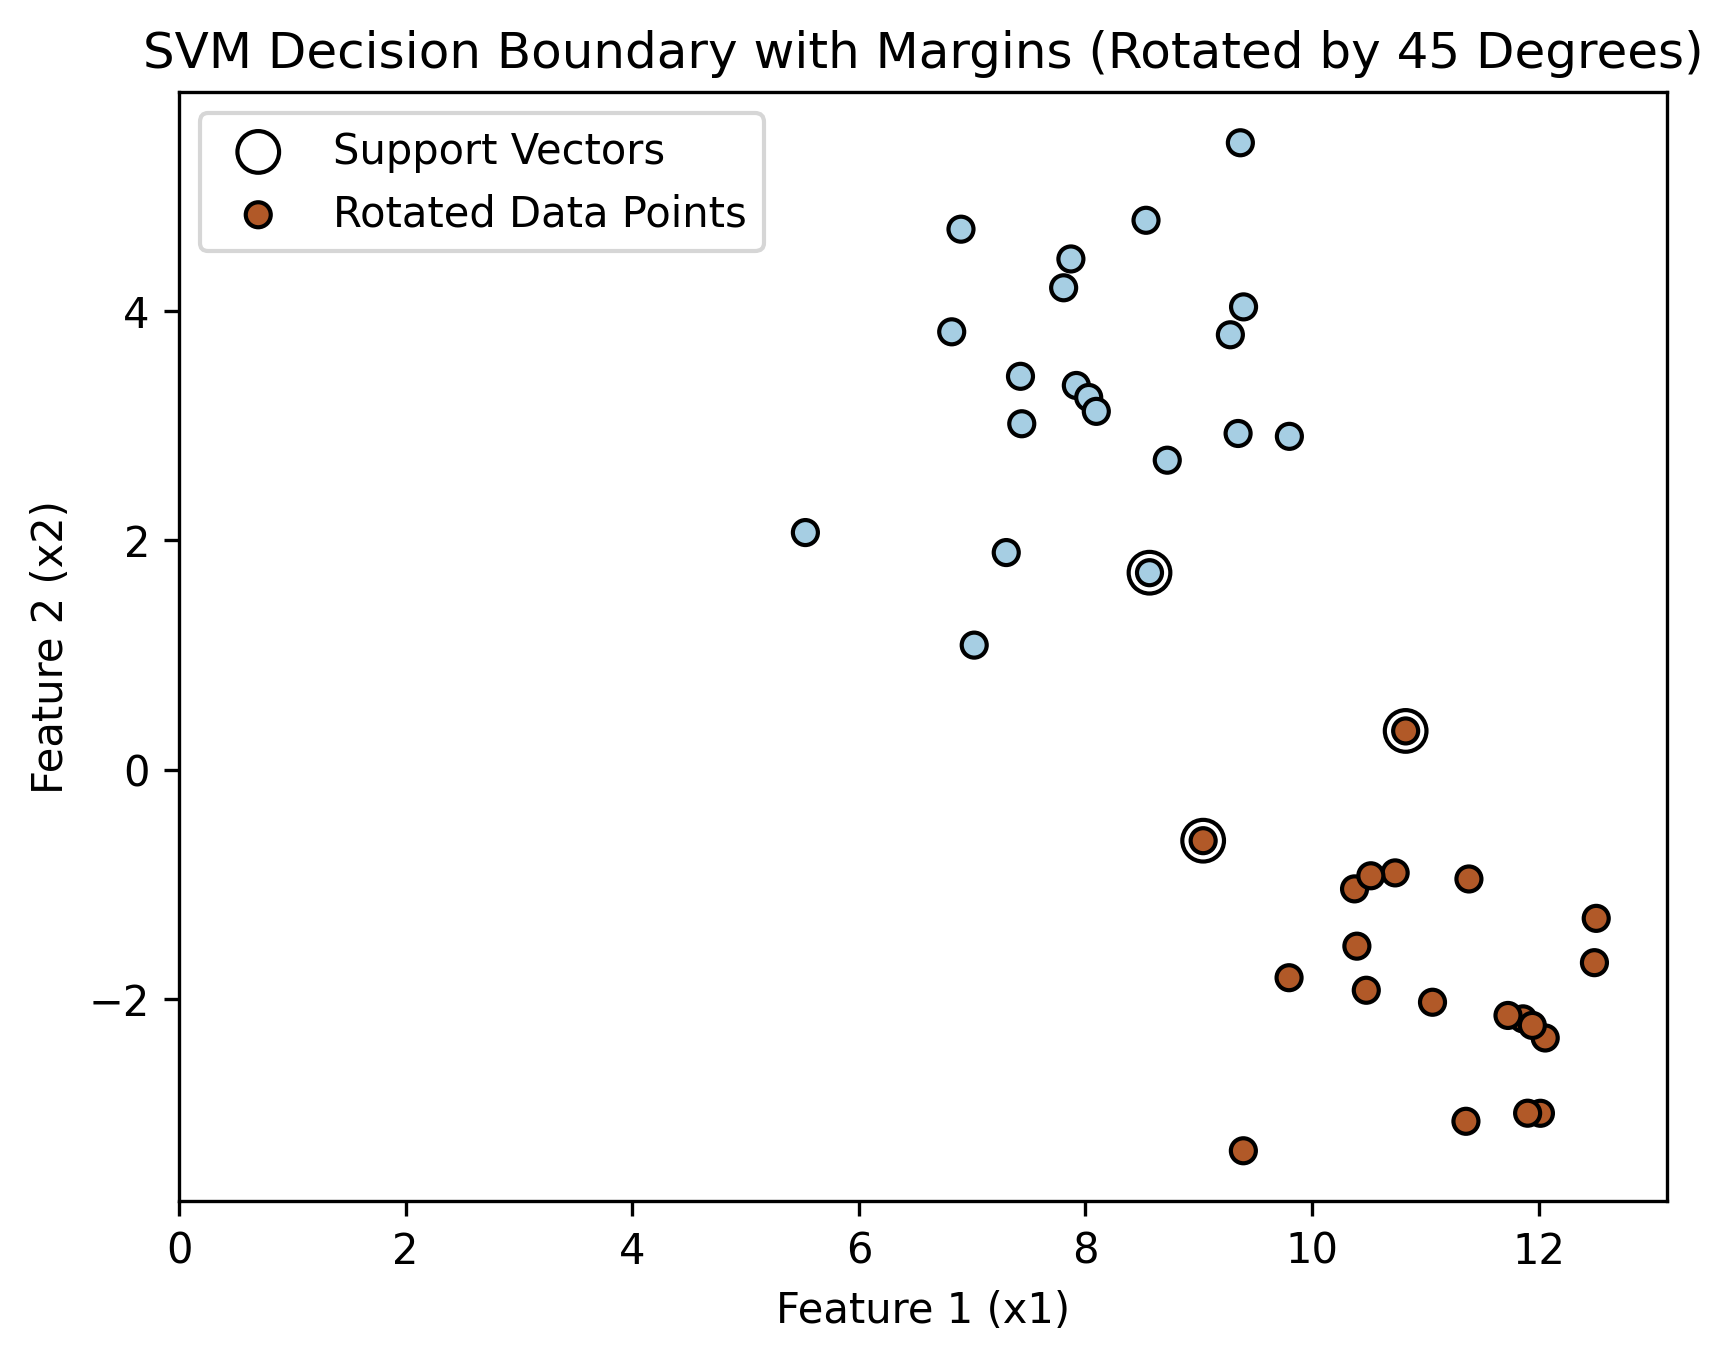
\includegraphics[width=\linewidth]{figures/mr_2_plot.png}
			\caption{QSVM Classification with MR\#2}
			\label{fig:sub-1-2}
		\end{subfigure}%
		\hfill
		\begin{subfigure}{0.48\textwidth}
			\centering
			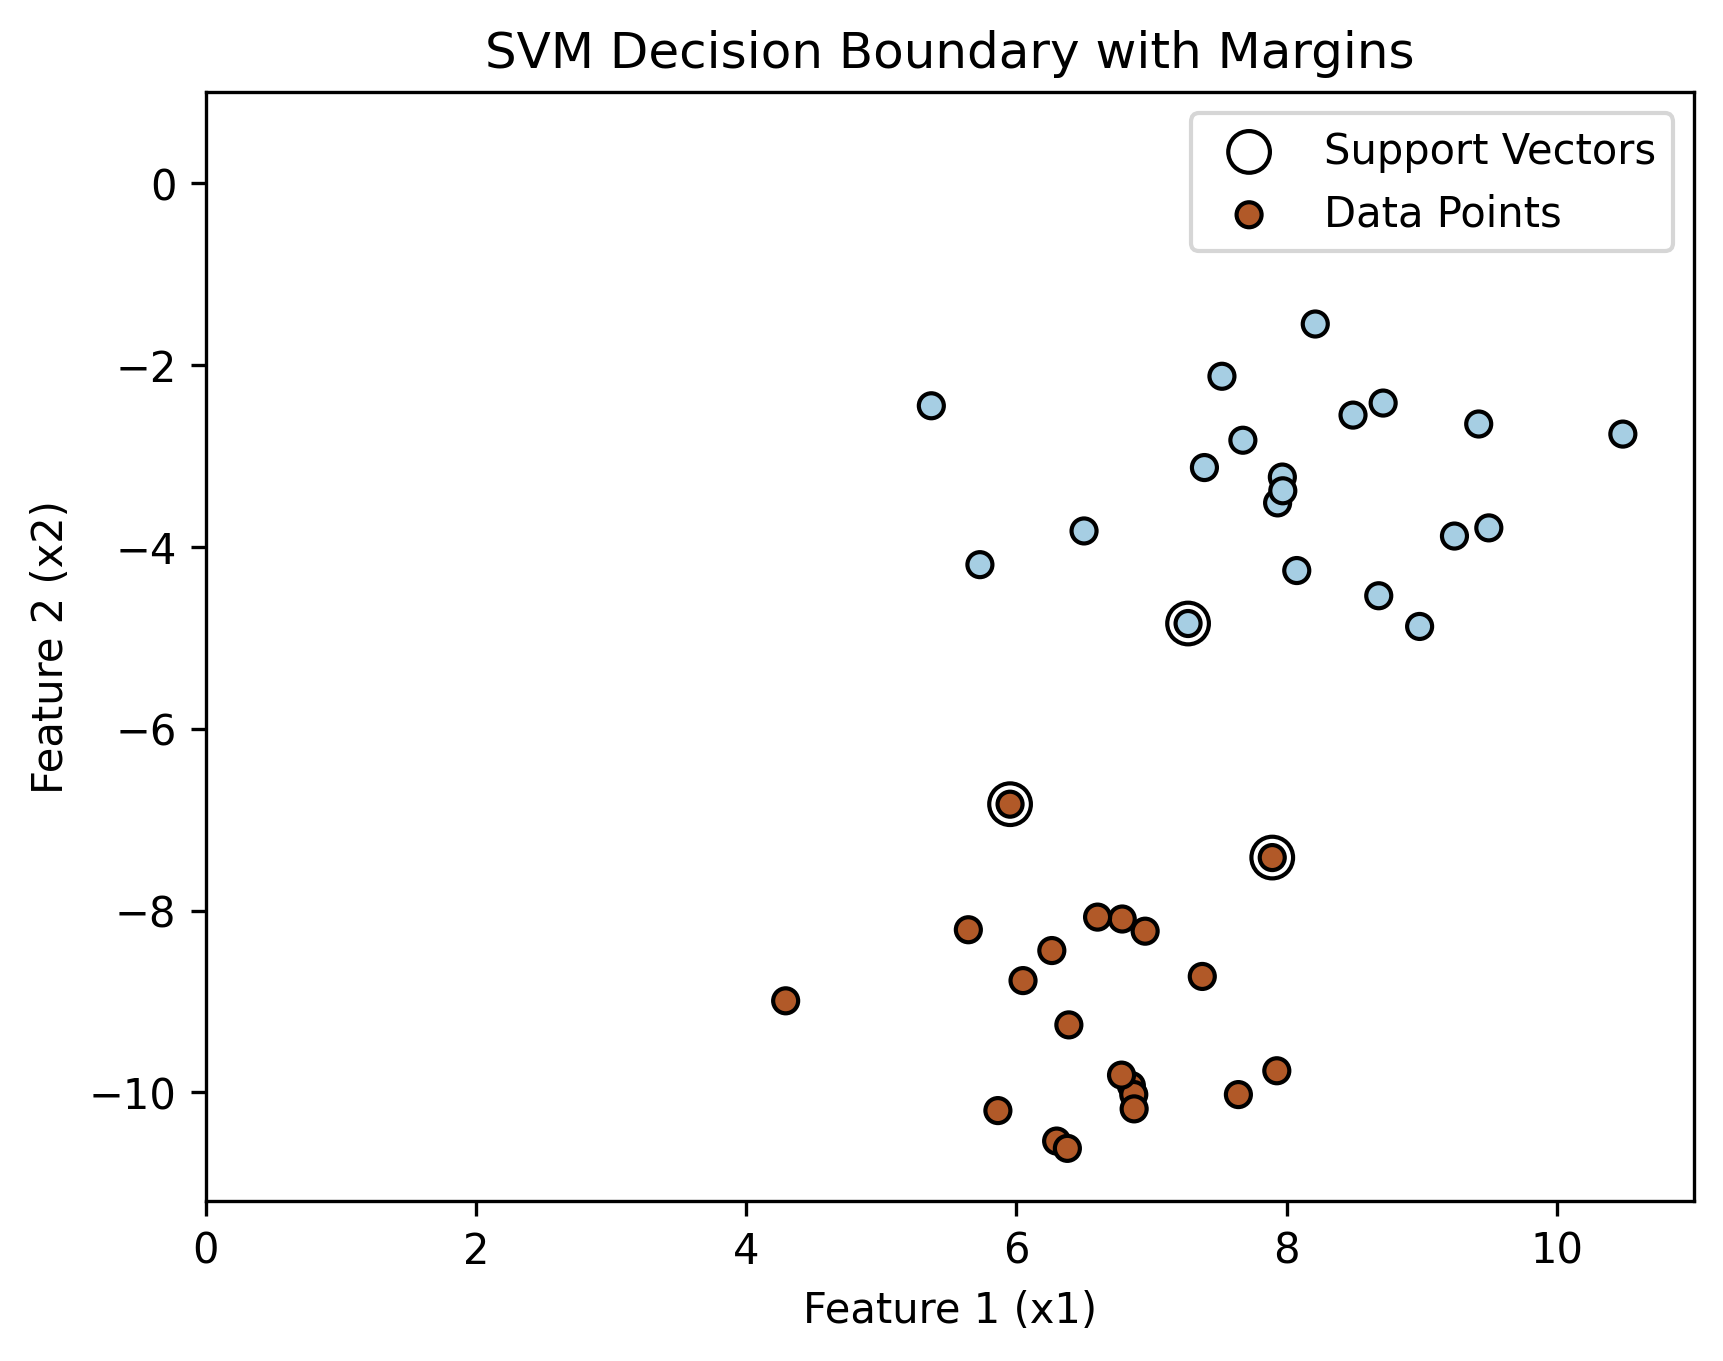
\includegraphics[width=\linewidth]{figures/mr_3_plot.png}
			\caption{QSVM Classification with MR\#3, MR\#4, and MR\#5 }
			\label{fig:sub-1-3}
		\end{subfigure}
		
		\caption{SVM Metamorphic Relations (MRs)}
		\label{fig:SVM_MRs}
	\end{figure}
	
		Additionally, the seven QC-related metamorphic relations applied at the system level are:

		\begin{enumerate}
			\setcounter{enumi}{5}
			\item \textbf{Add Quantum Register (MR\#6)}
			\item \textbf{Inject Null Effect Operations (MR\#7)}
			\item \textbf{Inject Parameters (MR\#8)}
			\item \textbf{Change of Testing Device (MR\#9)}
			\item \textbf{Change of Optimization Level (MR\#10)}
			\item \textbf{Reverse QC Wires (MR\#11)}
			\item \textbf{Switch Q-Kernel Inner Product Inputs (MR\#12)}
		\end{enumerate}
	
	
	In Figure \ref{fig:QC_MRs}, we display the angle embedding feature map and the metamorphic relations related to it as shown in the eight sub-figures. In Figure \ref{fig:sub-2-0}, the original circuit is shown. In Figure \ref{fig:sub-2-1}, the circuit original outcome should not be changed by adding an extra quantum register as a wire. In Figures \ref{fig:sub-2-2} and \ref{fig:sub-2-3}, adding two of the same gates in sequence or applying a general gate with an equivalent parameter respectively will result in the same functionality of the QC circuit. Then in Figure \ref{fig:sub-2-4}, it shows that changing the device to transpile an equivalent circuit does not change the process. Moreover, in Figure \ref{fig:sub-2-5}, changing the circuit optimization level as a metamorphic relation keeps the circuit the same. And when we reverse the QC wires as MR\#11 as shown in Figure \ref{fig:sub-2-7} or when we switch the inner product inputs for the quantum kernel, we are not changing the QSVM functionality which means that the classification outcome remains the same.
	
	\begin{figure}[!ht]
		\centering
		
		% --- Third ROW ---
		\begin{subfigure}{0.48\textwidth}
			\centering
			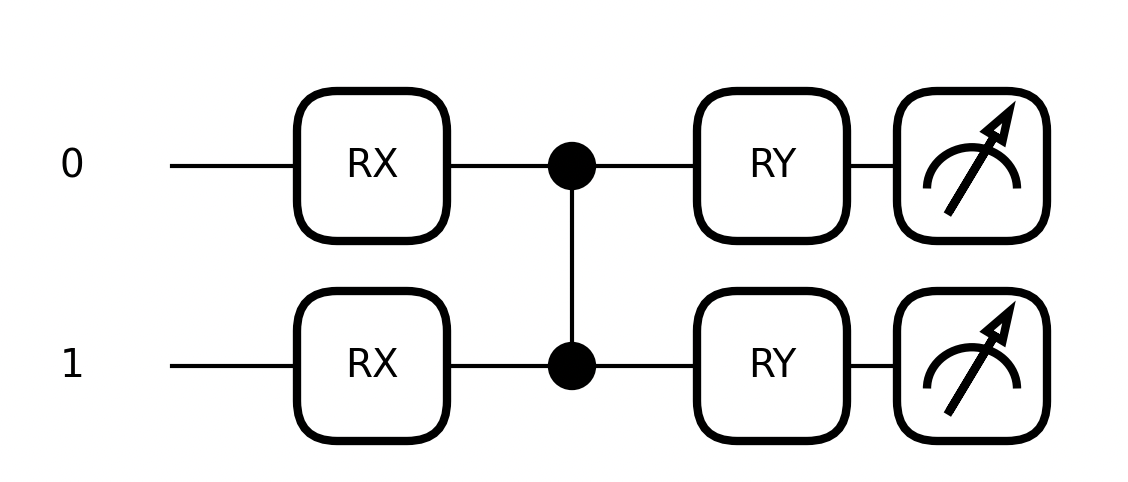
\includegraphics[width=\linewidth]{figures/qkernel2_original.png}
			\caption{ Feature Map}
			\label{fig:sub-2-0}
		\end{subfigure}%
		\hfill
		\begin{subfigure}{0.48\textwidth}
			\centering
			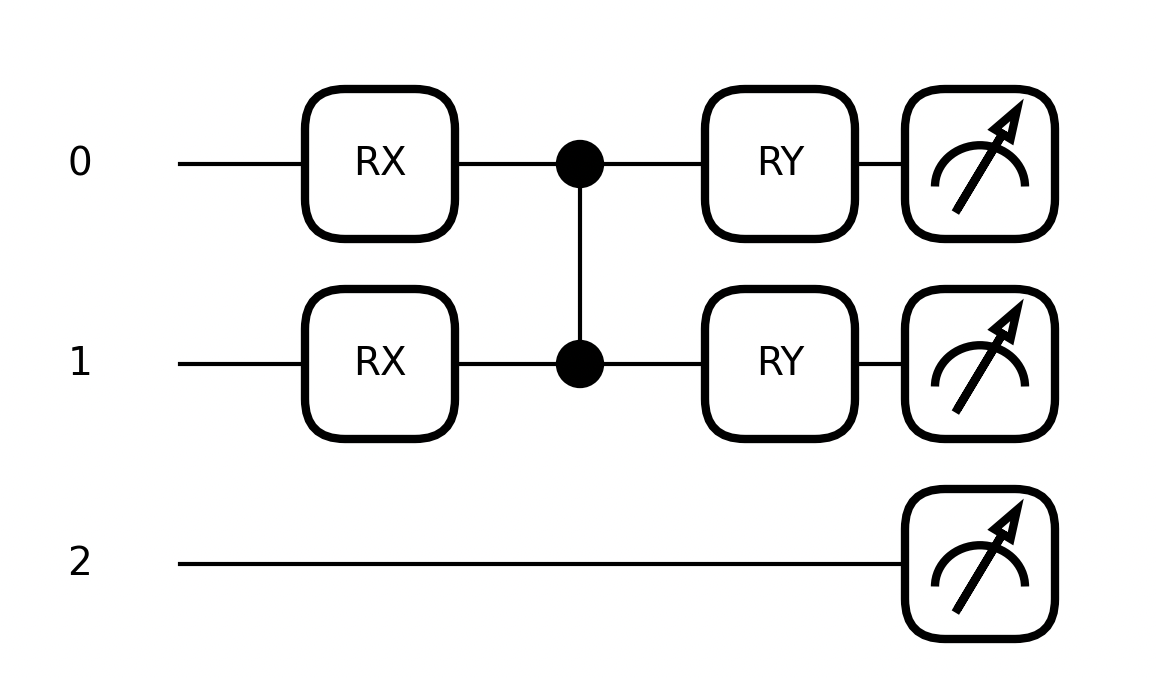
\includegraphics[width=\linewidth]{figures/qkernel2_mr6.png}
			\caption{Add Quantum Register (MR\#6)}
			\label{fig:sub-2-1}
		\end{subfigure}
		
		\vspace{1em} 
		
		% --- FOURTH ROW ---
		\begin{subfigure}{0.48\textwidth}
			\centering
			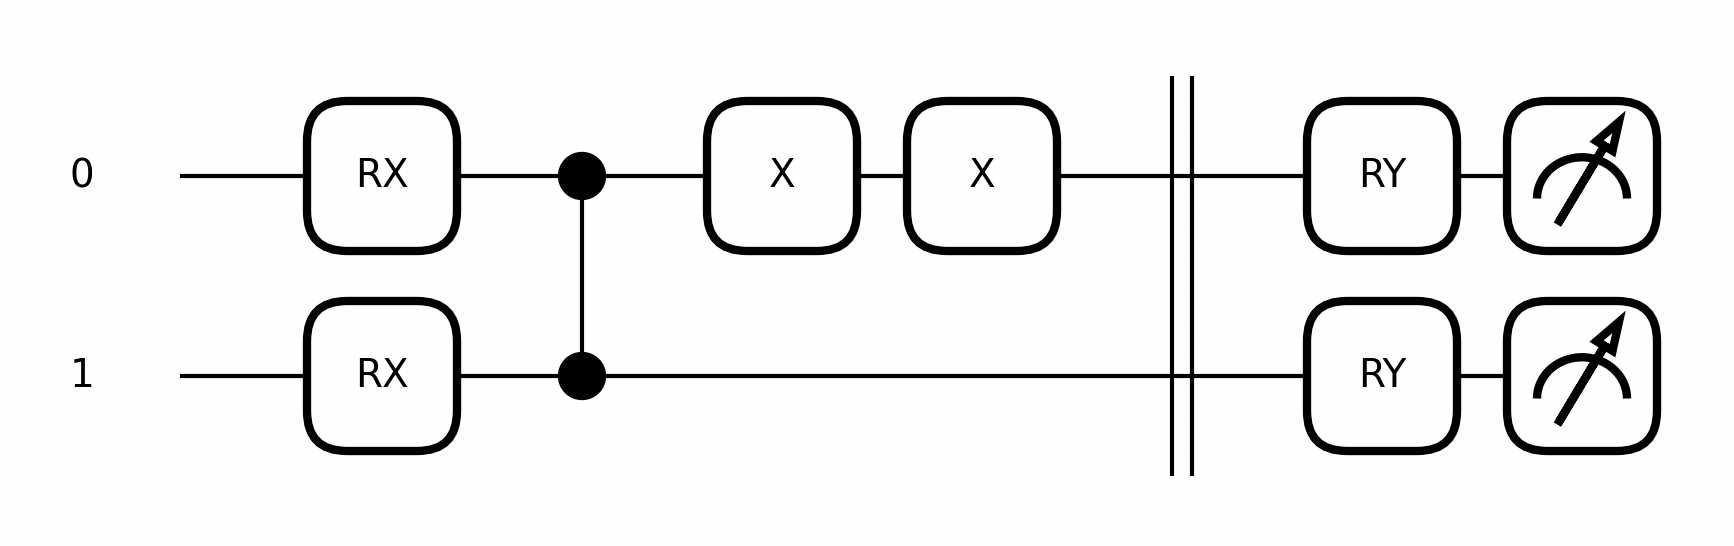
\includegraphics[width=\linewidth]{figures/qkernel2_mr7.png}
			\caption{ Inject Null Effect Operations (MR\#7)}
			\label{fig:sub-2-2}
		\end{subfigure}%
		\hfill
		\begin{subfigure}{0.48\textwidth}
			\centering
			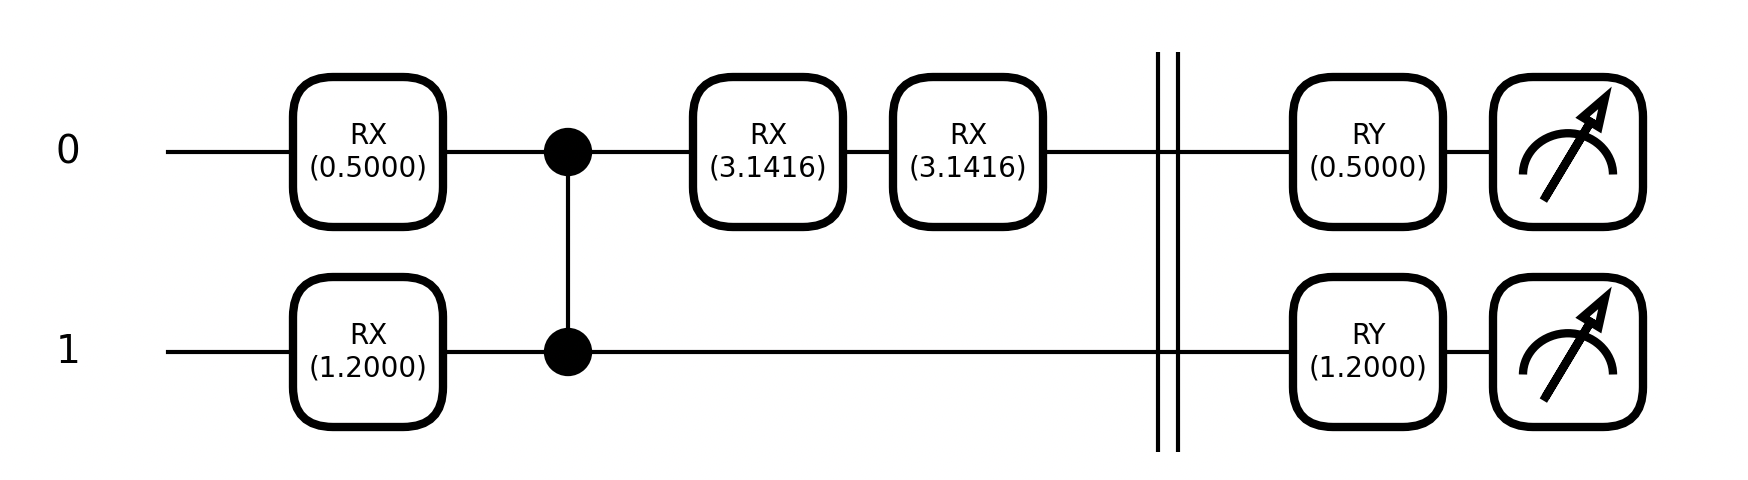
\includegraphics[width=\linewidth]{figures/qkernel2_mr8.png}
			\caption{Inject Parameters (MR\#8)}
			\label{fig:sub-2-3}
		\end{subfigure}
		
		\vspace{1em} 
		
		% --- FIFTH ROW ---
		\begin{subfigure}{0.48\textwidth}
			\centering
			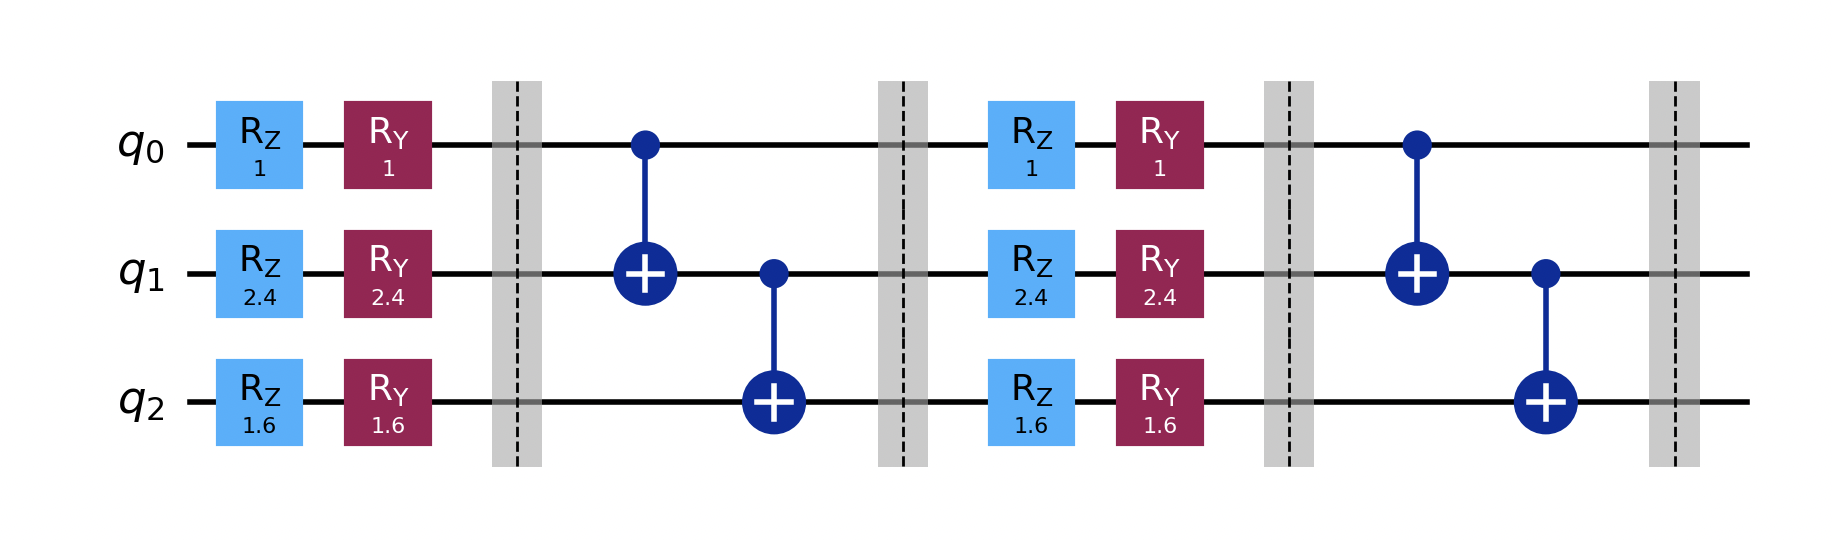
\includegraphics[width=\linewidth]{figures/qkernel2_mr9.png}
			\caption{ Change of Testing Device (MR\#9)}
			\label{fig:sub-2-4}
		\end{subfigure}%
		\hfill
		\begin{subfigure}{0.48\textwidth}
			\centering
			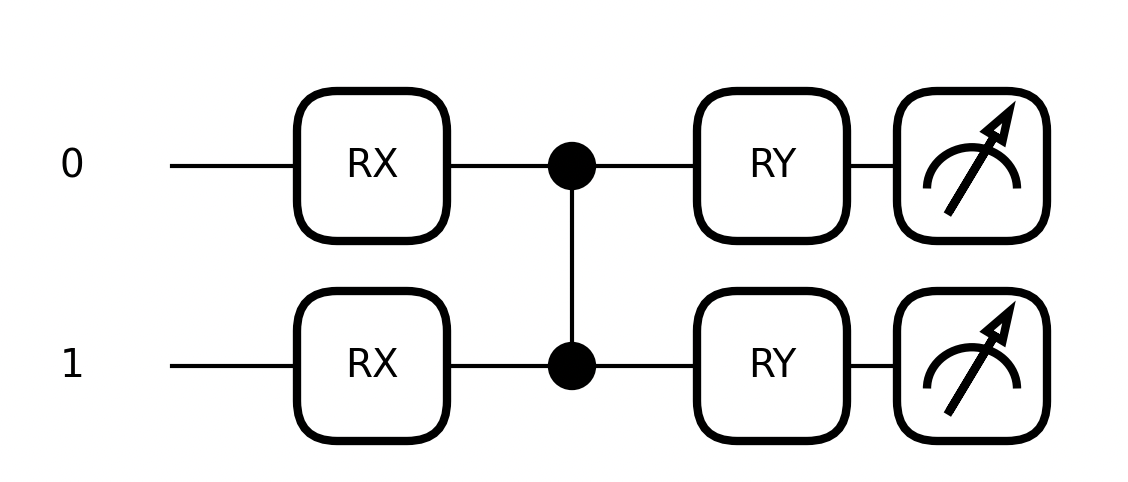
\includegraphics[width=\linewidth]{figures/qkernel2_mr10.png}
			\caption{Change of Optimization Level (MR\#10)}
			\label{fig:sub-2-5}
		\end{subfigure}
		
		\vspace{1em} 
		
		% --- SIXTH ROW ---
		\begin{subfigure}{0.48\textwidth}
			\centering
			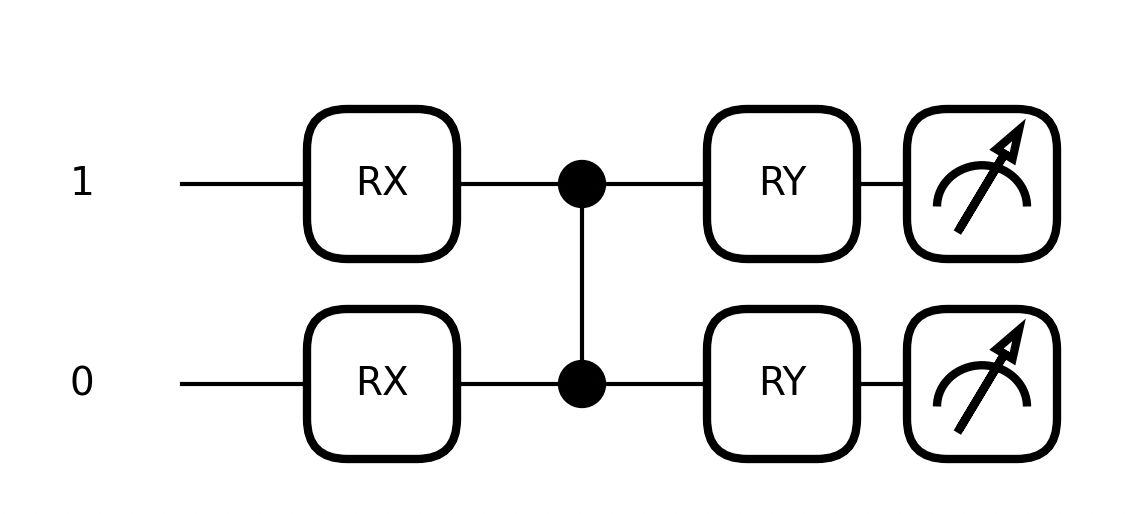
\includegraphics[width=\linewidth]{figures/qkernel2_mr11.png}
			\caption{ Reverse QC Wires (MR\#11)}
			\label{fig:sub-2-7}
		\end{subfigure}%
		\hfill
		\begin{subfigure}{0.48\textwidth}
			\centering
			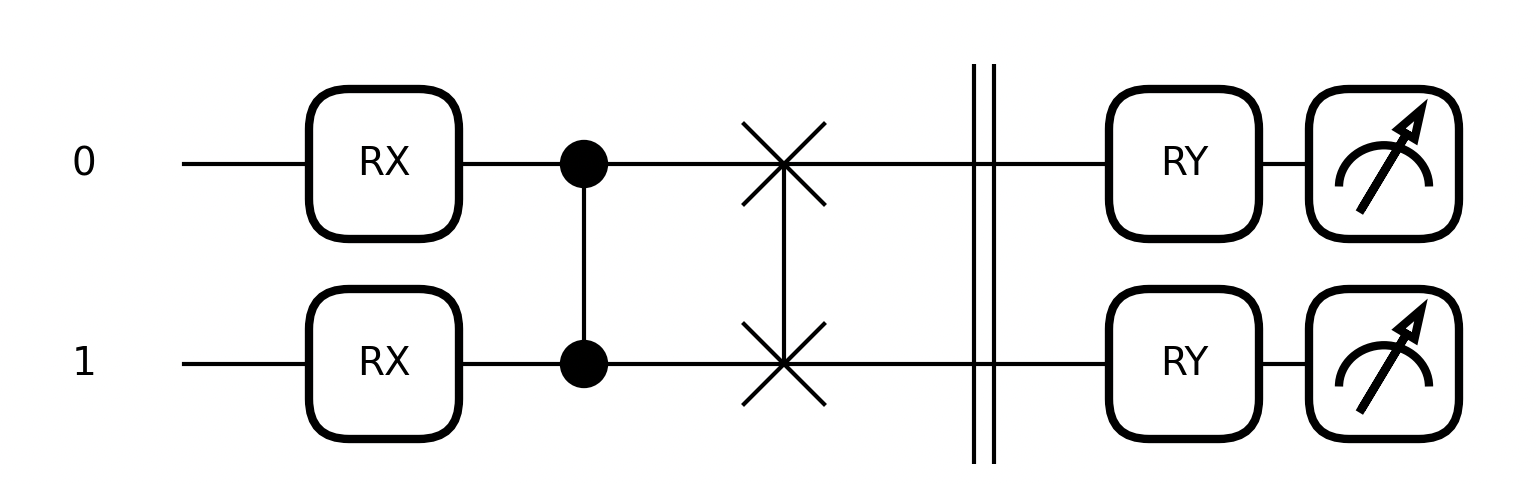
\includegraphics[width=\linewidth]{figures/qkernel2_mr12.png}
			\caption{Switch Q-Kernel Inner Product Inputs (MR\#12)}
			\label{fig:sub-2-8}
		\end{subfigure}
		
		\caption{QC Metamorphic Relations (MRs)}
		\label{fig:QC_MRs}
	\end{figure}
	
	\subsubsection{Kernel-Level Metamorphic Relations}
	\label{sec:kernel_mrs}
	
	Transitioning to the quantum kernel, we identified 14 kernel-level Metamorphic Relations to targeting the target kernel evaluation. They are divided into three validation groups:
	
	\paragraph{Group A: General Mathematical Relations}
	These are based on the properties of inner product and kernels, which are implementation independent \cite{schuld2019}.
	\begin{itemize}
		\item \textbf{MR1 (Symmetry)}: $K(x,y) = K(y,x)$ 
		\item \textbf{MR2 (Identity)}: $K(x,x) = 1$
		\item \textbf{MR7 (Permutation)}: Invariant to the simultaneous shuffling of features in both input vectors \cite{xie2011}
	\end{itemize}
	
	\paragraph{Group B: Quantum-Specific Relations}
	These relations adopt the concept of Quantum metamorphic relations defined in the MorphQ framework \cite{Paltenghi2023}. They target properties unique to quantum circuits.
	
	\begin{itemize}
		\item \textbf{MR9 (Noise Stability)}: Evaluates robustness against small input perturbations; small $\epsilon$ shifts in $x$ should not cause divergent kernel values
		\item \textbf{MR12 (Structural Orthogonality)}: Verifies that orthogonal quantum states remain non-overlapping \cite{schuld2019}: $K(x, x_{\perp}) \approx 0$
		\item \textbf{MR13 (Dual Consistency)}: Validates that reversing the input feature order $K(rev(x), rev(y))$ maintains the same relationship as $K(x, y)$, testing the consistency of the entanglement chain \cite{Paltenghi2023}
		\item \textbf{MR14 (Qubit Permutation)}: Ensures that changing the physical qubit mapping (wire map) does not alter the kernel output \cite{Paltenghi2023}
	\end{itemize}
	
	\paragraph{Group C: Feature-Embedding Specific Relations}
	These relations are valid only for specific data embedding strategies—Basis, Angle, and Amplitude—which dictate the algorithm's specific symmetries \cite{zaman2025surveyquantummachinelearning, schuld2018}
	\begin{itemize}
		
		\item \textbf{MR4 (Shift Invariance)} \cite{havlicek2019}:  $K(x+c, y+c) \approx K(x,y)$ 
		
		\item \textbf{Angle Embedding Specific (MR5))} Exploits the periodicity property in rotational gates \cite{Sweke2020, havlicek2019}: $K(x+2\pi, y) \approx K(x,y)$
		
		\item \textbf{Basis Embedding Specific MR8 (Bit Inversion)}: $K(1-x, 1-y) \approx K(x,y)$ Targets bit-wise logic used in computational basis encoding \cite{Dwarakanath2018}
		
		\item \textbf{MR11 (Linear Scaling)}: $K(cx, cy) \approx K(x,y)$ (Amplitude only) \cite{mottonen2004}
		
		\item \textbf{Common}:
		\begin{itemize}
			\item \textbf{MR3 (Negation)}: $K(-x,-y) \approx K(x,y)$ \cite{xie2011}
			
			\item \textbf{MR6 (Feature Rotation):} Invariant to cyclic feature shifts \cite{LaRose2020}
			
			\item \textbf{MR10 (Feature Sensitivity)}: Metamorphic Change. Zeroing out a feature must change the kernel value \cite{Segura2016}
			
		\end{itemize}
	\end{itemize}

	
	\section{Evaluating the Effectiveness of Metamorphic Relations}
	\label{sec:evaluation}
	
	\subsection{Research Questions}
	
	There are some research questions that inspired this work, and they are:
	\begin{itemize}
		\item RQ1: What are the most effective metamorphic relations (MRs) for testing Quantum Support Vector Machines?
		\item RQ2: How well will the metamorphic relations used with SVM perform with Quantum Support Vector Machines?
		\item RQ3: How stochastic is QSVM and does QSVM require statistical testing?
		\item RQ4: How efficient will be metamorphic testing if applied only on the quantum kernel?
	\end{itemize}
	
	\subsection{Methodology}
	
	In our experiment, we adopted statistical testing with system-level metamorphic testing, as shown in Figure \ref{fig:3}, to determine whether there were any coincidental differences between the models and to ensure there were no randomness \cite{10.1145/1985793.1985795} in the experiment. The metamorphic Testing Score is calculated as the following:
	
	\[
	\text{IsNonEqual}(M, (\bar{M_{0,0,0}}, \ldots, \bar{M_{K,J,V}}),\  x_{test}^i)) =
	\begin{cases} 
		\text{false} & \text{if } y^i_{test} = y^i_{pre} 
		\\
		\text{true} & \text{otherwise}
	\end{cases}
	\]
	
	\begin{equation}
		\label{eq:MTS}
		MTS =  \frac{\{y^i_{test} \in y_{test},\ {\bar{M}} \in \bar{MS} \mid \text{isNonEqual} \ (M, (\bar{M_{0,0,0}}, \ldots, \bar{M_{K,J,V}}),\  x_{test}^i)\}}{\mid \bar{MS} \mid * \mid y_{test} \mid} 
	\end{equation}
	
	Where $y^i_{test}$ is the testing data, $M$ is the model, and $\bar{M}$ is the modified data model. There are three factors to differentiate between the modified data models. First factor is $k$ that represents which k-fold data was used. Second factor is $j$ that represents which metamorphic relation (MR) is used, and $v$ that represents what value is used with the metamorphic relation. For example, if we pick k-fold of value 1,  MR of value 1 which is multiplying all the data by a scalar of value $v$ and the picked scalar value was 5, then the model will be named as $M_{11,1,5}$. $x^i_{test}$ represents the inputs and $\mid \bar{MS} \mid$ is the number of all models. The MTS should be equal to 0 which indicates that no bugs were found in the implementation of QSVM. The p-value shows if the null hypothesis is more likely or the alternative hypothesis. In our experiment, the p-value threshold is $0.05$ and has to be bigger than that to support the null hypothesis $H_0$) states that there is no statistically significant difference between the accuracy of the original data and the modified data. The alternative hypothesis ($H_1$) states that a statistically significant difference exists.
	
	Furthermore, we initially adopted noise factors in the experiment with system-level MRs to simulate real quantum computing noise, and we had four different types of noise to be implemented in Pennylane as follows:
	\begin{itemize}
		\item Depolarizing Channel Noise
		\item Bit-flip noise
		\item Amplitude Damping Noise
		\item Phase Damping Noise
	\end{itemize}
	
	However, it was found out that adding noise to the experiment did not make it deterministic. This is because the noise was propagating through the density matrix before the measurements. We ended up relying on adding more shots to the experiment to simulate randomness in randomness instead. More details will be in the Results section (\ref{sec:results}).
	
	\subsection{Implementation}
	\label{sec:implementation}
	
	For platform and libraries, we selected Qiskit SDK and Pennylane library. Both of them are tools that can be used with the Python programming language. First, the reason for selecting Python is because it is the most well-known programming language for AI development, and also for QC development. Moreover, Pennylane is an emerging library that facilitates working with QML algorithms.
	
	A modular approach was incorporated in the development to allow the code to be reused with different components and aspects in the future. For example, instead of working on just QSVM, the work can be extended to deep learning algorithms like neural networks. In Figure \ref{fig:2}, we can see how the QSVM is established. We have five different types of datasets of different dimensions (number of features), number of labels (classifications) and the number of inputs in each one of them varies as well as shown below in Table \ref{tab:Datasets}.
	
	\begin{table}[h!]
		\centering
		\begin{tabular}{|c|c|c|c|}
			\hline
			\textbf{Data} & \textbf{Inputs} & \textbf{Dimension} & \textbf{labels}\\ \hline
			Wine Data             & 178            & 13      & 3              \\ \hline
			Load Digits            & ~1800             &64        & 10          \\ \hline
			Credit Card           & ~284,000             &30           & 2       \\ \hline
			MNIST               & 70,000             & 784         & 10        \\ \hline
			custom               & any              & any          & any      \\ \hline
		\end{tabular}
		\caption{Datasets}
		\label{tab:Datasets}
	\end{table}
	
	\begin{figure}[t!]
		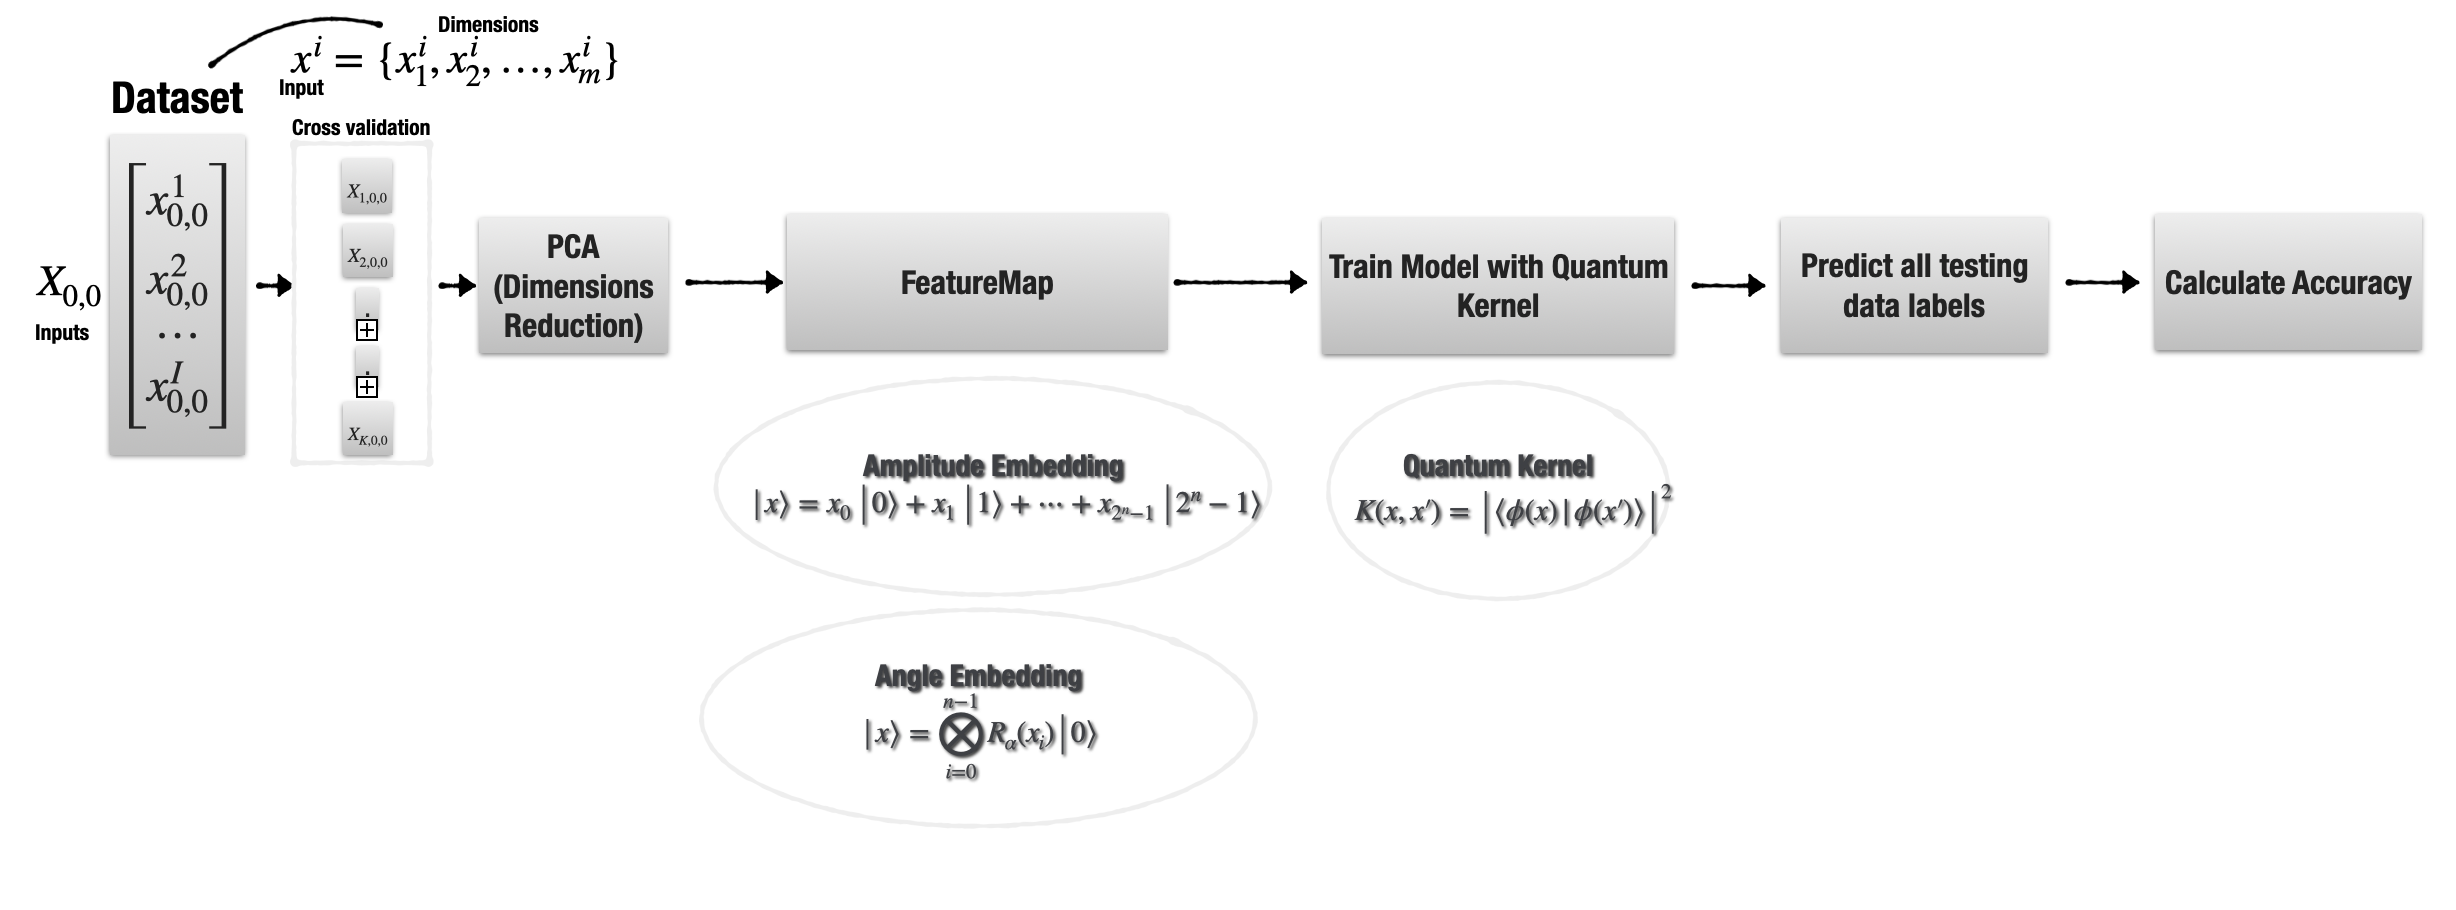
\includegraphics[height = 6.2 cm ,width=\linewidth]{figures/figure_1.png}
		\caption{QSVM}
		\label{fig:2}
	\end{figure}
	
		\begin{figure}[t!]
		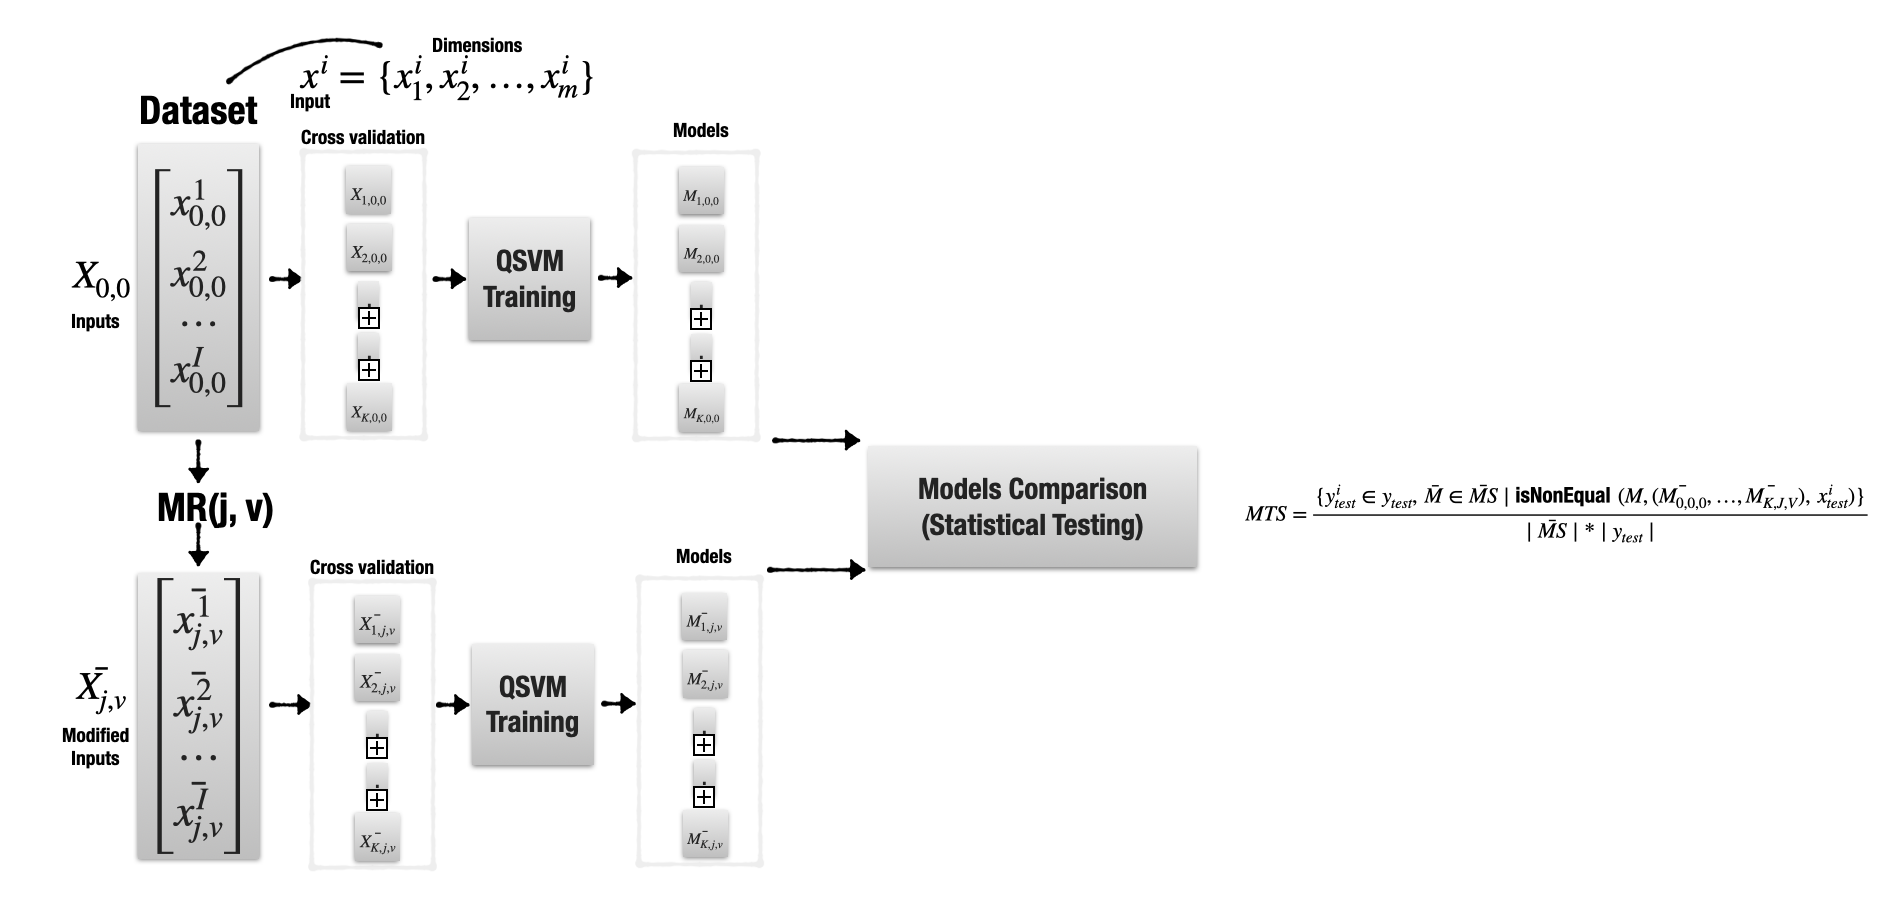
\includegraphics[height = 6.2 cm ,width=\linewidth]{figures/figure_2.png}
		\caption{QSVM with Statistical testing}
		\label{fig:3}
	\end{figure}
	
	The QSVM, as shown in Figure \ref{fig:2}, takes any dataset and applies cross-validation to ensure that the ML training is generalized and to avoid any potential over-fitting that might occur. Afterwards, optionally Principal Component Analysis (PCA) can be applied to reduce the data dimensions, i.e., the number of features. Then before using QSVM quantum kernel, we need to map the classical inputs to qubits. This can be done using a feature map. We have used two types of feature maps in system-level metamorphic testing, which are: amplitude embedding and angle embedding. These are two most generic feature maps \cite{10493306}, and there are others like the ZZ feature map \cite{havlicek2019}, which is based on angle embedding feature map and can be used in future along with other feature maps. In amplitude embedding, the classical inputs are encoded in the quantum amplitude. If we have a given feature vector $\mathbf{x} \in \mathbb{R}^n$, the \textit{feature amplitude embedding} $\Phi: \mathbb{R}^n \to \mathbb{C}^m$ maps the features to a complex-valued space where amplitudes encode feature information:
	
	\begin{equation}
		\Phi(\mathbf{x}) = \sum_{i=1}^{n} x_i \psi_i
	\end{equation}
	
	where:
	\begin{itemize}
		\item $x_i$ are the components of the feature vector $\mathbf{x}$
		\item $\psi_i \in \mathbb{C}^m$ are basis vectors with $|\psi_i| = 1$
		\item The amplitude $|x_i|$ represents the strength or importance of feature $i$
	\end{itemize}
	
	The embedding preserves feature relationships through the inner product structure:
	\begin{equation}
		\langle \Phi(\mathbf{x}), \Phi(\mathbf{y}) \rangle = \sum_{i,j} x_i y_j^* \langle \psi_i, \psi_j \rangle
	\end{equation}
	
	For orthogonal basis vectors ($\langle \psi_i, \psi_j \rangle = \delta_{ij}$), this simplifies to:
	\begin{equation}
		\langle \Phi(\mathbf{x}), \Phi(\mathbf{y}) \rangle = \mathbf{x} \cdot \mathbf{y} = \sum_{i=1}^n x_i y_i^*
	\end{equation}
	
	And in Angle embedding, given a feature vector $\mathbf{x} \in \mathbb{R}^n$, the \textit{angle embedding} $\Psi: \mathbb{R}^n \to \mathbb{C}^m$ maps features into a complex space where phase angles encode information while amplitudes remain fixed:
	
	\begin{equation}
		\Psi(\mathbf{x}) = \sum_{i=1}^{n} r_i e^{i \theta_i(x_i)} \psi_i
	\end{equation}
	
	where:
	\begin{itemize}
		\item $r_i \in \mathbb{R}^+$ is a constant amplitude (often $r_i = 1$)
		\item $\theta_i(x_i)$ is a phase encoding function (e.g., $\theta_i(x_i) = \pi x_i$ or another nonlinear mapping)
		\item $\psi_i \in \mathbb{C}^m$ are basis vectors (typically orthonormal: $\langle \psi_i, \psi_j \rangle = \delta_{ij}$)
	\end{itemize}
	
	The inner product between two angle-embedded vectors reflects their angular similarity:
	\begin{equation}
		\langle \Psi(\mathbf{x}), \Psi(\mathbf{y}) \rangle = \sum_{i=1}^{n} r_i^2 e^{i (\theta_i(x_i) - \theta_i(y_i))}
	\end{equation}
	
	Then, the quantum kernel $K: \mathbb{R}^d \times \mathbb{R}^d \to \mathbb{R}$ measures the overlap between two feature-embedded states:
	
	\begin{equation}
		K(\mathbf{x}_i, \mathbf{x}_j) = \left| \bra{\phi(\mathbf{x}_i)} \ket{\phi(\mathbf{x}_j)} \right|^2
	\end{equation}
	
	This is equivalent to the probability of measuring the all-zero state after applying $U^\dagger(\mathbf{x}_j)U(\mathbf{x}_i)$:
	\begin{equation}
		K(\mathbf{x}_i, \mathbf{x}_j) = \left| \bra{0}^{\otimes n} U^\dagger(\mathbf{x}_j) U(\mathbf{x}_i) \ket{0}^{\otimes n} \right|^2
	\end{equation}
	
	
	After the data training is finished with the quantum kernel, we apply the testing data to calculate the model accuracy.
	
	To achieve sub-circuit mutation testing, we modified the code to be more expressive and explicit, and we have added a third feature map known as basis embedding to the test. Basis encoding maps binary inputs directly to the computational basis states of the qubits \cite{schuld2018}:
			$$ \mathbf{x} = \{x_1, x_2, \dots, x_N\} \in \{0,1\}^N \rightarrow |x_1 x_2 \dots x_N\rangle $$
		
		For the embeddings, we used explicit logic for the three feature maps to have more space for creating mutants. The code is outlined in Listing \ref{lst:qsvmHealthyCode}
	
	\begin{lstlisting}[caption=Standard QSVM Script (Explicit Embedding Logic), label={lst:qsvmHealthyCode}]
		#Basis Embedding
		if mode == "basis":
		for i in range(len(x)):
		if x[i] > 0.5: 
		qml.PauliX(wires=wires[i])
		
		#Angle Embedding
		elif mode == "angle":
		for i in range(len(x)):
		qml.RY(x[i], wires=wires[i])
		
		#amplitude Embedding		
		elif mode == "amplitude":
		layers = get_angles(x)
		qml.RY(layers[0][0], wires=wires[0])
		for i in range(1, len(layers)): 
		ur_cnot(layers[i], wires[:i], wires[i])
	\end{lstlisting}
	
	Moreover,  have transitioned from creating mutations manually to a dynamic approach for creating mutations, and we categorized the mutations in three classes to line up with the literature of mutations generation \cite{9844849, qMutphyFortunato}:
	\begin{itemize}
		\item Data Level: Injecting Noise
		\item Gate Level: 
		\begin{itemize}
			\item  Flips the bit value (Pauli-X)
			\item Skips the gate operation within explicit loop
			\item Skips the Hadamard initialization for superposition
			\item Replaces the recursive CNOT logic with local rotations, to remove the entanglement
		\end{itemize}
		\item Structural Level: Switch between control qubit and target qubit to change the topology
	\end{itemize}
	
	The mutation logic is applied and shown in Listing \ref{lst:mutationClass}.
	
	
	
	\begin{lstlisting}[caption=Dynamic Mutator Sample, label={lst:mutationClass}]
		class AutoMutator:
		def __init__(self, mode="basis"):
		self.mode = mode
		self.active_defects = [] 
		
		def _ur_cnot(self, layer, c_wires, t_wire):
		# Parametric Noise
		for i, th in enumerate(thetas):
		noise = np.random.normal(0, 0.1) if "param_noise" in self.active_defects else 0
		qml.RY(th + noise, wires=t_wire)
		
		# [Structural] Topology Swap
		if "swap_topology" in self.active_defects:
		qml.CNOT(wires=[t_wire, c_wires[-1]])
		#Gate Alteration
		elif "remove_entanglement" in self.active_defects:
		# CNOT replacement with local rotations
		qml.RZ(np.pi/4, wires=c_wires[-1]) 
		qml.RY(np.pi/8, wires=t_wire)
		else:
		qml.CNOT(wires=[c_wires[-1], t_wire])
	\end{lstlisting}
	
	It was a little challenging to make non-crashable mutations for Amplitude embedding feature map due to its fragility to changes and most of the mutations were crashing initially. Therefore, we added a safe guard specifically for creating mutants for amplitude embedding. 
	
	\subsection{Results}
		\label{sec:results}
		
	The experiment code was in Python using Pennylane framework for QML, and Qiskit for QC. The data used was Wine Data from Table \ref{tab:Datasets}, since working with a larger dataset takes a lot of time with a local simulator. Then the setup included applying cross-validation of 16 i.e., k-fold values from 0 to 15, the MR\#1 which is scaling the data, and the scaling values were $[2,20)$ i.e., from 2 to 19. We applied the first two types of noise (Depolarizing channel noise and bit-flip noise) for values from 0.1 to 0.9.

	
	\begin{figure}[H]
		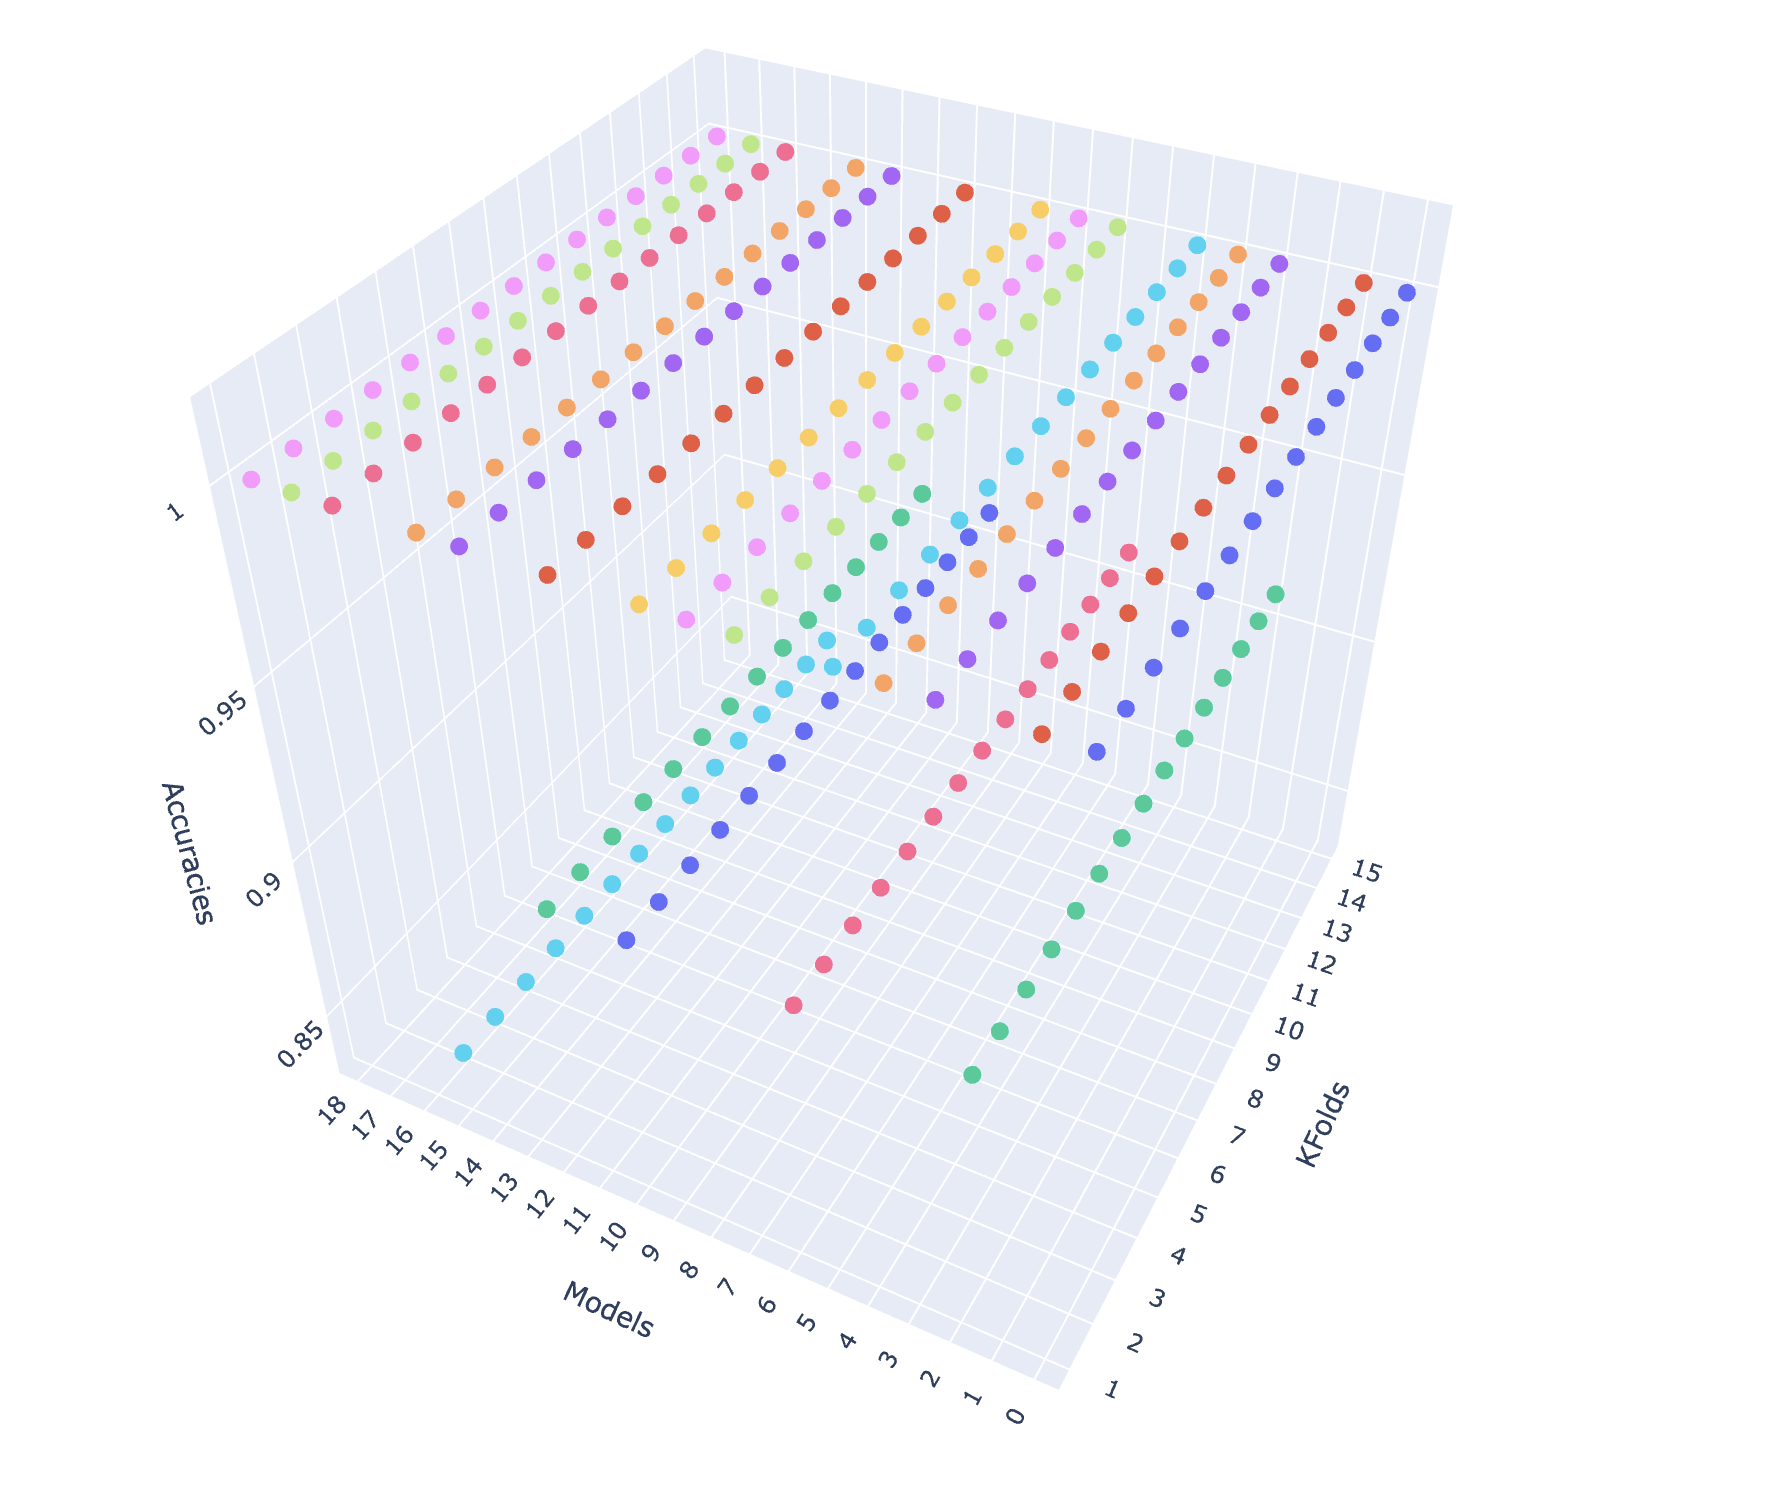
\includegraphics[height=9.2cm, width=\linewidth]{figures/accuracy_chart2.png}
		\caption{Models Accuracy}
		\label{fig:4}
	\end{figure}
	
	As shown from \ref{fig:4}, all the models accuracy in the initial system-level phase with, Wine Data from Table \ref{tab:Datasets}, were identical, and even by adding different noise types and values, the accuracy remained the same. These findings suggest that the QSVM operates as a deterministic rather than a stochastic system, or alternatively, that the noise implementation in PennyLane (v0.41) lacks true stochasticity. To implement noise in this version, the device configuration must be transitioned from lightning.qubit to default.mixed, as illustrated in Figure \ref{fig:5}. While physical IBM quantum hardware can be accessed via the qiskit.remote device type (see Figure \ref{fig:5}), this approach was not pursued due to the constraints detailed in Section \ref{sec:challenges_solutions}.
	
	\begin{figure}[H]
		\centering
		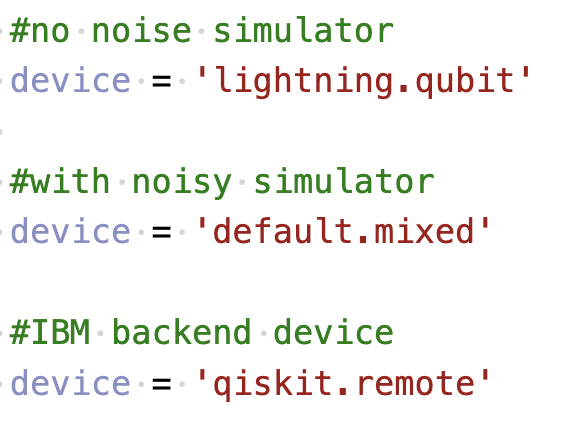
\includegraphics[height=2.3cm, width=\linewidth/2]{figures/devices.png}
		\caption{Pennylane Devices}
		\label{fig:5}
	\end{figure}
	
	
	Our subsequent evaluations revealed that introducing a specific number of shots to local simulators effectively injects randomness into the system, serving as an alternative to using a dedicated noisy device in Figure \ref{fig:6}, we show how the mutations are implemented in QSVM program. We are using intermediate managers to switch between mutated classes according to the mutation number provided. For example, if we are testing mutation \#1, then the feature map used will be from the \#1 mutated class of feature map class. All the mutants details can be found in Figures \ref{fig:11} through \ref{fig:18} in Appendix \ref{app:QSVMMutationsTable}.
	
	\begin{figure}[H]
		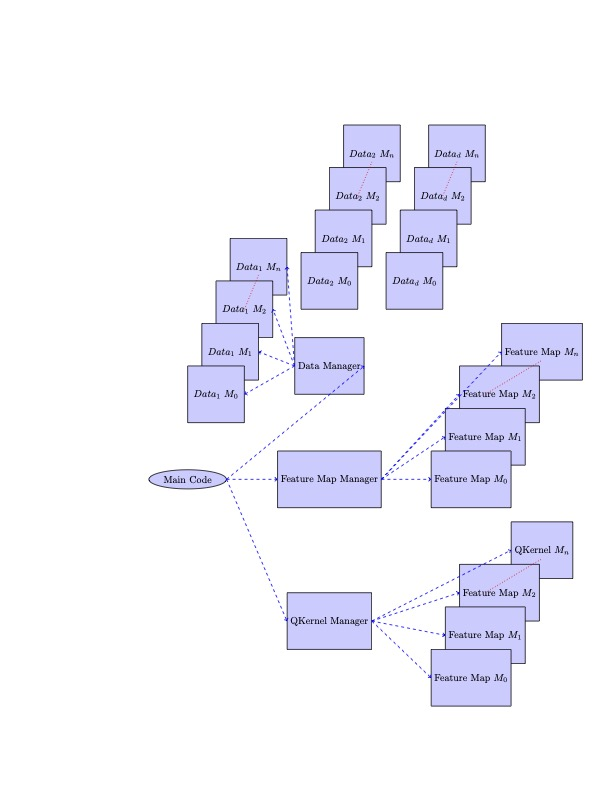
\includegraphics[height=15.2cm, width=\linewidth]{figures/Mutants_Classes.png}
		\caption{Mutations Implementation}
		\label{fig:6}
	\end{figure}
	
	\begin{figure}[H]
		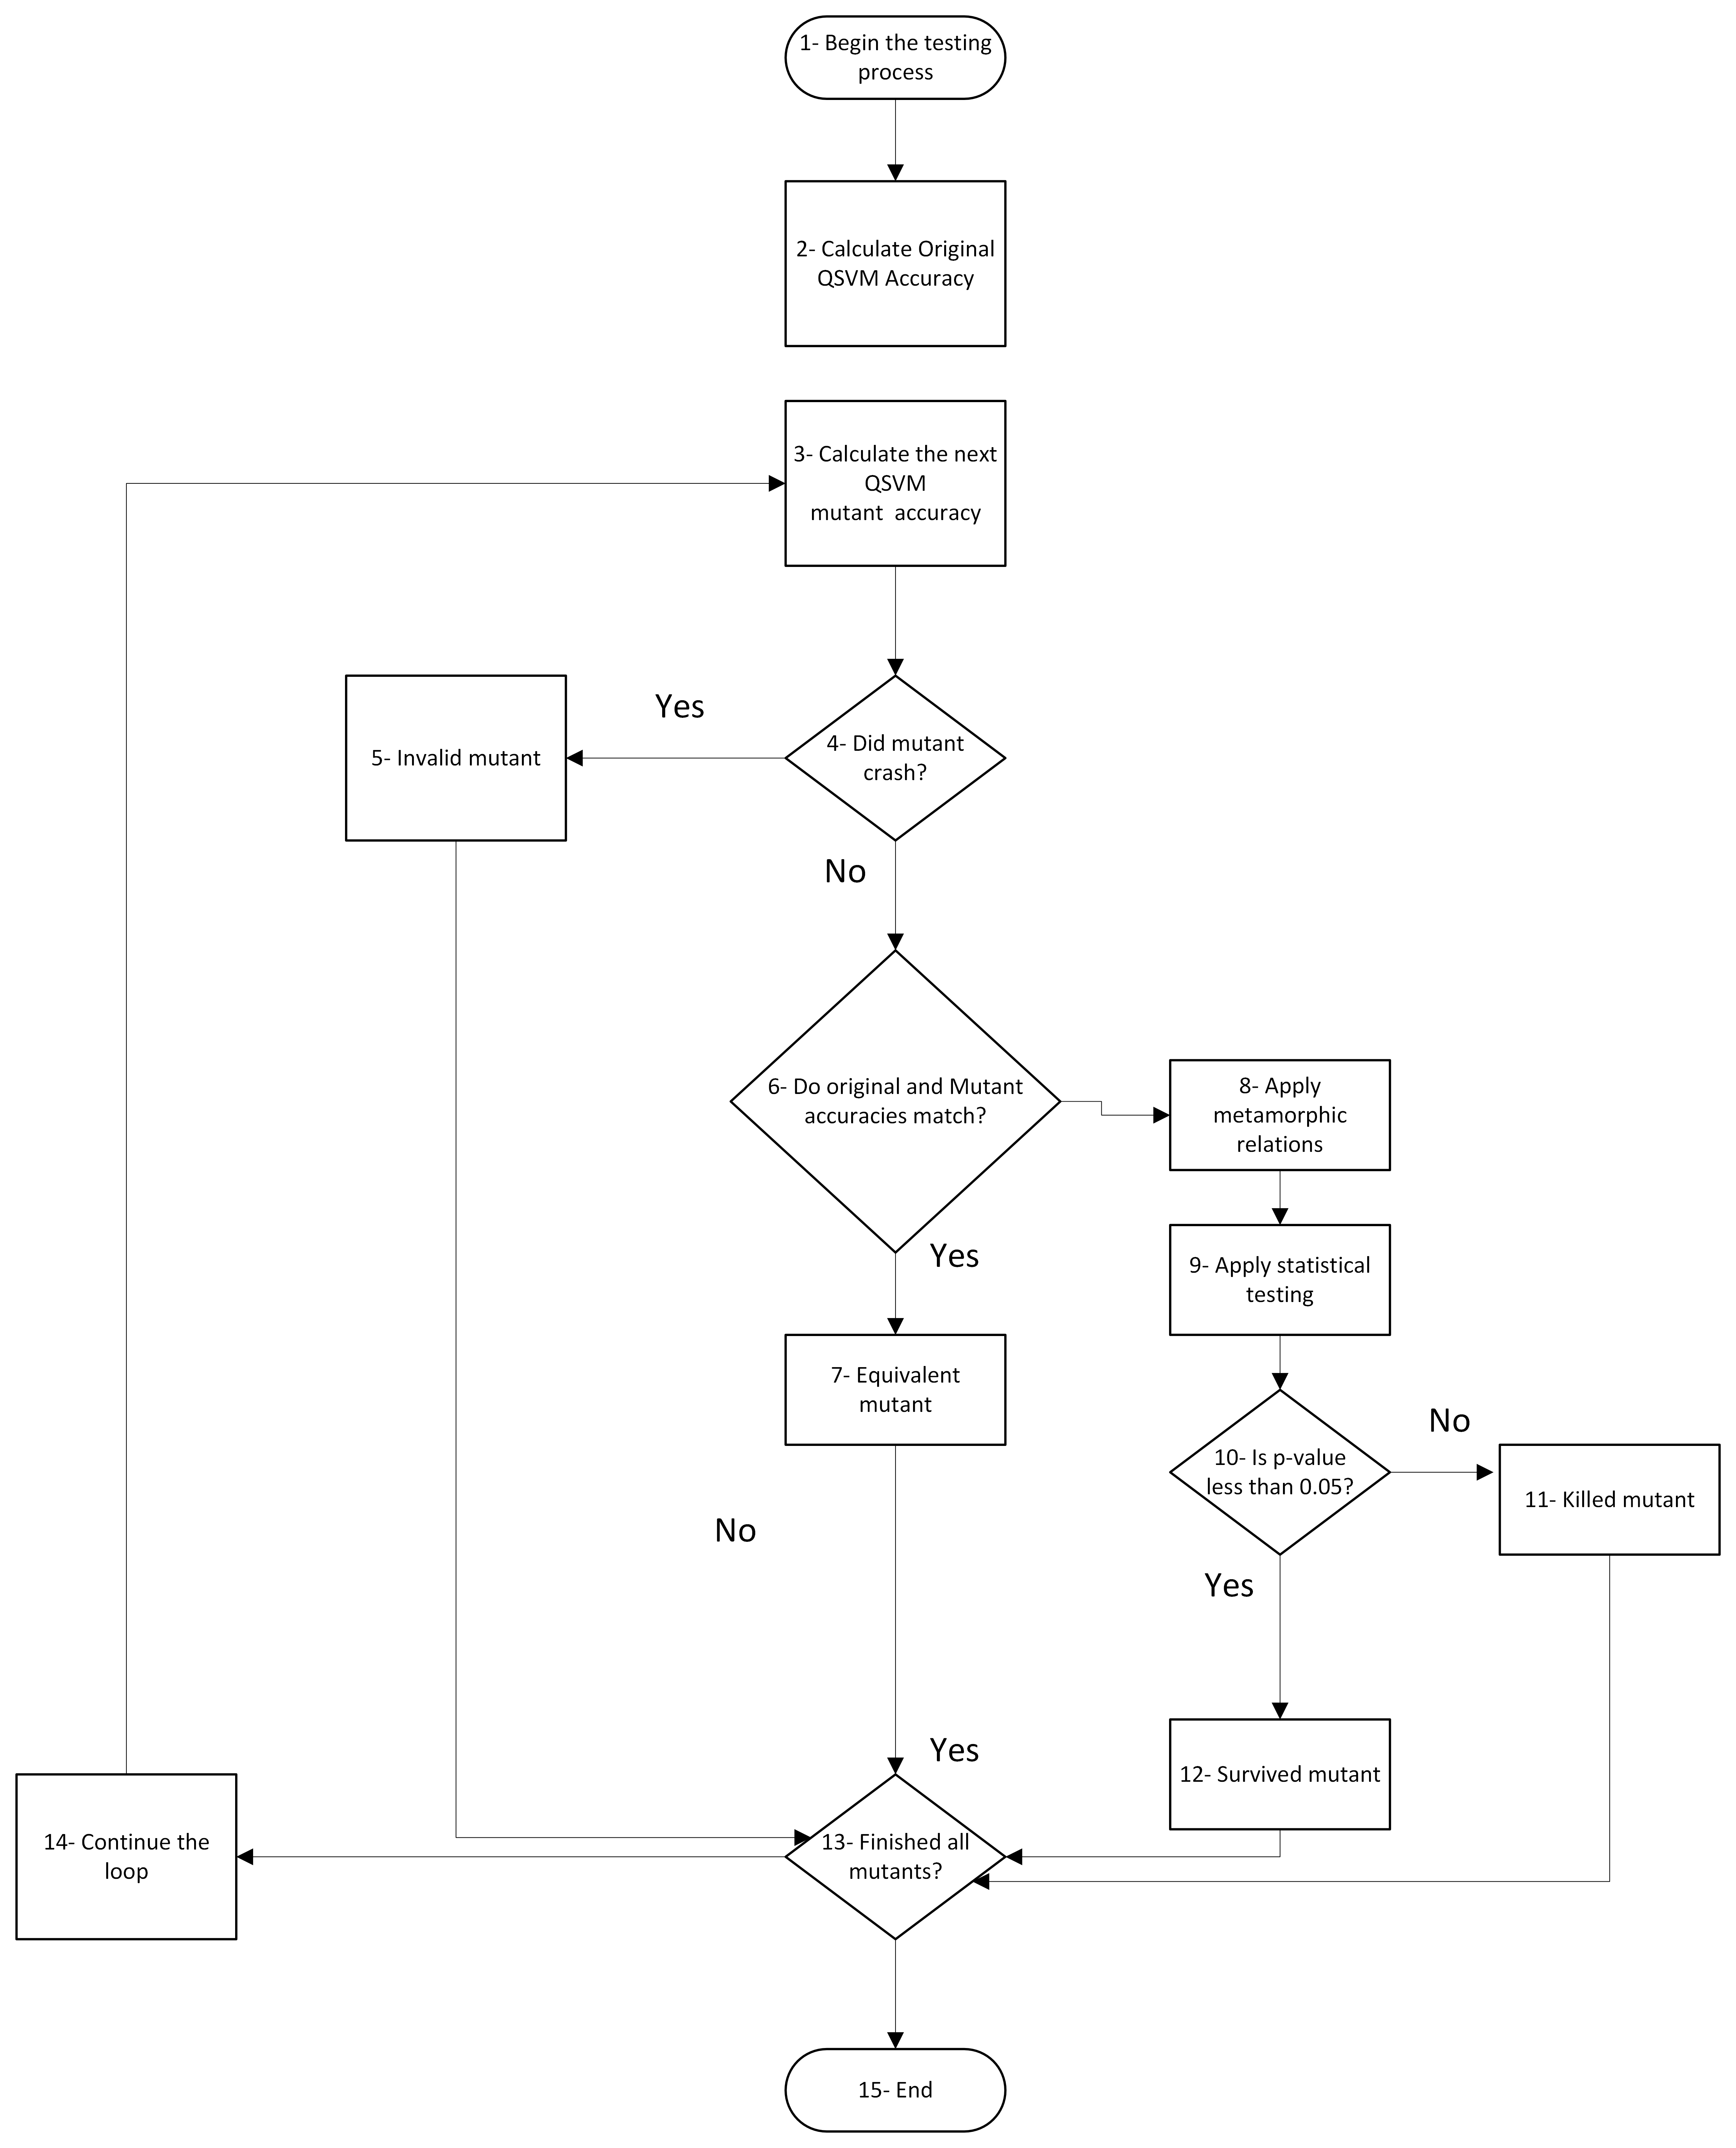
\includegraphics[height=15.2cm, width=\linewidth]{figures/QSVM_flowchart.png}
		\caption{Flowchart of testing QSVM}
		\label{fig:7}
	\end{figure}
	
	The final results for the system-level pipeline testing are shown in Figure \ref{fig:8}. MR\#1 killed the mutant \#1 and mutant \#26. MR\#2 killed mutant MR\#26, and MR\#3 killed mutant \#34. In Figure \ref{fig:9}, we can find that 10\% of the mutants were killed.
	
	\begin{figure}[H]
		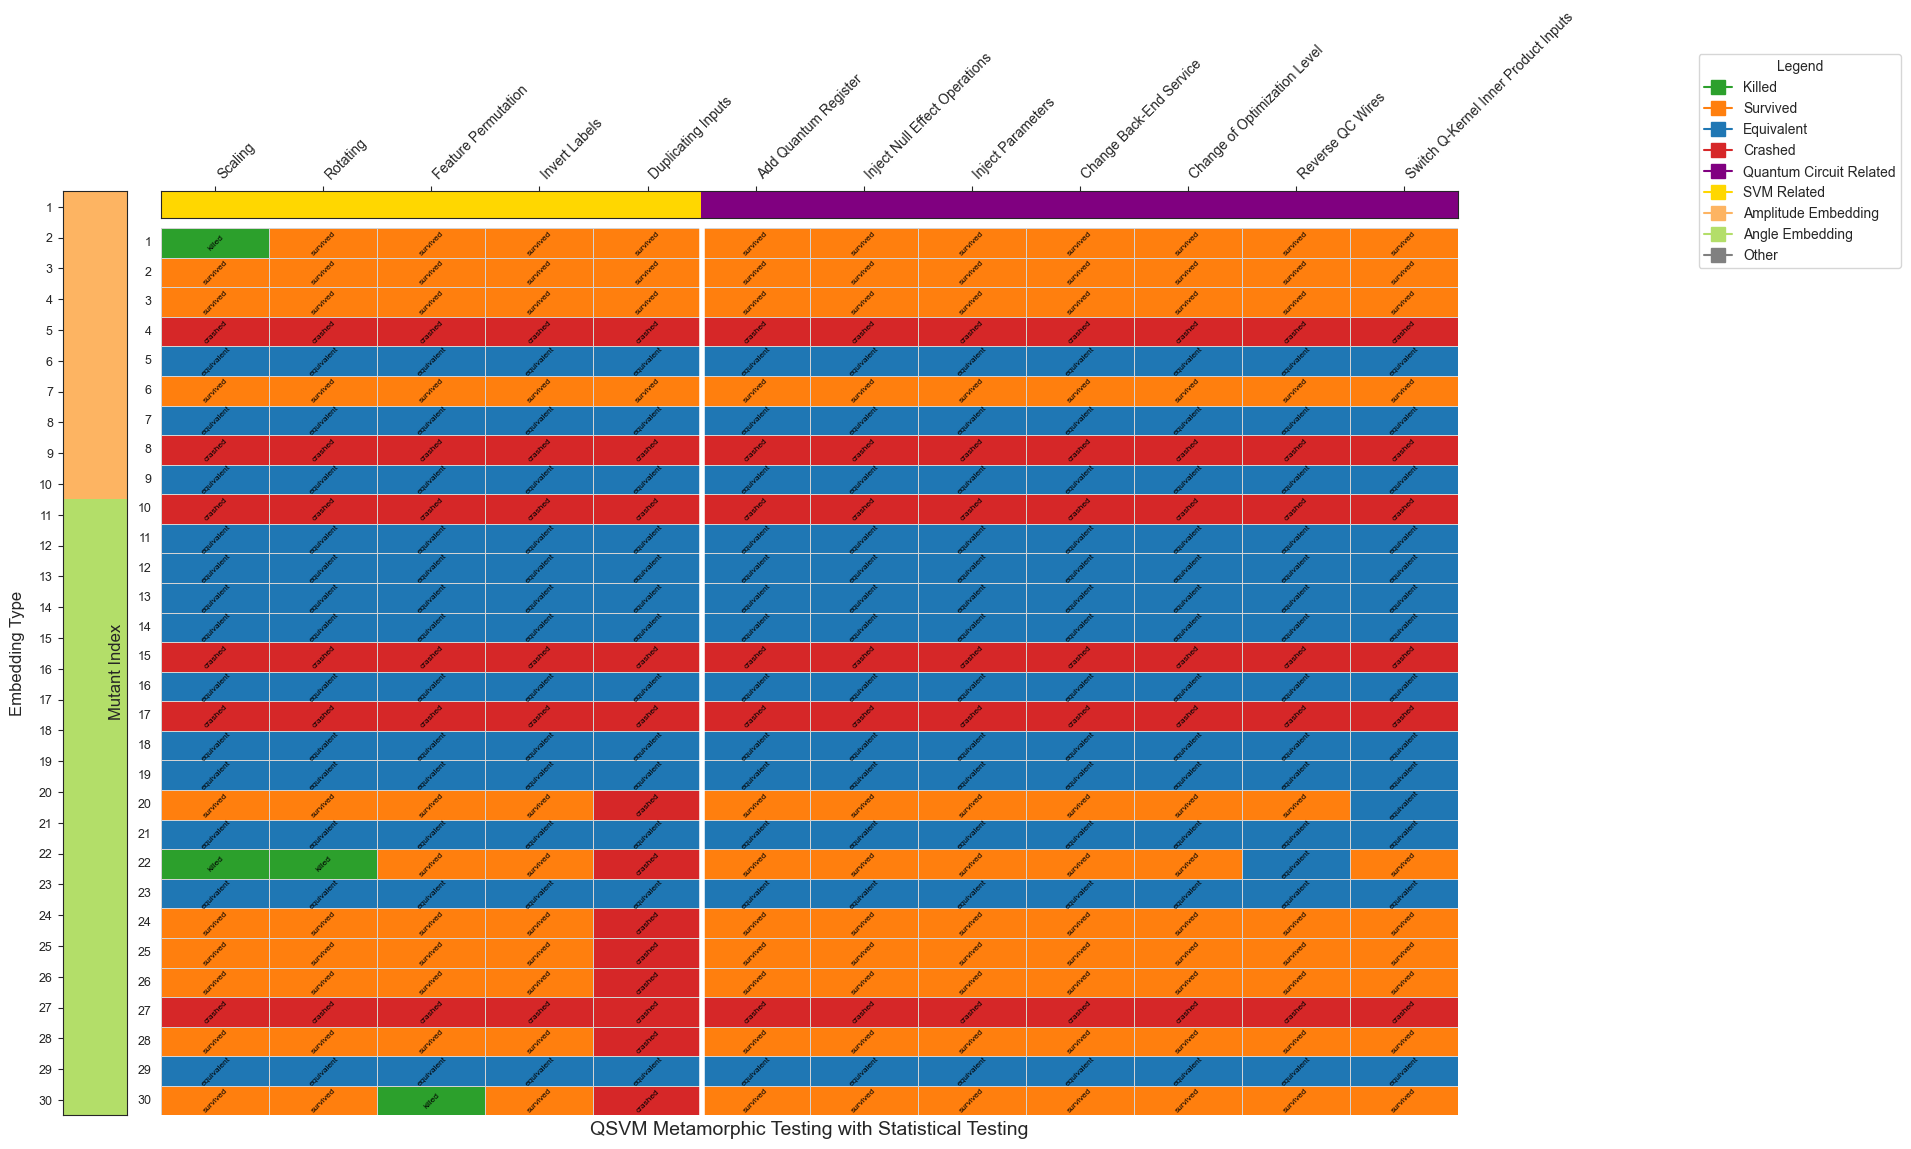
\includegraphics[height=18.2cm, width=\linewidth]{figures/mutant_outcome_fully_hierarchical_heatmap_sequential_labels_fixed_data.png}
		\caption{QSVM Testing Results}
		\label{fig:8}
	\end{figure}
	
	\begin{figure}[H]
		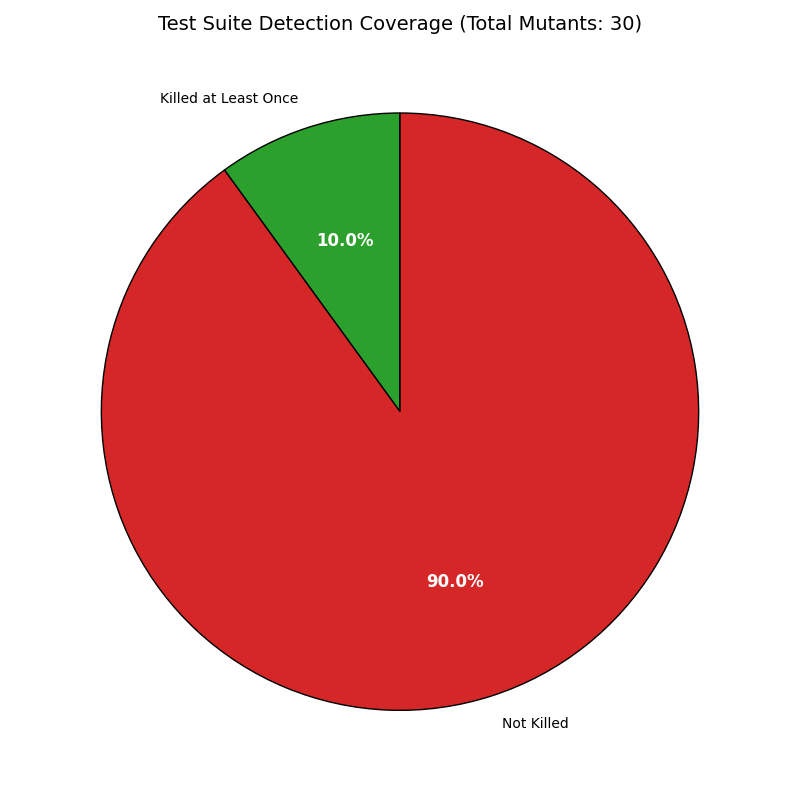
\includegraphics[height=15.2cm, width=\linewidth]{figures/mutant_detection_coverage_pie_chart.png}
		\caption{Killed Mutants Percentage}
		\label{fig:9}
	\end{figure}
	
	When we tested in the beginning with the scaling MR for SVM and the angle rotation MR, the metamorphic testing score was equal to 0, from Equation \ref{eq:MTS}. This shows that there is no difference between all the models regardless of the modifications, and this means there is not any stochastic factor when using QSVM in Qiskit and Pennylane. And in the subsequent phases,  and then mutation operators were added to add bugs to QSVM program, to measure the metamorphic relations more effectively \cite{9678563}. 
	
	To address the low kill rate of system-level relations, the targeted quantum kernel experiment was conducted with 100 runs since the mutator is non-deterministic, and to provide statistical results. In Figure \ref{fig:v41_confidence}, we can see that 96\% of the mutants were killed in general in amplitude embedding, angle embedding and basis embedding.
	
	The heatmap analysis, from Figure \ref{fig:v41_heatmap}, reveals that \textbf{MR2 (Identity)} is the "Universal Oracle," catching nearly all structural and logic defects across all modes, and comes after it \textbf{MR12} and \textbf{MR1} equivalently.
	
	\begin{itemize}
		\item \textbf{Basis Embedding}: Most of the mutants were killed by  MR2 and then followed by  MR10
		\item \textbf{Angle Embedding}: Most of the mutants were killed by MR1, MR2, MR3, MR4, and MR7 equally and some by MR12 then followed by MR5
		\item \textbf{Amplitude Embedding}: MR1 and MR2 killed the majority of mutants, and some by MR9, then followed by MR11 and MR3 equally
	\end{itemize}
	
	\begin{figure}[H]
		\centering
		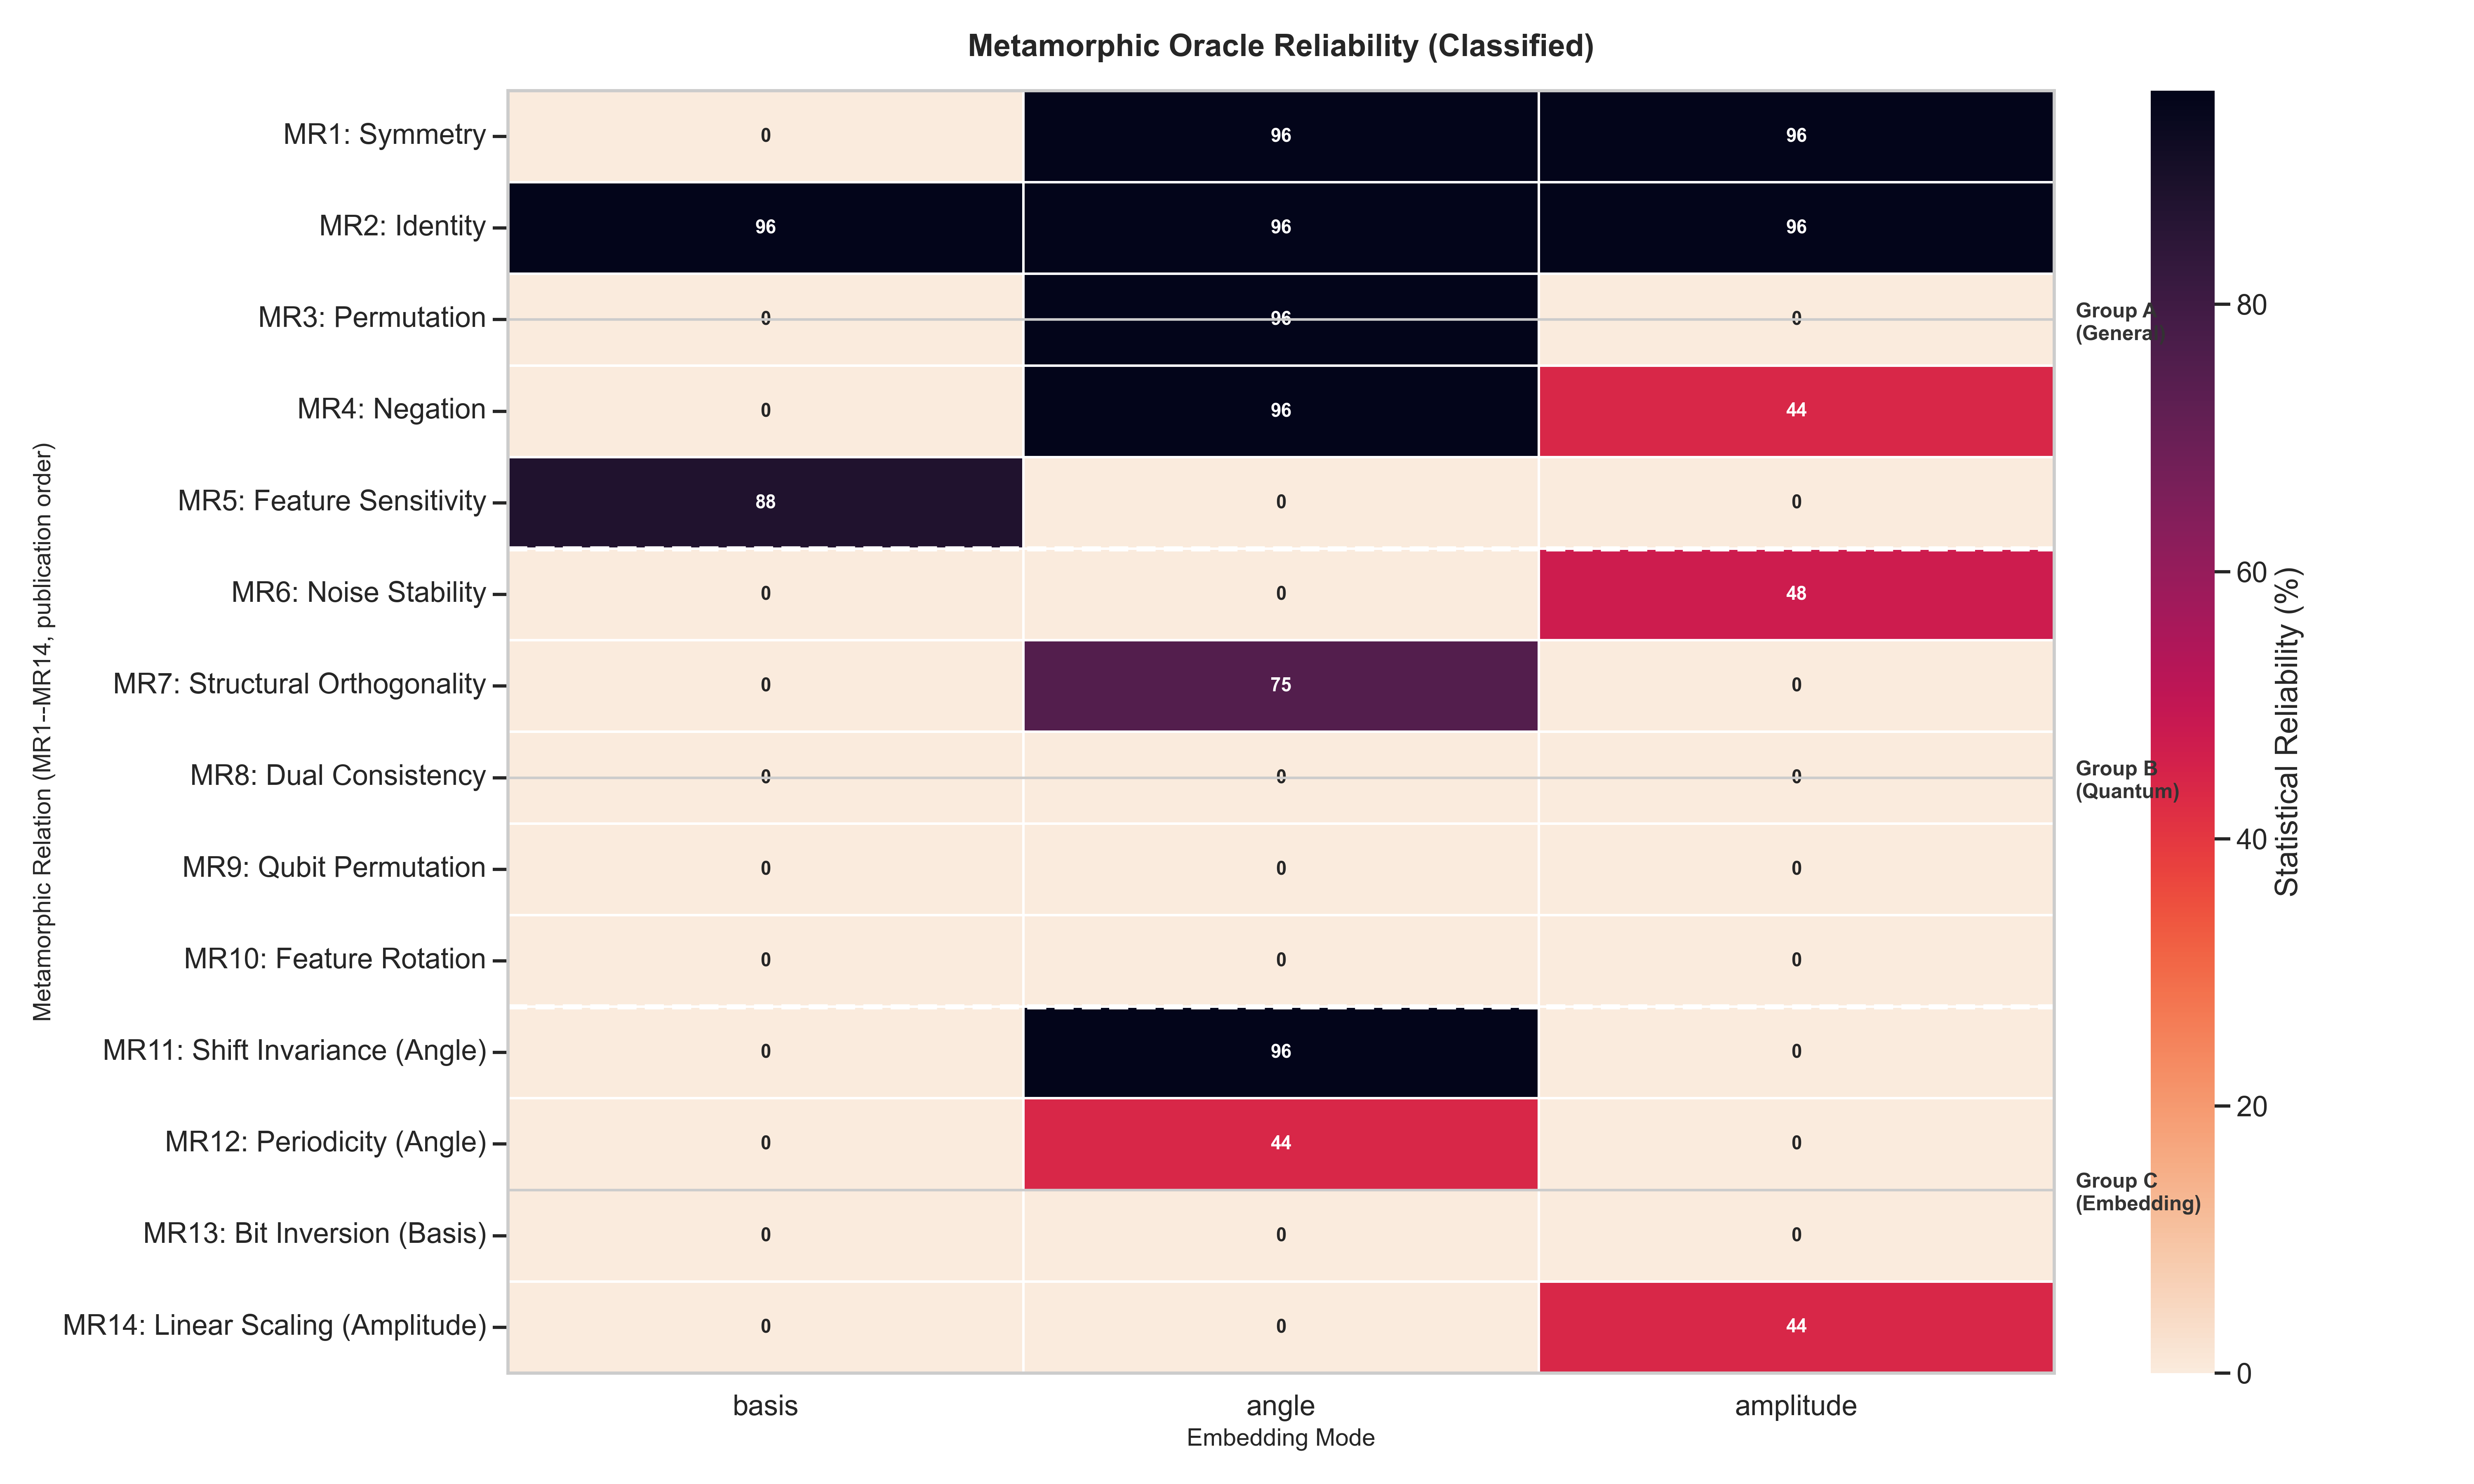
\includegraphics[width=1.0\textwidth]{figures2/chart_v41_heatmap_omni_2.png}
		\caption{Omni-Suite Heatmap: Comparing the statistical reliability of all 14 MRs.}
		\label{fig:v41_heatmap}
	\end{figure}
	
	\begin{figure}[H]
		\centering
		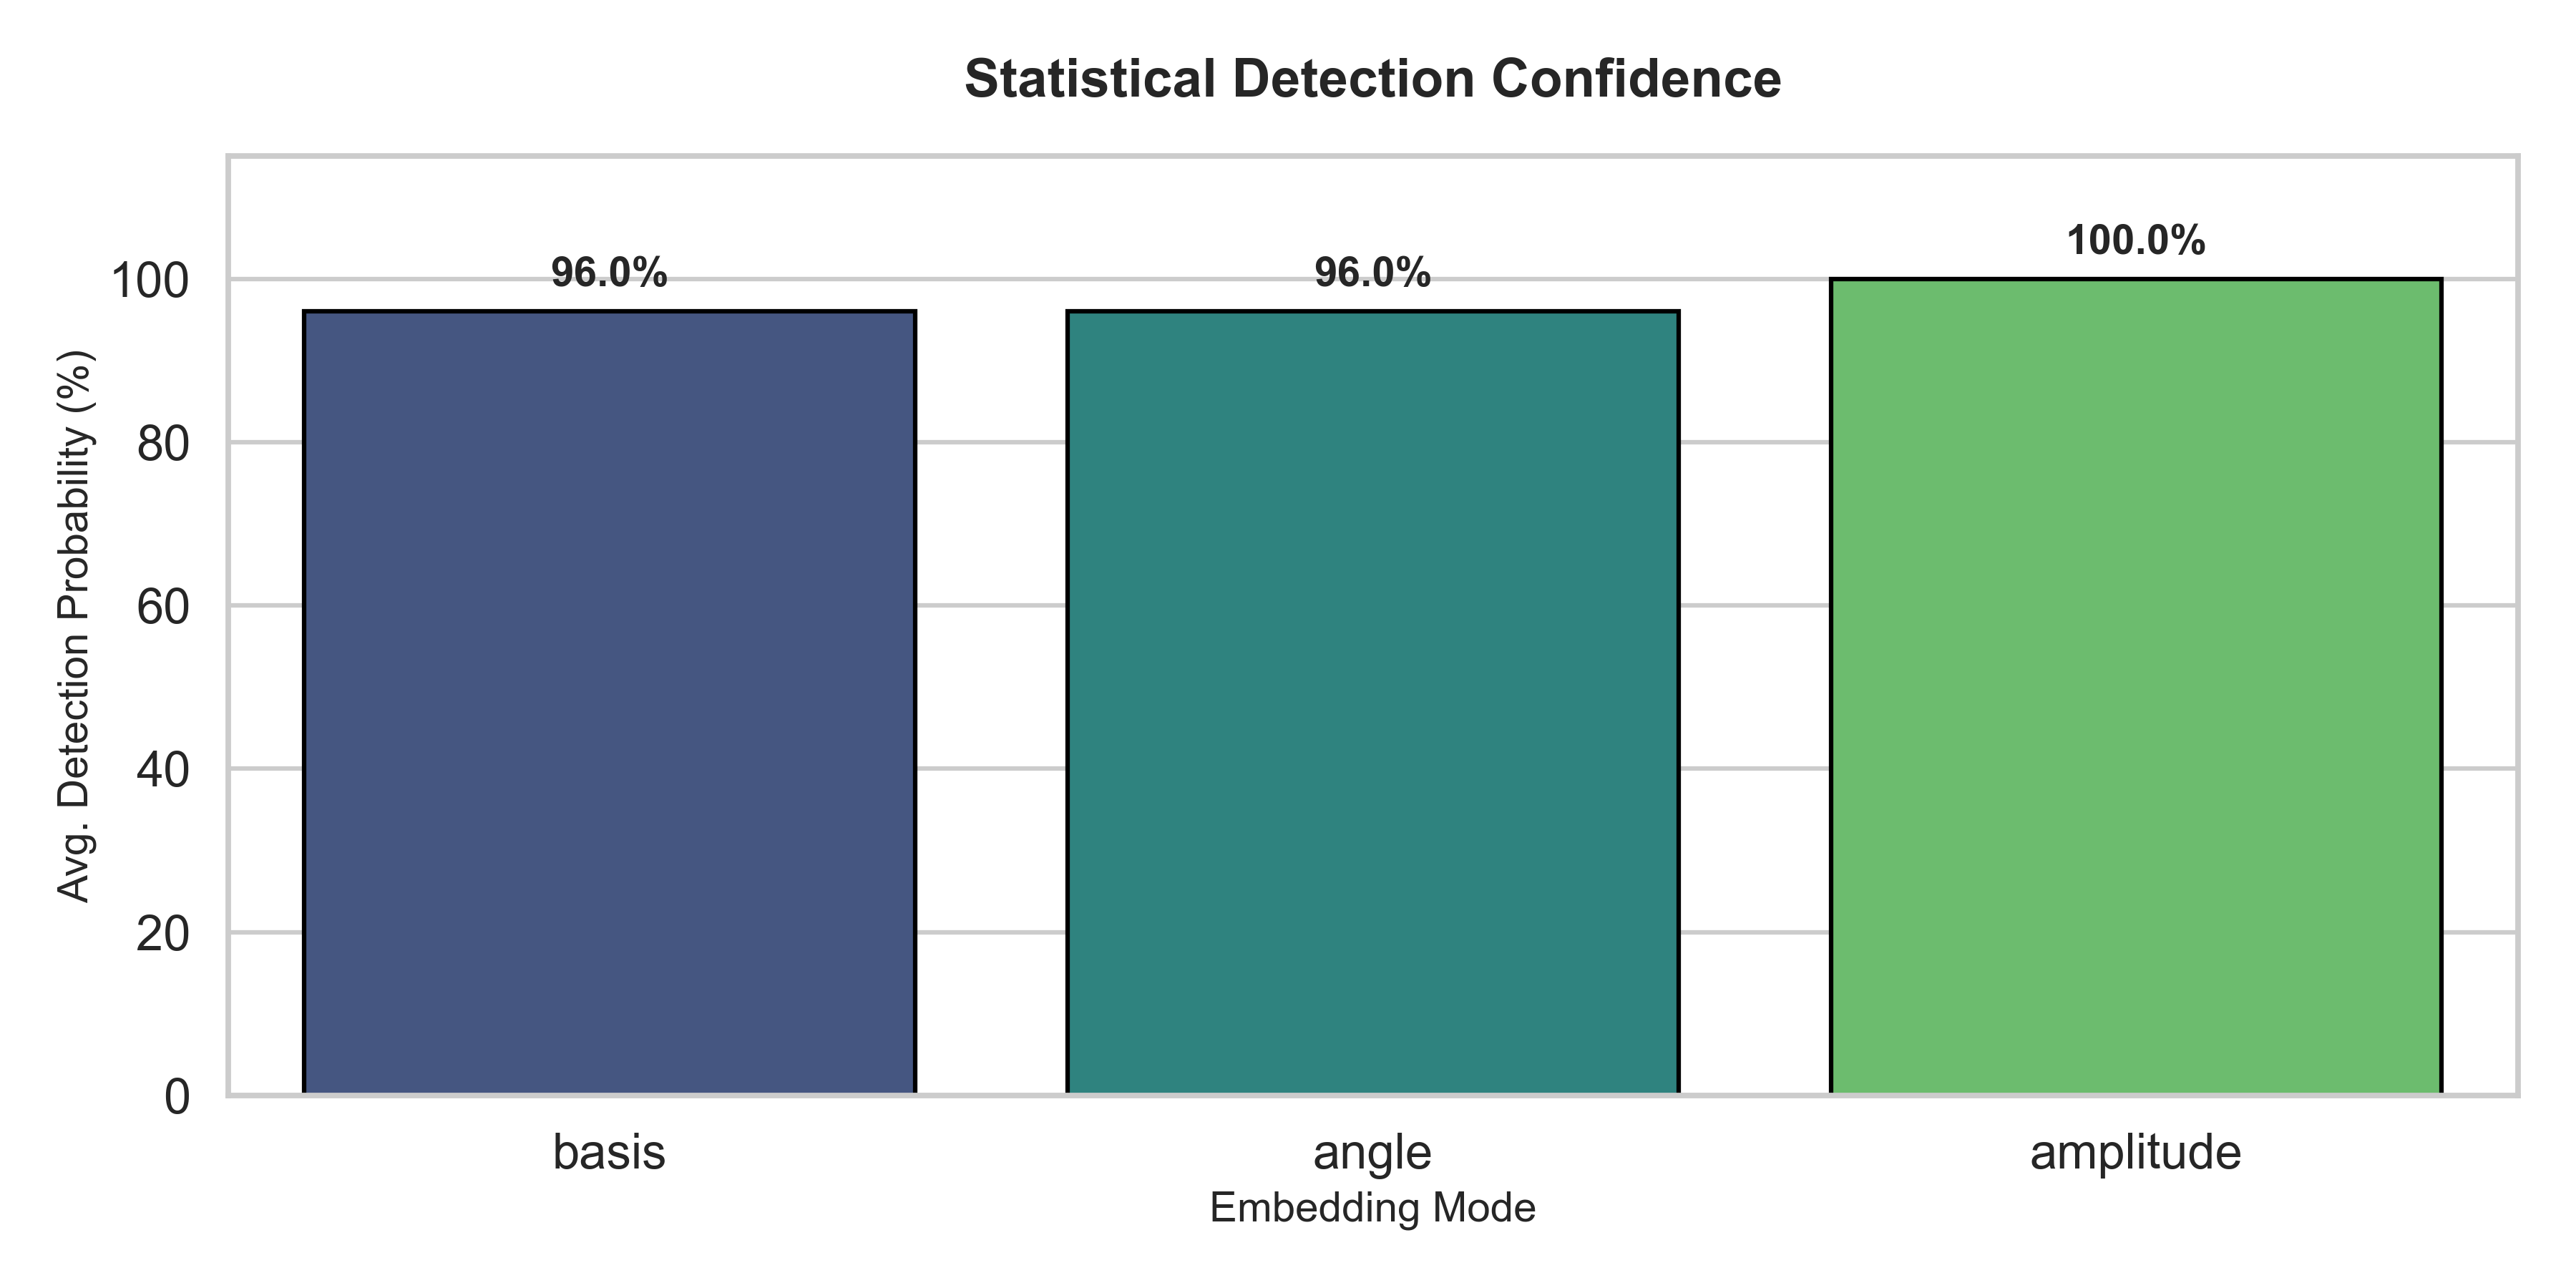
\includegraphics[width=1.0\textwidth]{figures2/chart_v41_detection_omni_2.png}
		\caption{Detection Confidence: High robustness achieved across all encoding schemes.}
		\label{fig:v41_confidence}
	\end{figure}
	
	For the research questions (RQs) in this section, the answers are still under progress but here are our findings. for RQ1, MR\#1 was the most efficient system-level MRs because it killed two mutants. At the kernel level, MR2 was the most effective. Then, we have MR\#1 and MR\#3 as the second most effective since both of them. For RQ2, it seems we need to find more effective metamorphic relations since the system-level ones only killed 10\% of bugs. Also, another possible way to modify the test to apply different metamorphic relations for each component of QSVM like feature map independently. For RQ3, even though it was concluded that the QSVM is not stochastic, we could still benefit from statistical testing to kill mutants. We might need to connect to a back-end device to work with real noisy devices to analyze if the MRs can cope up with noise if desired. Finally, for RQ4, the answer is that by testing the quantum kernel, we managed kill 96\% of the mutants created that showed drastic changes in the quantum kernel functionality, in all feature maps.
	
	\subsection{Reflections, Challenges, and Solutions}
	\label{sec:challenges_solutions}
	
	
	One of the major challenges we faced in our experiments is that Qiskit related libraries versions need to be manually adjusted to be compatible with each other. Another challenge is that Pennylane abstracts the code and does not allow for a lot of customization as in Qiskit. Moreover, Pennylane's latest version as of this report is below 1.0 which shows that it is still in an experimental phase. Finally, training QSVM models takes a lot of time especially if we add noise. And it also depends on the number of inputs, the data dimension and how many k-folds are used, the training time for all models can take from a couple of hours to a couple of days. The last challenge is to have a comprehensive automated tool to create mutants, since the mutants used in our initial system-level metamorphic testing were manually modified.
	
	To solve the compatibility problem with Pennylane and Qiskit along with the randomness issue in Pennylane noise, the code can be fully re-implemented with Qiskit code only or even try another library like Qiskit-Machine-Learning. Moreover, the lengthy training time when implementing noise can be resolved by relying on using IBM back-end service as a real quantum computer instead of the simulation. However, the free tier offered by IBM provided only 10 minutes to run tests. In future, we can aim to expand our tests on IBM back-end services.
	
	To address the limitations of manual mutant generation, we implemented the dynamic AutoMutator for the kernel-level metamorphic testing, where the mutation tool was specifically targeting the three feature maps and quantum kernel we used.. Instead of testing QSVM as a comprehensive pipeline, we focused on testing the quantum component, addressing the abstract feature maps in Pennylane by making the code more expressive and explicit.
	
	But still, the mutants used in the system-level testing phase were created manually, which alludes to them not being exhaustive of all different variations. The experiment can be repeated with an automation tool to create mutants or can be repeated on more different mutants created manually.
	
	We would like to mention that more metamorphic relations can be used in testing QSVM to improve the test results presented in this Section. However, finding metamorphic relations takes a lot of time, and it took a lot of time to accumulate the necessary knowledge around software testing, machine learning, and quantum computer for this report. However, in future we can work on improving the results in this report.
	
	\section{Conclusion and Next Plan}
	\label{sec:conclusion}
	
	\subsection{Conclusion}
	
	On a high level, QSVM is still more of a machine learning algorithm rather than a quantum algorithm. Subsequently, testing QSVM as a whole pipeline with different metamorphic relations showed that the metamorphic relations related to SVM were more effective than the ones related to Quantum Computing. However, the possibility stands that there could be more effective metamorphic relations that could be used and could be more effective. But, finding these metamorphic relations will need more work and research. 
	
	In the last experiment, when we tested only the quantum element in QSVM, and we managed to kill almost all the mutants using 14 quantum kernel metamorphic relations with a success rate of 96\%. The kernel-level testing phase were generally more promising than the level-testing phase.
		
	\subsection{Work Plan for Next Period}
	\label{sec:next-plan}
	
	One of the plans is to use Qiskit directly for QML e.g., QSVM, or another tool besides Pennylane. We found another tool named Qiskit Machine Learning and the latest version is 0.9.0 as of Dec 2025. We might need to re-implement some parts of the code and run these experiments again.  Also, we can move from QSVM to a convolutional neural networks algorithm to use a stochastic system instead of QSVM. Moreover, for mutation testing, we can work on creating a more comprehensive automated tool to add modifications to the program to intentionally introduce some bugs in the system under test (SUT) \cite{qMutphyFortunato}. Besides that, we can research more effective metamorphic relations to detect more mutants and kill them. For the last phase of kernel-level testing, we can incorporate statistical testing in a bigger test short term. In long term, we will move afterwards to testing Quantum Convolutional Neural Networks (QCNNs). 
	
	\subsection{study plan}
	
	The Gantt Chart for study plan is shown in the appendix (see Figure \ref{fig:10}). The first thing to do next is start working on Quantum Convolutional Neural Networks (QCNNs) after the upgrade. Then, Statistical testing will be applied on QCNNs along with mutation testing. 
	
	After that, in the third year advanced testing techniques can be used. Then after that, the work to finalize the dissertation will start.
	
	\begin{comment}
		\section{Supervisor's Comments (Optional)}
		\label{sec:supervisor-comments}
		This section can be left for your supervisor to add their comments if required by your institution.
	\end{comment}
	
	\begin{comment}
		\section{Concluding Remarks }
		\label{sec:conclusion}
		To be discussed ....
	\end{comment}
	
	
	\section*{Data and Code Availability}
	The source code used to generate the results and mutants in this report is publicly available on GitHub at \url{https://github.com/fox880919/qsvm-testing-structured}. Additionally, the executable files required for reproducing the experiments can be accessed via Google Drive at \url{https://drive.google.com/drive/folders/1ZgRW2NwCZaJVruJArUiF7Q_nKT4E3B52}.
	
	%\printbibliography % Prints your bibliography
	
	\bibliographystyle{IEEEtran}	
	\bibliography{references} % Your .bib file (without extension)
	
	\clearpage 
	
	\begin{appendices}
		
		\section{Gantt Chart}
		\begin{figure}[ht!]
			
\includegraphics[angle=90, height = 21.1 cm ,width=\linewidth]{figures2/study_plan.png}
			
			\caption{Study Plan}
			\label{fig:10}
		\end{figure}
		
		\section {QSVM Mutations Table}
		\label{app:QSVMMutationsTable}
		
		\begin{figure}[ht!]
			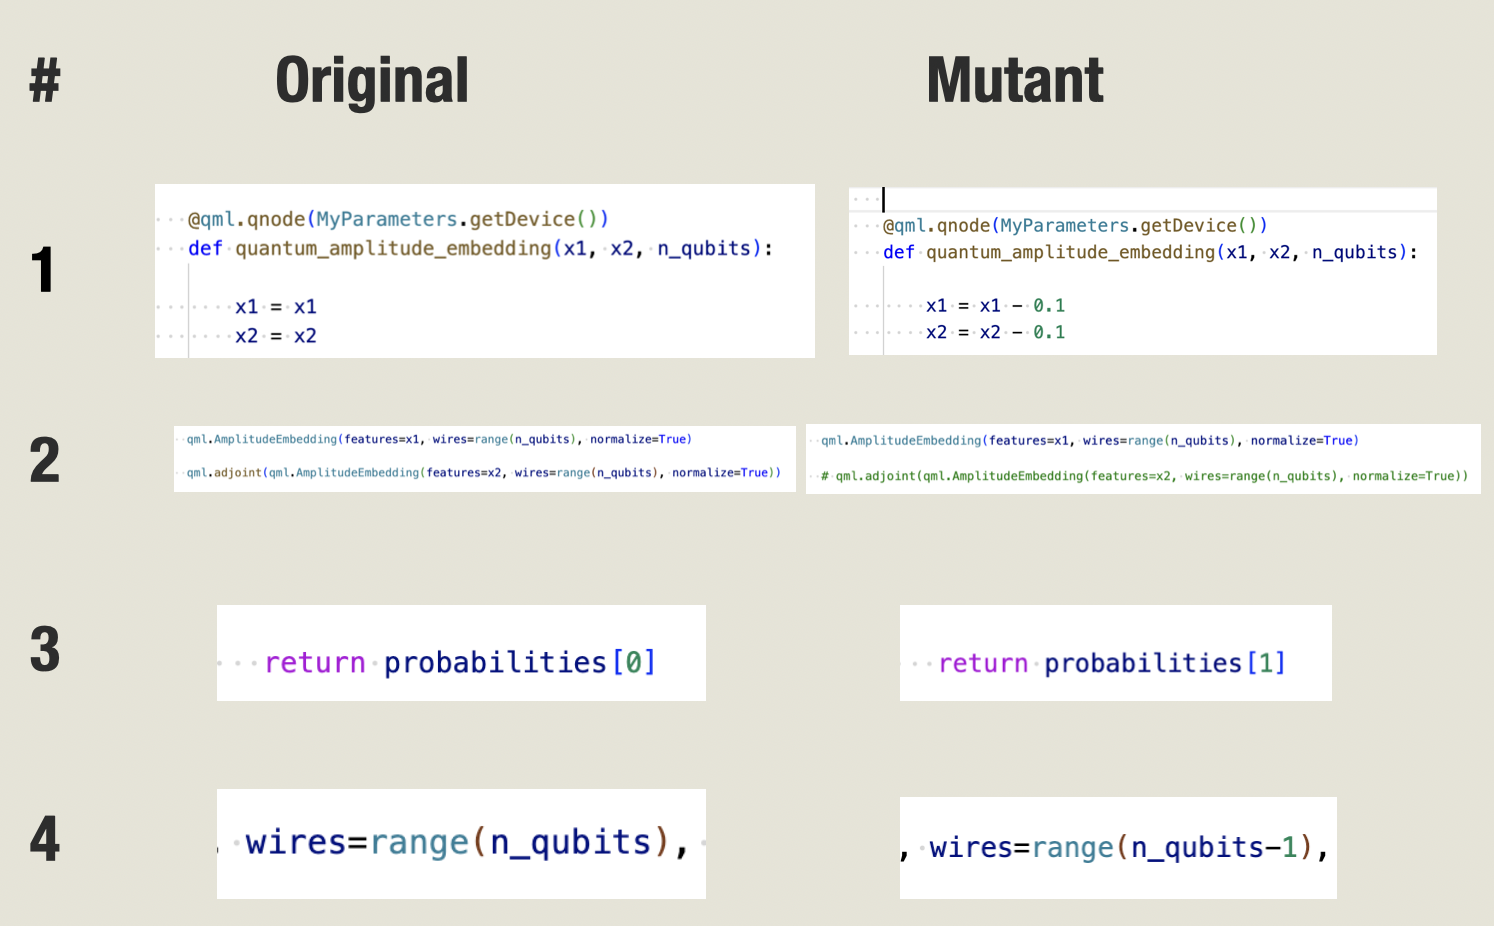
\includegraphics[height = 7 cm ,width=\linewidth]{figures/MT_1.png}
			\caption{QSVM Mutations Table \#1}
			\label{fig:11}
		\end{figure}
		
		\begin{figure}[ht!]
			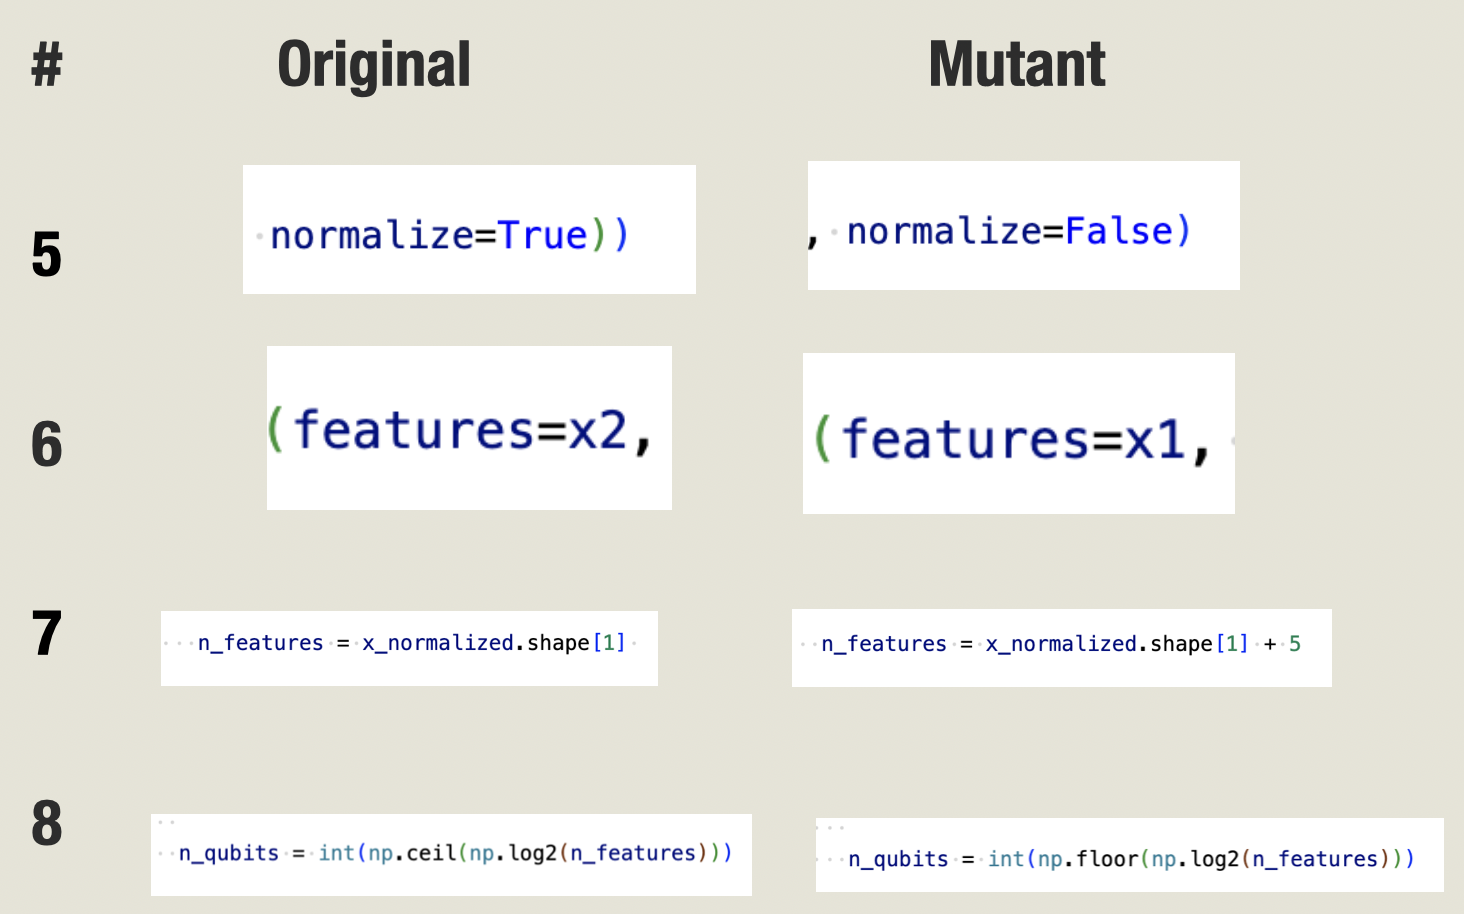
\includegraphics[height = 7 cm ,width=\linewidth]{figures/MT_2.png}
			\caption{QSVM Mutations Table \#2}
			\label{fig:12}
		\end{figure}
		
		\begin{figure}[ht!]
			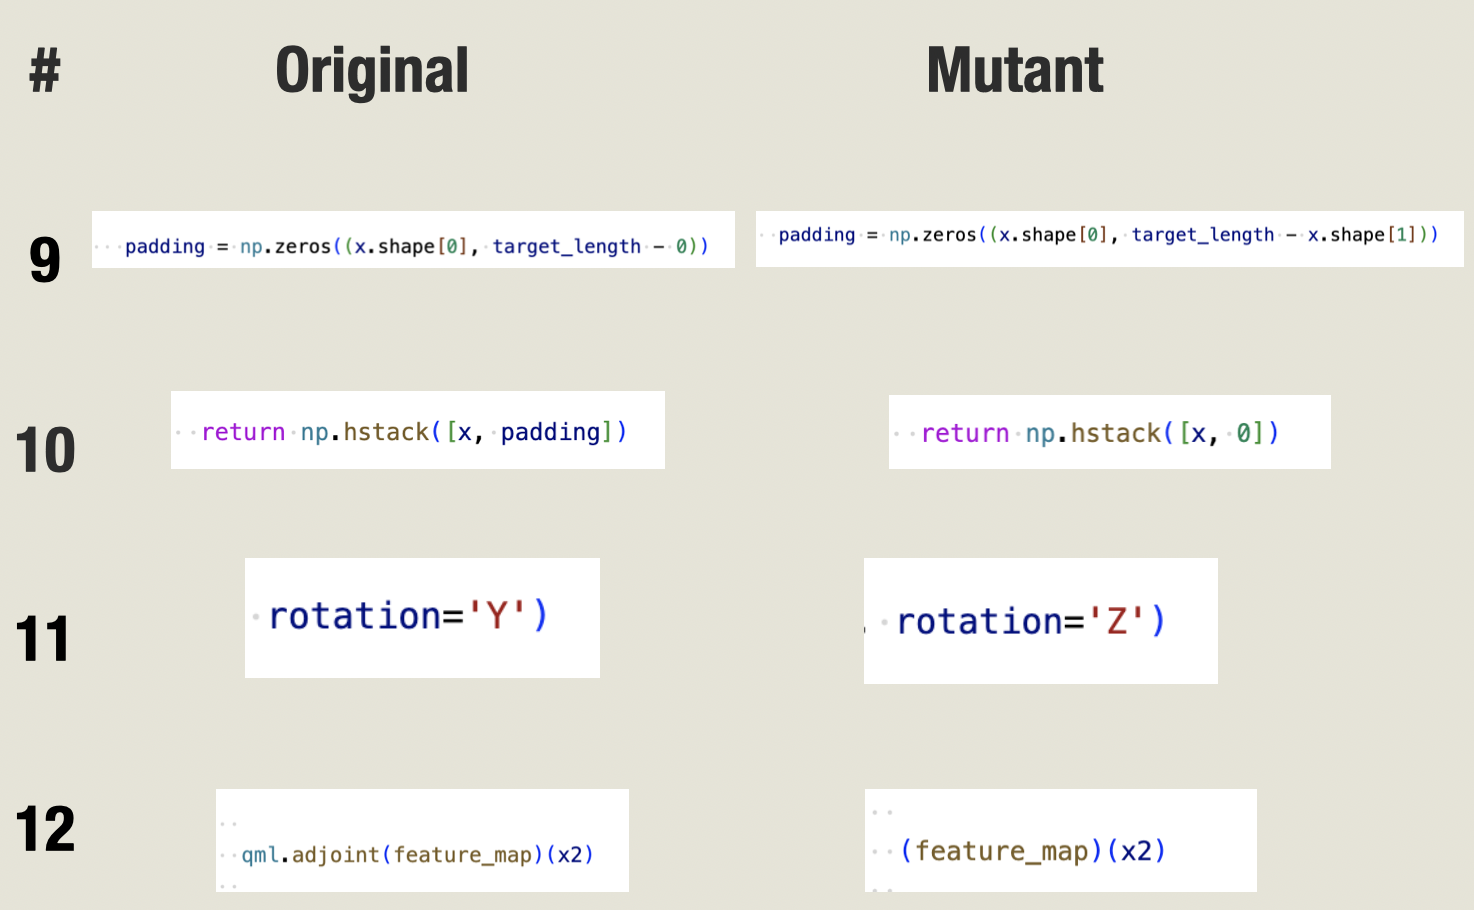
\includegraphics[height = 7 cm ,width=\linewidth]{figures/MT_3.png}
			\caption{QSVM Mutations Table \#3}
			\label{fig:13}
		\end{figure}
		
		\begin{figure}[ht!]
			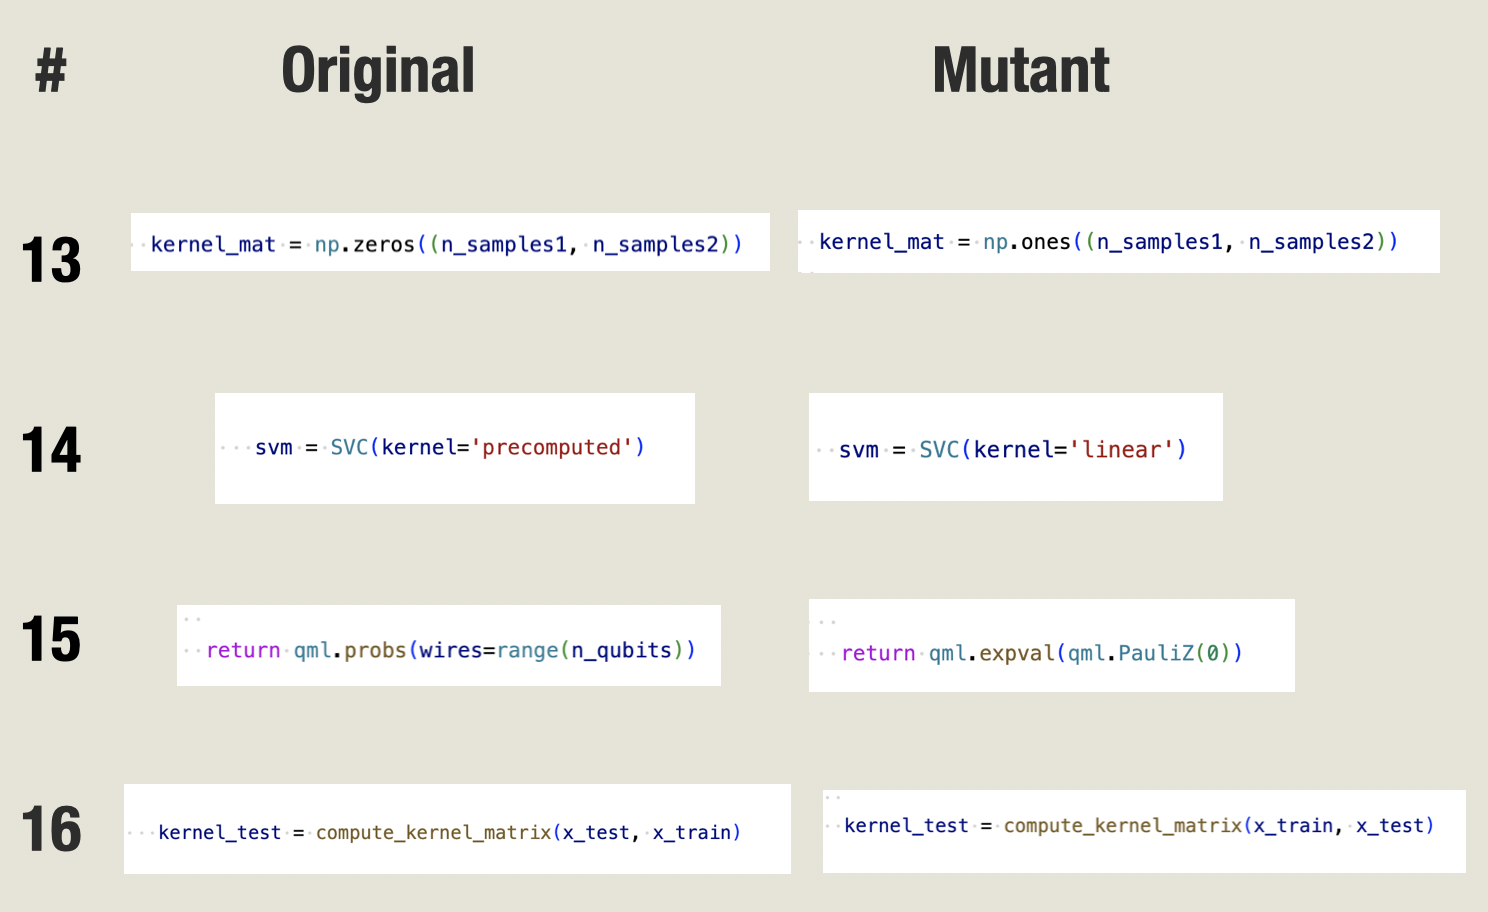
\includegraphics[height = 7 cm ,width=\linewidth]{figures/MT_4.png}
			\caption{QSVM Mutations Table \#4}
			\label{fig:14}
		\end{figure}
		
		\begin{figure}[ht!]
			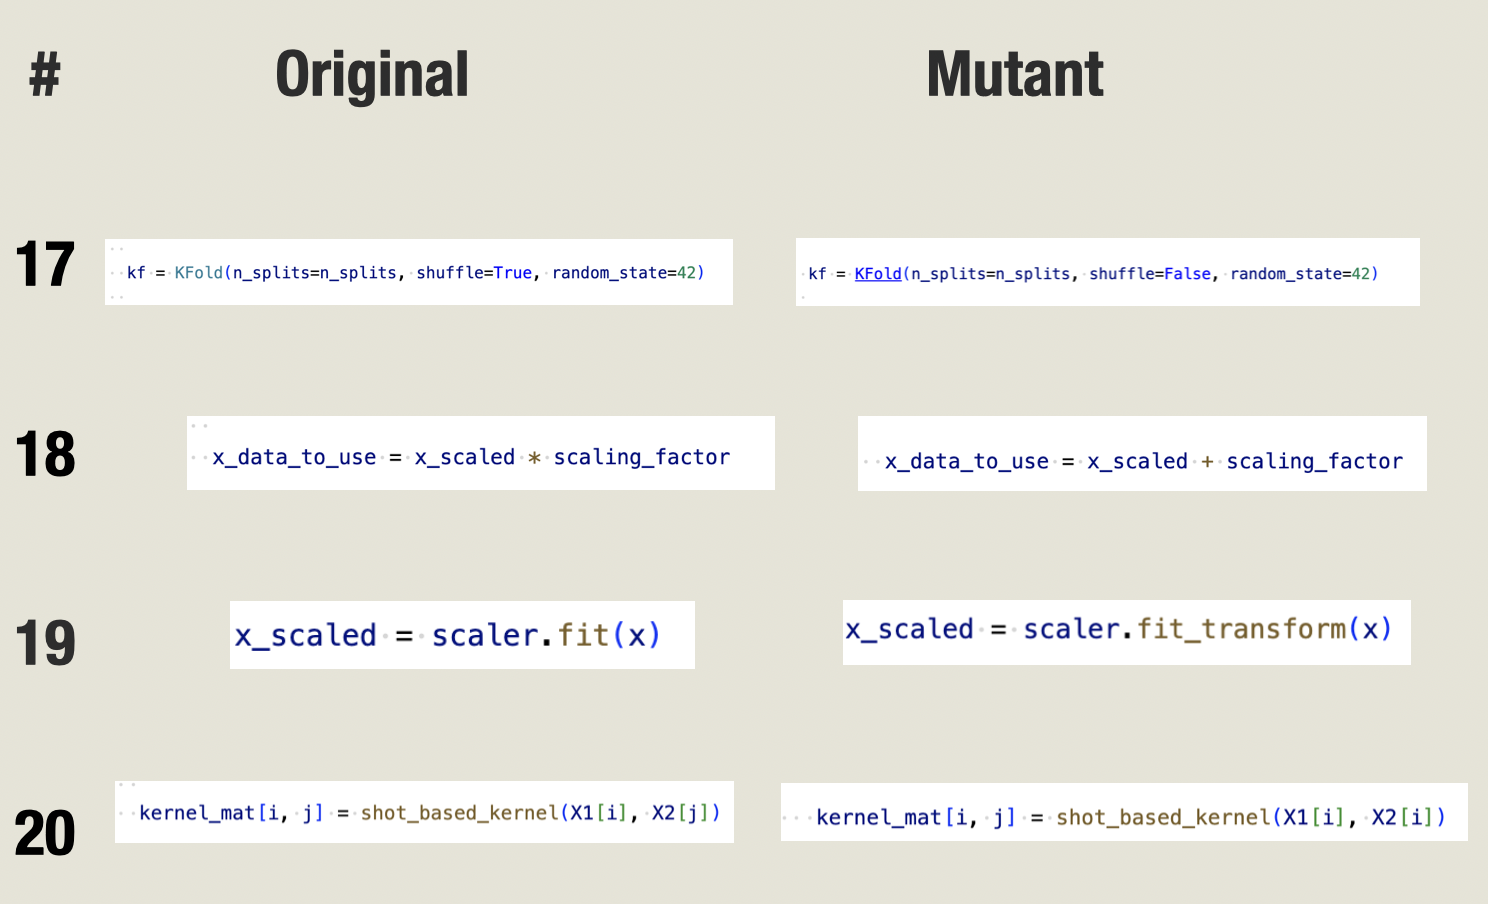
\includegraphics[height = 7 cm ,width=\linewidth]{figures/MT_5.png}
			\caption{QSVM Mutations Table \#5}
			\label{fig:15}
		\end{figure}
		
		\begin{figure}[ht!]
			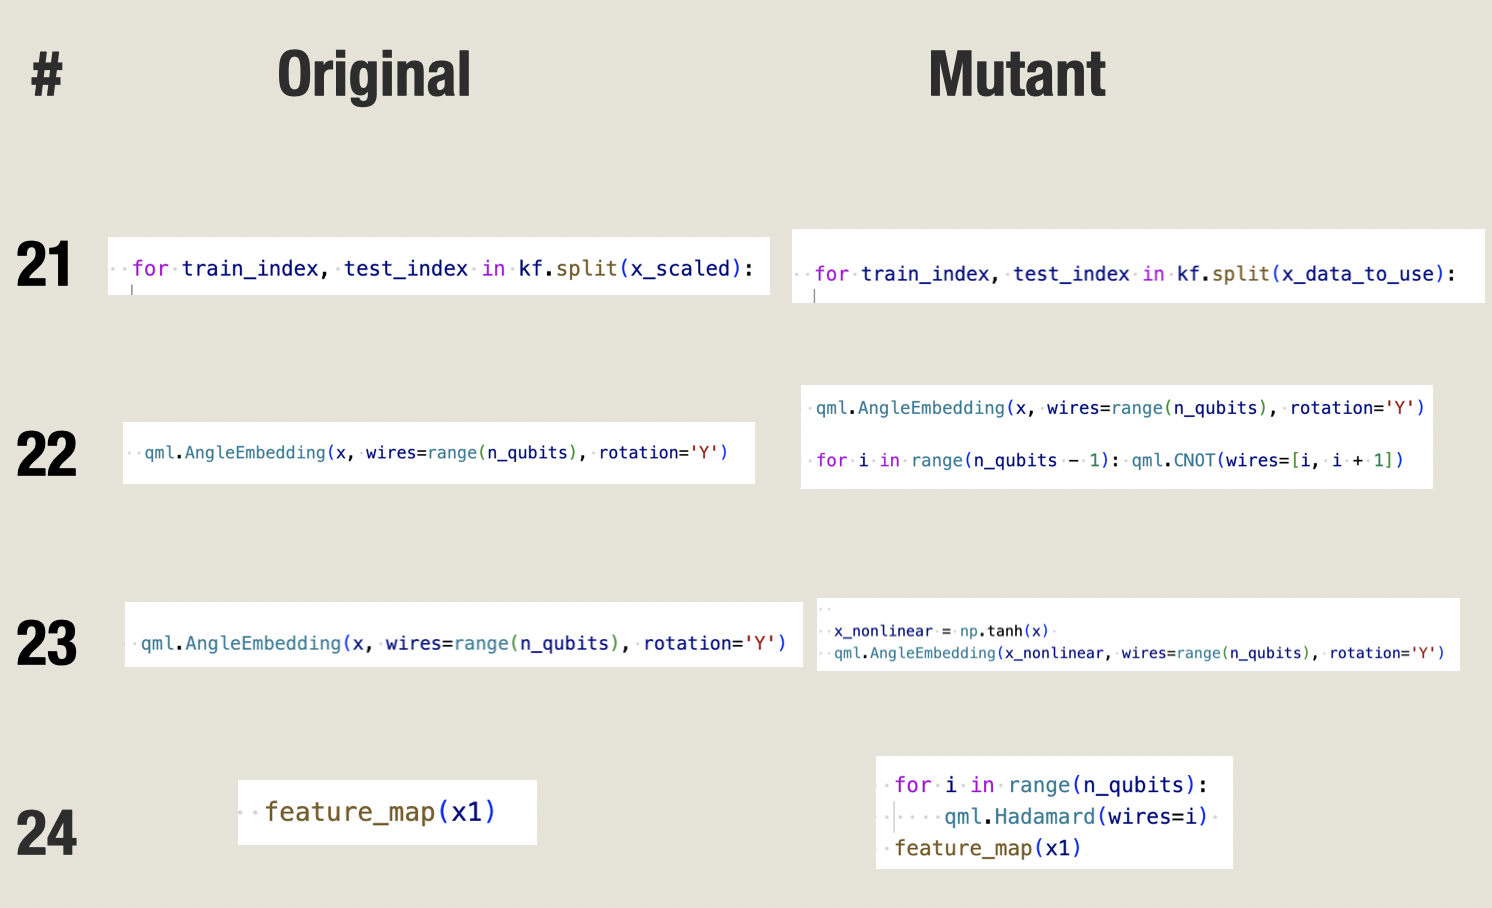
\includegraphics[height = 7 cm ,width=\linewidth]{figures/MT_6.png}
			\caption{QSVM Mutations Table \#6}
			\label{fig:16}
		\end{figure}
		
		\begin{figure}[ht!]
			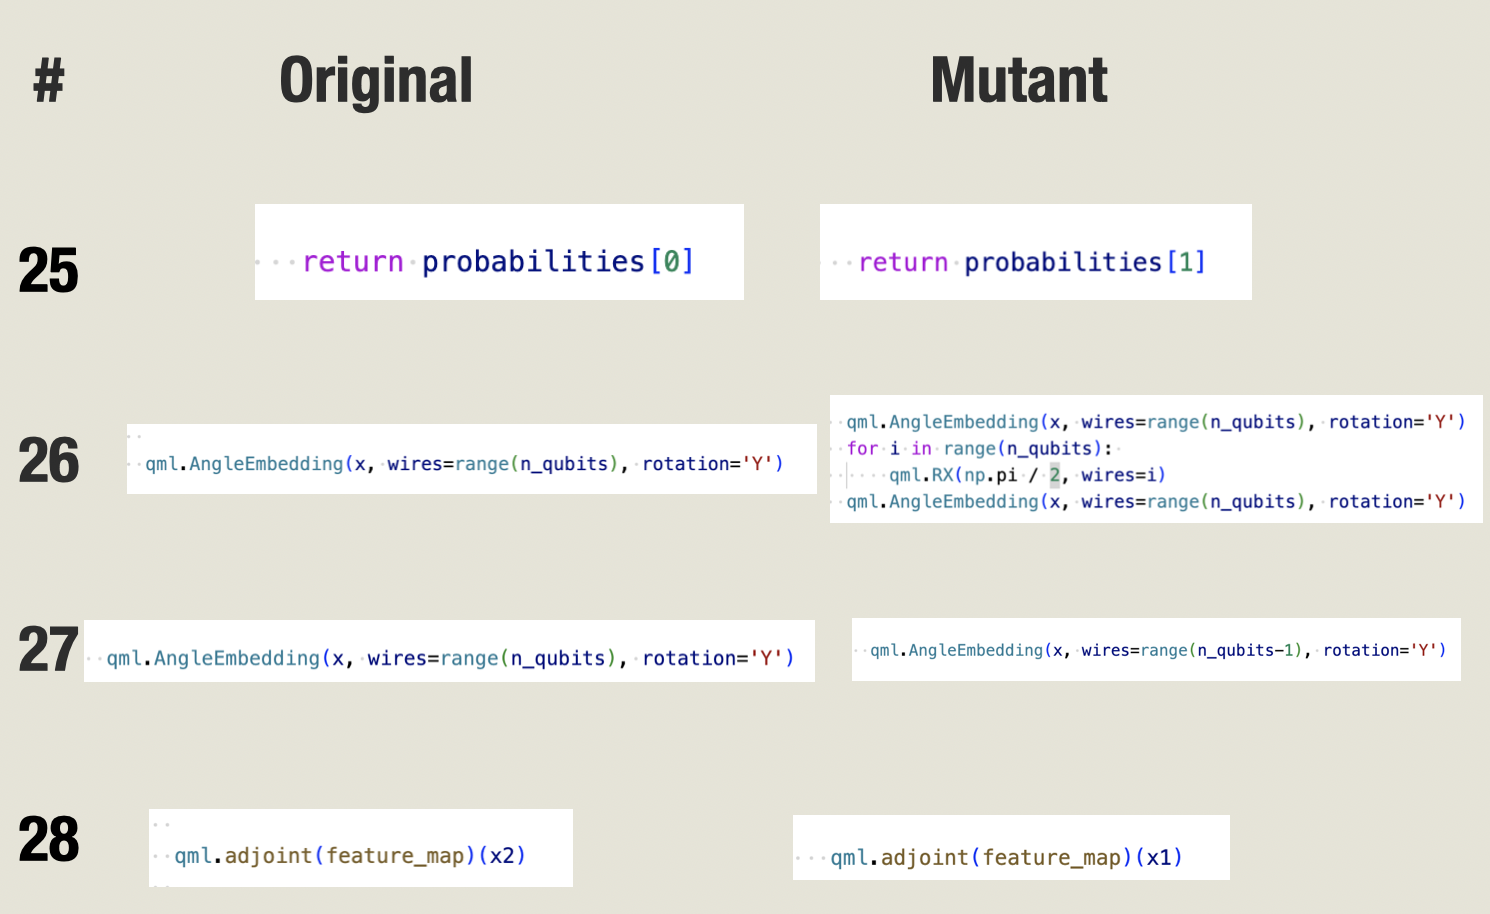
\includegraphics[height = 7 cm ,width=\linewidth]{figures/MT_7.png}
			\caption{QSVM Mutations Table \#7}
			\label{fig:17}
		\end{figure}
		
		\begin{figure}[ht!]
			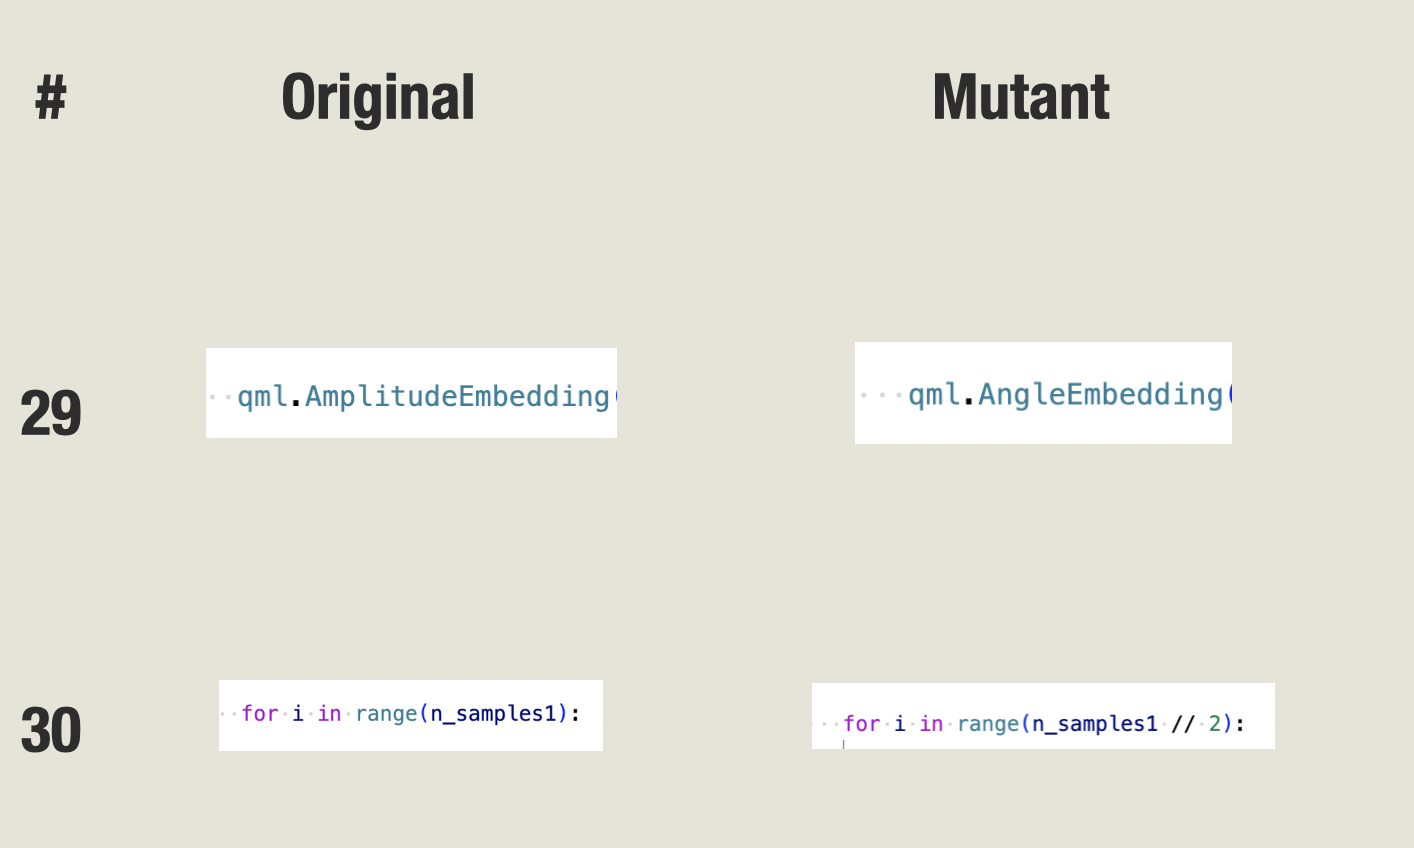
\includegraphics[height = 7 cm ,width=\linewidth]{figures/MT_8.png}
			\caption{QSVM Mutations Table \#8}
			\label{fig:18}
		\end{figure}
		
		\begin{figure}[ht!]
		\end{figure}
		
	\end{appendices}
	
\end{document}